
% PREAMBULE

%package obligatoire : type de document
\documentclass[a4paper,12pt,twoside]{book}

% encodage (pour XeLaTeX)
\usepackage{fontspec}


%si index, package pour index + makeindex avant hyperref


% le package hyperref avec des options, si en local
%\usepackage[pdfusetitle, pdfsubject ={Mémoire TNAH}, pdfkeywords={les mots-clés}]{hyperref}

%avec overleaf, utiliser :
\usepackage[xetex]{hyperref}
\hypersetup{
pdfauthor = {Justine Chainiau},
pdftitle = {VERS LA MISE EN LIGNE DES ACTES DES DUCS DE BOURBON (1356 - 1475)},
pdfsubject = {Actes princiers},
pdfkeywords = {actes princiers} {Bourbons} {édition numérique}
}

%il faut mettre au moins une langue
\usepackage[english,french]{babel}

% configurer le document selon les normes de l'école
\usepackage[margin=2.5cm]{geometry} %marges
\usepackage{setspace} % espacement qui permet ensuite de définir un interligne
\onehalfspacing % interligne de 1.5
\setlength\parindent{1cm} % indentation des paragraphes à 1 cm

\usepackage{caption}

\usepackage{longtable}

\usepackage{lettrine} % lettrines (pas obligatoire)

\usepackage{graphicx}
\usepackage{float}

\usepackage{tocbibind}

% bibliographie
\usepackage{csquotes}
\usepackage[backend=biber, sorting=nyt, style=enc,maxbibnames=10]{biblatex}
\addbibresource{bibliographie_memoire.bib}
\nocite{*}

%\usepackage{glossaries}
%\makeglossaries


% + toutes la liste des packages nécessaires à votre document (si images, tableaux, schémas, etc.)

% on pourra aussi utiliser la commande mise dans l'exemple de correction du TP1 pour enlever les titres courant qui traînent sur les pages


\author{Justine Chainiau - M2 TNAH}
\title{VERS LA MISE EN LIGNE DES ACTES DES DUCS DE BOURBON (1356 - 1475)}

% DOCUMENT
\begin{document}

 \begin{titlepage}
		\begin{center}
			
			\bigskip
			
			\begin{large}				
				ÉCOLE NATIONALE DES CHARTES\\
				UNIVERSITÉ PARIS, SCIENCES \& LETTRES
			\end{large}
			\begin{center}\rule{2cm}{0.02cm}\end{center}
			
			\bigskip
			\begin{Large}
				\textbf{Justine Chainiau}\\
			\end{Large}
		%selon le cas
			\begin{normalsize} \textit{licenciée ès lettres}\\
				\textit{diplômée de master recherche en histoire médiévale}
			\end{normalsize}
			\bigskip
			\bigskip
			
			\begin{Huge}
				\textbf{VERS LA MISE EN LIGNE DES ACTES DES DUCS DE BOURBON (1356 - 1475)}\\
			\end{Huge}
			\bigskip
			\bigskip
			\begin{LARGE}
				\textbf{Édition, encodage et chaîne de traitement au sein du projet \og Actes Princiers \fg}\\
			\end{LARGE}
			
			\begin{figure}[H]
            \centering
            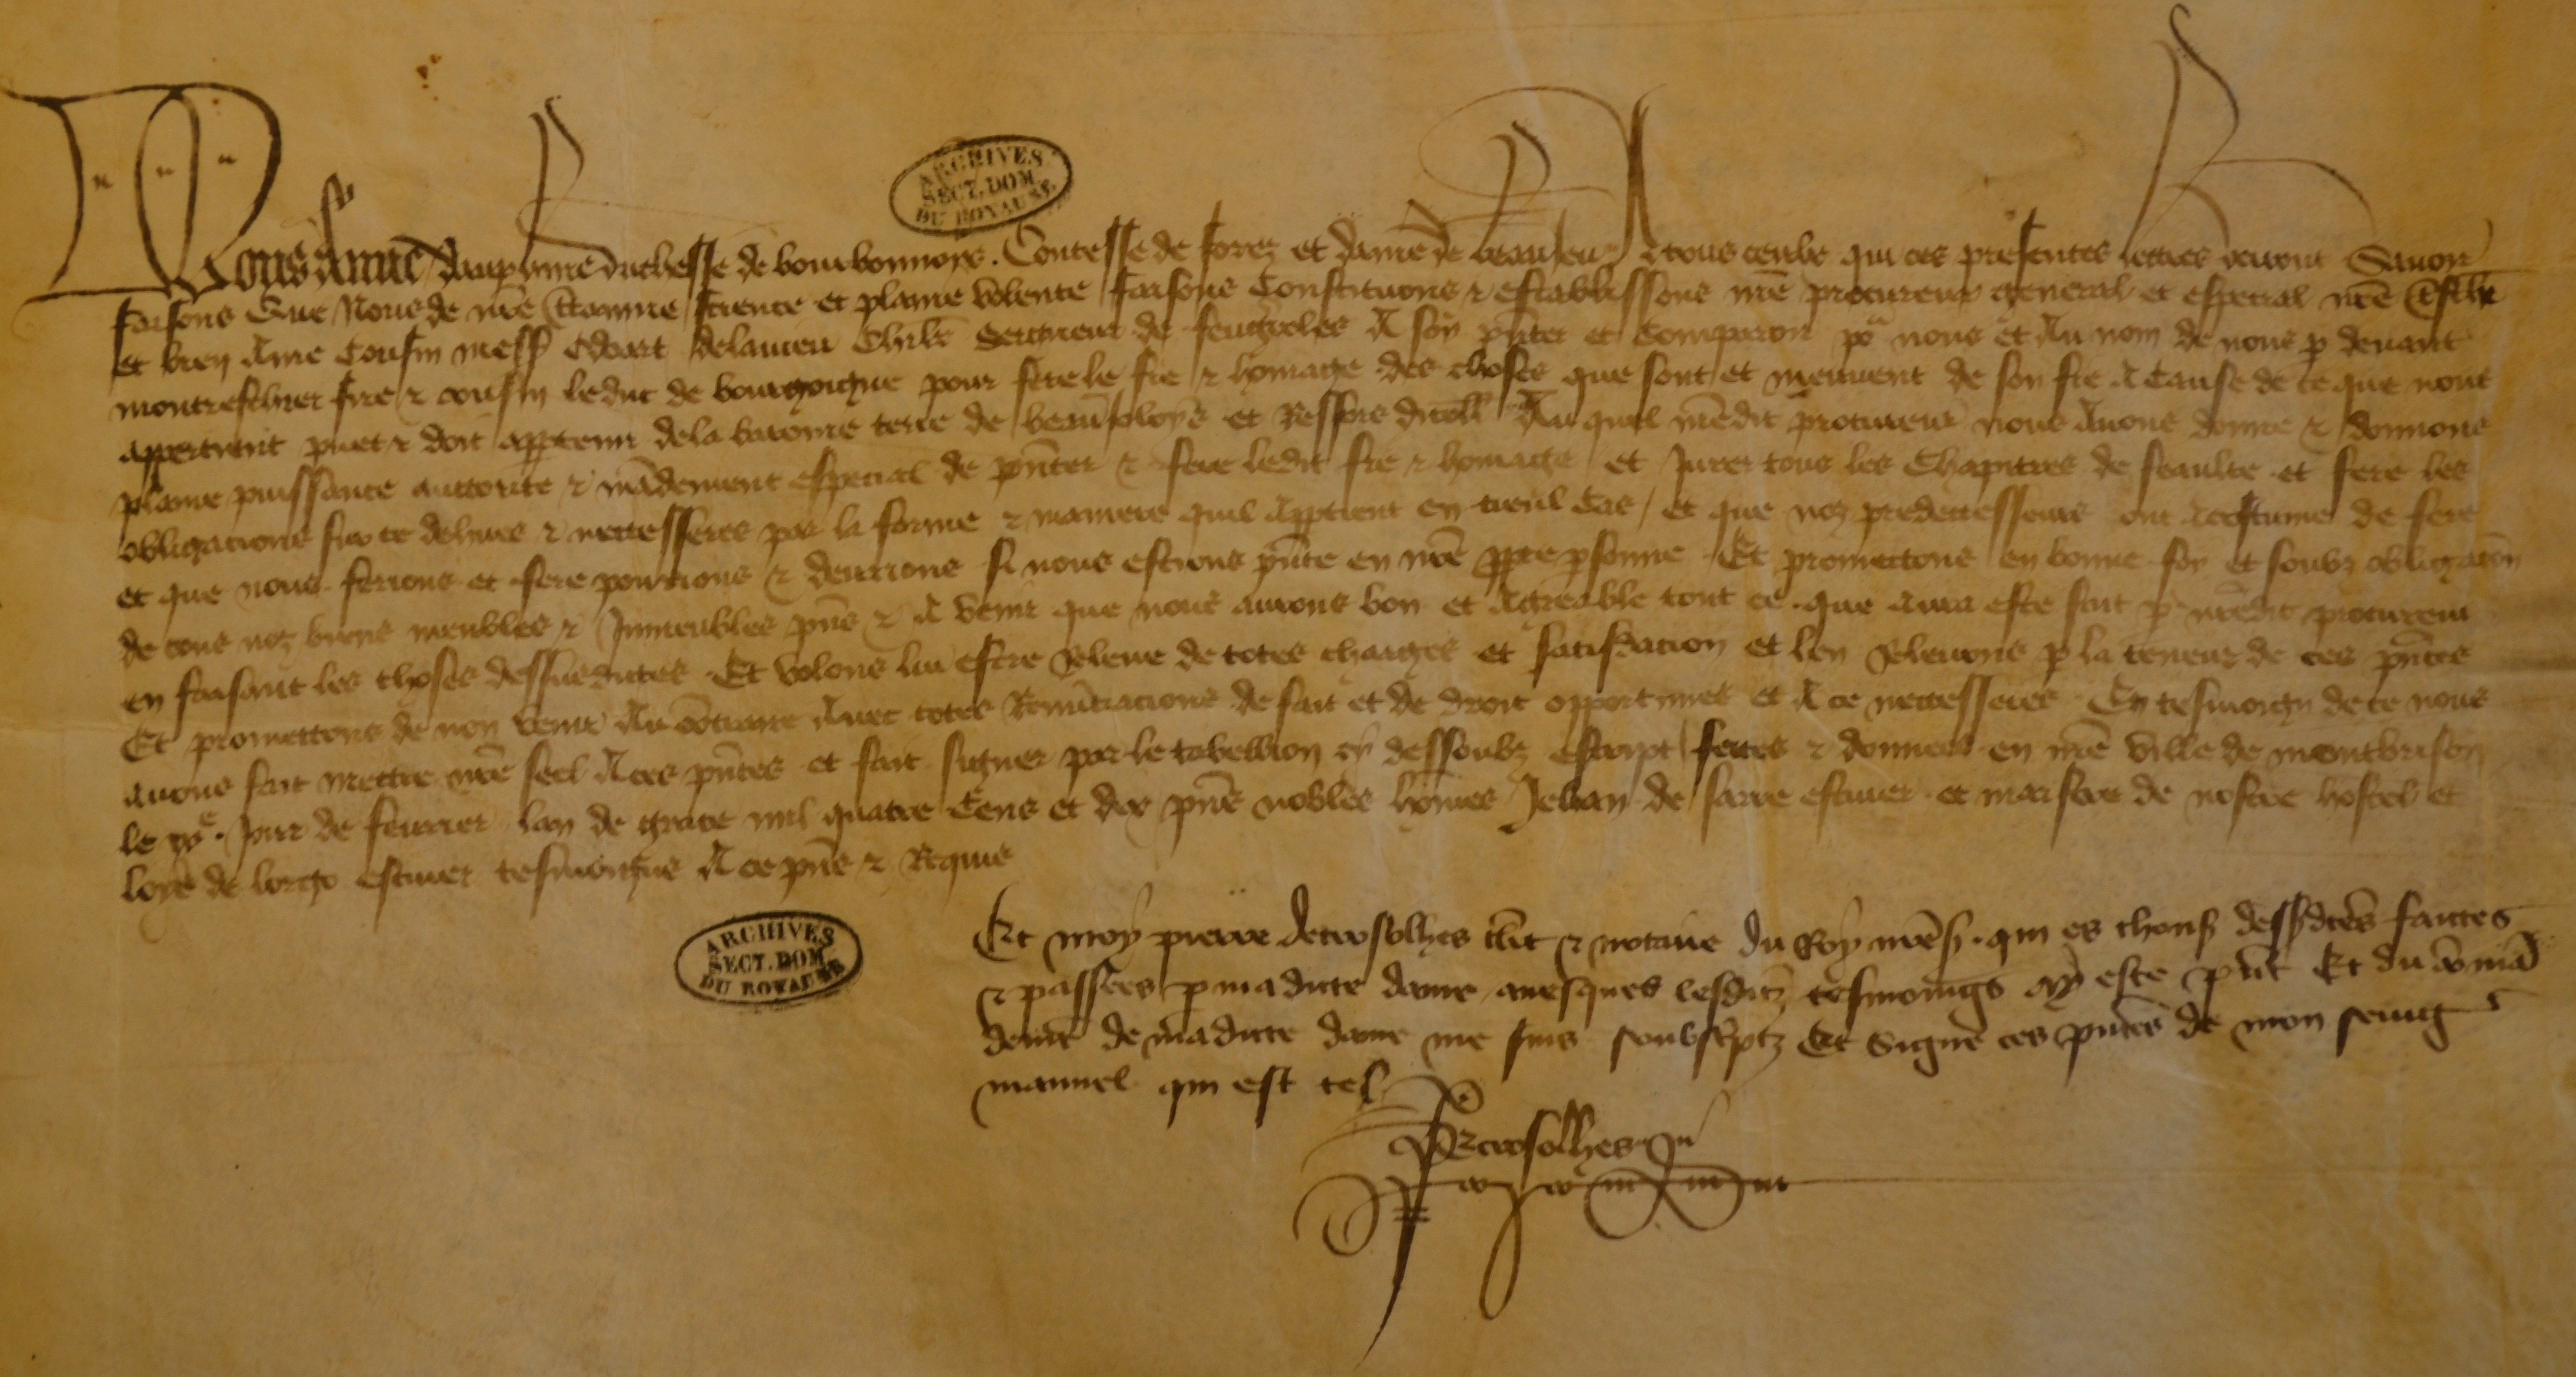
\includegraphics[scale=0.09]{img/couverture.jpg}
            \label{fig:encodage_text}
            \end{figure}
			\vfill
			
			\begin{large}
				Mémoire 
				pour le diplôme de master \\
				\og{} Technologies numériques appliquées à l'histoire \fg{} \\
				\bigskip
				2023
			\end{large}
			
		\end{center}
	\end{titlepage}
	
	\thispagestyle{empty}	
	\cleardoublepage
	
	\frontmatter
	\chapter{Résumé}
	\medskip
	Le projet \og Actes Princiers au royaume de France (\textsc{XIV}\up{e} - \textsc{XVI}\up{e} siècle) \fg \space entend procéder à l’édition numérique de plusieurs corpus d’actes inédits de princes français de la fin du Moyen Âge. Parmi ces corpus se trouvent ceux composés des actes émis par les ducs de Bourbon : Louis II, Anne Dauphine, Charles I\up{er} et Agnès de Bourgogne. 
 \newline 
    \par Ces quatre corpus ont fait l'objet d'éditions numériques via un logiciel de traitement de texte. Le présent mémoire s'attache à présenter la chaîne de traitement permettant la transformation des documents Word contenant les éditions diplomatiques des actes en des fichiers XML (TEI) en vue de leur mise en ligne. 
	\bigskip
    \bigskip
    \bigskip
    
	\textbf{Mots-clés~:} Actes princiers ; ducs de Bourbon ; chaîne de traitement ; diplomatique ; édition ; encodage ; expressions régulières ; LaTeX ; ODT ; Python ; transcription ; XML-TEI.
 \newline 
	
	\textbf{Informations bibliographiques~:} Justine Chainiau, \textit{Vers la mise en ligne des actes des ducs de Bourbon (1356 - 1475). Édition, encodage et chaîne de traitement au sein du projet \og Actes Princiers au royaume de France (\textsc{XIV}\up{e} - \textsc{XVI}\up{e} siècle) \fg}, mémoire de master \og{}Technologies numériques appliquées à l'histoire\fg{}, dir. Jean-Damien Généro et Lucence Ing, École nationale des chartes, 2023.
\newline 

    \textbf{Soutenance :} mémoire présenté et soutenu publiquement le 25 septembre 2023 à l’École nationale des chartes, devant un jury composé d’Olivier Canteaut, président, archiviste paléographe et maître de conférences, Jean-Damien Généro, ingénieur d'études du CNRS et Lucence Ing, doctorante et attachée temporaire d'enseignement et de recherche (ATER).  
    \newline 

    \textbf{Illustration de couverture :} Lettres patentes d'Anne Dauphine, AN, P 1389\up{3}, c.~314 (9 février 1410). 
	
		\newpage{\pagestyle{empty}\cleardoublepage}
	
	\chapter{Remerciements}
	
	\lettrine{M}es remerciements vont tout d'abord à mon encadrant de stage Jean-Damien Généro pour son accompagnement. Son écoute, sa disponibilité et ses conseils ont été essentiels et précieux dans la conduite des missions du stage et pour la rédaction du mémoire. 
    \newline 
    \par Je tiens aussi à remercier particulièrement Lucence Ing, pour ses relectures et ses recommandations concernant la rédaction du présent travail de recherche, et Olivier Canteaut, pour l'intérêt porté à mon travail et les informations transmises quant à ma poursuite d'étude.
    \newline 
    \par Je remercie également l'équipe pédagogique du master TNAH pour ces deux années de formation riches d'enseignements, d'acquisition de compétences et de méthodes. 
    \newline 
    \par Enfin, je remercie mes proches de m'avoir épaulée et soutenue pendant la rédaction. 

    \newpage{\pagestyle{empty}\cleardoublepage}
	
	\chapter{Liste des sigles et abréviations}

    \section*{Institutions}

    \noindent AD : Archives départementales
    \newline 
    AM : Archives municipales
    \newline 
    AN : Archives nationales
    \newline 
    BM : Bibliothèque municipale
    \newline 
    BnF : Bibliothèque nationale de France
    \newline 
    CNRS : Centre National de Recherche Scientifique
    \newline 
    CRH : Centre de recherches historiques (CNRS - EHESS)
    \newline 
    EHESS : École des Hautes Études en Sciences Sociales
    \newline 
    ENC : École Nationale des Chartes
    \newline 
    Labex : Laboratoire d'excellence
    \newline
    LAMOP : Laboratoire de médiévistique occidentale de Paris (CNRS - Paris 1)
    \newline
    UMR : Unité mixte de recherche

    \section*{Informatique et technologies numériques}

    \noindent CSV : \textit{Comma-Separated Values}
    \newline 
    HTML : \textit{Hypertext Markup Language}
    \newline 
    ODF : \textit{Open Document Format}
    \newline
    ODT : \textit{Open Document Text}
    \newline 
    PDF : \textit{Portable Document Format}
    \newline 
    TEI : \textit{Text Encoding Initiative}
    \newline 
    XML : \textit{eXtensible Markup Language}
    \newline 
    XSL : \textit{eXtensible Stylesheet Language}

    \newpage{\pagestyle{empty}\cleardoublepage}

    \chapter*{Bibliographie}\printbibliography[title=Diplomatique,heading=subbibliography,keyword=dip]\printbibliography[title=Historiographie,heading=subbibliography,keyword=histo]
    \printbibliography[title=Les ducs de Bourbon,heading=subbibliography,keyword=bourbon] 
    \printbibliography[title=Technologies numériques,heading=subbibliography,keyword=num]
    
    \addcontentsline{toc}{chapter}{Bibliographie}
 
	\chapter{Introduction} 

\par Les études sur les actes, les documents émanant d'une autorité et agissant en vertu de cette autorité\footnote{\cite{guyotjeanninDiplomatiqueMedievale2006}.}, ont dans un premier temps priorisé les actes pontificaux et royaux, \og laissant leurs homologues princiers au rang d'actes privés \fg  \footnote{Canteaut, Olivier, Moufflet, Jean-François, \og Les éditions d'actes princiers (\textsc{XII}\up{e} - \textsc{XV}\up{e} siècle) : bilan à l'ère du numérique \fg, in : \cite{guyotjeanninJeanBerryEcrit2019}.}. Les actes princiers désignent les actes émis par les princes. Le terme prince se doit d'être désambiguïsé dans ce travail. Bien que se rapportant d'ordinaire à l'héritier présomptif du trône royal au sens contemporain du terme, il ne doit ici pas être entendu pour nommer celui qui est premier par le sang ou par le rang, mais bien celui qui appartient à une maison souveraine et ne règne pas\footnote{Définition CNRTL :  \url{https://www.cnrtl.fr/definition/prince}.}. Les premiers projets consacrés aux actes princiers voient le jour au \textsc{XIX}\up{e} siècle, en Allemagne, offrant ainsi une analyse des pratiques entre princes, empereurs et évêques du Saint-Empire\footnote{\cite{bohmerRegestaImperiiInde1839}., \cite{hueberRegestenKaiserreichsUnter1877}.}. À l'instar de leurs voisins, les diplomatistes français se concentrent d'abord sur l'imitation des formes et des formules royales et c'est par ce biais que l'on voit émerger les prémices d'une diplomatique princière. Les premières recherches sont impulsées par le lancement, en 1894, par l'Académie des inscriptions et belles-lettres, d'une nouvelle série, en plus de celles dédiées aux actes royaux et pontificaux, consacrée aux actes des \og grands feudataires \fg\footnote{\cite{guyotjeanninJeanBerryEcrit2019}.}. Cette série s'ouvre avec la publication des actes d'Henri II Plantagenêt (1151-1189) relatifs à la France\footnote{\cite{delisleRecueilActesHenri1909}.}. Malheureusement, cette entreprise n'est pas poursuivie et il faut attendre la fin du XX\up{e} siècle pour assister au départ de nouveaux projets. La plupart de ces derniers se focalisent sur le début du bas Moyen Âge. On observe une raréfaction des éditions de documents des \textsc{XII}\up{e} - \textsc{XV}\up{e} siècle, à l'exception des cas bourguignon, breton et gascon\footnote{Annexe Répartition chronologique des éditions et catalogues d'actes princiers produits (espace français actuel), in Canteaut, Olivier, Moufflet, Jean-François, \og Les éditions d’actes princiers (\textsc{XII}\up{e} - \textsc{XV}\up{e} siècles) : bilan à l’ère du numérique \fg , in : \cite{guyotjeanninJeanBerryEcrit2019}.}. 

\par Force est de constater, en plus des disparités chronologiques, des disparités géographiques. Concernant les actes des ducs de Bretagne, nous pouvons citer les travaux de Michael Jones, pour les actes de Charles de Blois~(1341~-~1364), Jeanne de Penthièvre~(1341~-~1365, † 1384) et Jean \textsc{IV}~(1365~-~1399), de Marjolaine Lémeillat pour les actes de Pierre de Dreux~(1213~-~1221) et de Jean I\up{er}~(1221~-~1286), ainsi que ceux de Jean Kerhervé sur la chancellerie de Bretagne au temps du duc François \textsc{II}~(1458~-~1488), de sa fille la duchesse Anne~(1488~-~1514) et du premier mari de celle-ci, le roi de France Louis \textsc{XII}~(1498~-~1515) \footnote{\cite{jonesRecueilActesCharles2016}. \newline \cite{jonesRecueilActesJean1980}. \newline \cite{lemeillatActesPierreDreux2013}. \newline \cite{kerherveChancellerieBretagneSous2001}.}. Le duché de Bourgogne est également l'objet de travaux, parmi lesquels ceux d'Anne-Lise Courtel sur la Bourgogne pour les ducs capétiens, puis, d'Henri Stein pour les ducs Valois, Philippe le Hardi~(1363~-~1404), Jean sans Peur~(1404~-~1419) et Philippe le Bon~(1419~-~1467) et de Sonja Dünnebeil pour les actes de Charles le Téméraire~(1467~-~1477)\footnote{\cite{courtelChancellerieActesEudes1977} \newline \cite{steinCatalogueActesCharles1999}.}. Pierre Cockshaw a également étudié le personnel de la chancellerie de Bourgogne-Flandre\footnote{\cite{cockshawPersonnelChancellerieBourgogneFlandre1982}.}. Même si elles sont majoritaires, les entreprises d'édition ne concernent pas que les deux maisons précédemment citées. John Benton et Michel Bur ont étudié les actes du comte de Champagne, Henri le Libéral~(1152~-~1181)\footnote{\cite{bentonRecueilActesHenri2009}.}. La chancellerie dauphinoise sous Humbert~II~(1333~-~1349) a aussi engendré le dépouillement d'actes par Chantal Reydelet \footnote{\cite{reydeletChancellerieHumbertII1974}.}. Ces disparités géographiques et chronologiques s'expliquent par le fait que pour la période étudiée, les corpus sont importants et très dispersés. Nombre des travaux sur les actes princiers se sont limités à des analyses, à des catalogues, plutôt qu'à une édition complète face à l'abondance de la documentation. 
\newpage 

\par Toutefois, comme l'indique Olivier Canteaut, \og le développement de l'édition électronique scientifique et, plus globalement, les perspectives offertes par les humanités numériques stimulent en effet depuis plus d'une décennie la réalisation d'amples corpus d'actes et la diplomatique princière laïque bénéficie de ce regain d'intérêt \fg \footnote{Canteaut, Olivier, Moufflet, Jean-François, \og Les éditions d’actes princiers (\textsc{XII}\up{e} - \textsc{XV}\up{e} siècle) : bilan à l’ère du numérique \fg, in :\cite{guyotjeanninJeanBerryEcrit2019}.}. En effet, l'édition numérique offre l'opportunité d'entamer de vastes chantiers d'identification et de regroupement de sources et d'en publier un premier état. Cette opportunité n'est pas négligeable dans le cas où les données sont éclatées sur le territoire, dans différents services d’archives et nécessitent le travail conjoint de plusieurs chercheurs. Ce regain s'applique dans un premier temps à publier les analyses des actes\footnote{Les actes pontificaux en France, \url{https://qed.perspectivia.net/gallia-pontificia-online/}. \newline Regesta Imperii Online, \url{http://opac.regesta-imperii.de/lang_en/}.}, à d'autres supports comme les cartulaires et les chartriers \footnote{Digitale Monumenta Germaniae Historica \url{https://www.dmgh.de/}. \newline Cartulaires d'Île-de-France \url{http://elec.enc.sorbonne.fr/cartulaires/}. \newline Base des actes normands médiévaux Scripta \url{https://www.unicaen.fr/scripta/}. \newline Corpus de la Bourgogne au Moyen Âge CMBA \url{http://www.cbma-project.eu/}.}, mais aussi aux travaux déjà imprimés. Le projet \og Corpus des actes royaux de la France médiévale \fg \space (CARo) s'attache à rendre accessible sous forme numérique les actes des rois de France, de Charles le Chauve~(875~-~877) à Philippe Auguste~(1180~-~1223), édités par l’Institut de France\footnote{Corpus des actes royaux, en ligne : \url{https://lamop.hypotheses.org/category/corpus-des-actes-royaux-caro}.}. Ces entreprises sont motrices et participent au développement d'éditions dédiées aux actes des grands. C'est dans ce contexte que s'inscrit le projet consacré aux actes princiers. 
\newline 

\par Le projet \og Actes princiers au royaume de France (\textsc{XIV}\up{e} - \textsc{XVI}\up{e} siècle) \fg \space est porté par le professeur des universités Olivier Mattéoni et rassemble quatre institutions : deux unités mixtes de recherche (UMR) que sont le Laboratoire de Médiévistique occidentale de Paris (LaMOP, Paris 1 - CNRS\footnote{Laboratoire de médiévistique occidentale de Paris, \url{https://lamop.pantheonsorbonne.fr/}.}), qui porte le projet et le Centre de recherches historiques (CRH, CNRS - EHESS), le centre de recherche de l'École Nationale des Chartes, Centre Jean Mabillon, et le département du Moyen Âge et de l’Ancien régime des Archives nationales. L'ambition du projet est de procéder à l’édition numérique de plusieurs corpus d’actes inédits issus des chancelleries des princes de sang de la fin du Moyen Âge. Ces corpus comprennent les actes des ducs et duchesses de Bourbon et du duc Jean de Berry~(1360~-~1416). Leur nombre est voué à s'accroître et à comporter par la suite d'autres actes princiers comme ceux de la maison d'Orléans et de la maison d'Anjou. Le projet comprend le développement d’un site web et l’encodage d’une première série d’actes : ceux de Louis \textsc{II}~(1356~-~1410) et de Charles I\up{er}~(1434~-~1456) de Bourbon et de leurs épouses Anne Dauphine~(1371~-~1410, † 1417) et Agnès de Bourgogne~(1434~-~1456, † 1476)\footnote{Annexe Généalogie de la famille ducale de Bourbon.}. 
\newpage 

\par Louis II de Bourbon devient duc en 1356, dans des conditions difficiles. À la suite de la défaite de Poitiers, il est envoyé comme otage en Angleterre en échange de la libération du roi de France Jean II~(1350~-~1364)\footnote{\og Poitiers\fg, in : \cite{favierGuerreCentAns1980}, p.181.}. Ses années de captivité entravent considérablement la gouvernance du duché. À son retour, en 1366, il soude la noblesse autour de l’ordre de chevalerie de l’écu d’or et mène une politique d'expansion territoriale par le biais d’alliances. Son mariage avec Anne de Forez, héritière du comté de Forez, en 1371, sanctionne le rattachement du comté à la principauté bourbonnaise. En 1400, le mariage de son fils Jean de Bourbon~(1410~-~1434) avec Marie de Berry~(1416~-~1434) prévoit l’intégration du duché d’Auvergne à la mort du duc Jean de Berry, intégration qui sera effective en 1425. L’Auvergne est un apanage qui doit revenir au domaine royal dans le cas où le duc, père de Marie de Berry, n’a pas d’héritier mâle. Toutefois, Jean de Berry et Louis II de Bourbon obtiennent du conseil royal et de Charles VI~(1380~-~1422) que cet apanage revienne aux Bourbons du fait du mariage de leurs enfants. Cette expansion participe au développement institutionnel notable du duché impulsé par le duc, qui se traduit par d’importantes réformes avec la création d’un office de trésorier général (1372) et d'une chambre des comptes (1374)\footnote{\og Les ducs de Bourbon, le roi et le royaume de France à la fin du Moyen Âge \fg, in : \cite{matteoniBourbonsLeurBibliotheque2022}.}. Olivier Mattéoni parle d'une \og fièvre normative \fg \space pour les domaines des finances et de la justice\footnote{\cite{matteoniProposOrdonnanceFinance2019}.}. L'agrandissement de la principauté et les réformes qui en découlent génèrent une importante production documentaire d'actes écrits servant à créer ou confirmer des actions juridiques\footnote{\cite{guyotjeanninDiplomatiqueMedievale2006}.}. La production de ces actes s’inscrit dans un projet de réforme du gouvernement rendu nécessaire par l'agrandissement de la principauté. Les années 1370 sont marquées par une réorganisation de la chancellerie avec l’augmentation du nombre de secrétaires et une rationalisation des règles de confection des actes avec notamment la généralisation et l’obligation de la signature\footnote{\cite{matteoniEcriturePouvoirPrincier2011}.}. 
\newline 

\par En 1410, Jean I\textsuperscript{er} succède à son père à la tête d’une principauté bien administrée. Il est duc de 1410 à 1434, mais exerce peu la réalité du pouvoir, car il est fait prisonnier par les Anglais en 1415 à Azincourt\footnote{\og Les ducs de Bourbon, le roi et le royaume de France à la fin du Moyen Âge \fg, in : \cite{matteoniBourbonsLeurBibliotheque2022}.}. La production documentaire du duc Jean I\up{er} et de son épouse Marie de Berry est exclue de cette étude. Le travail de recensement des actes s'est concentré sur ceux de Louis II et Charles I\up{er} et de leurs épouses du fait de leurs réformes dans l'administration bourbonnaise et des acquisitions territoriales importantes sous leurs règnes. De plus, les actes dénombrés pour le couple Jean I\up{er} et Marie de Berry sont très peu nombreux : seuls cinquante-neuf actes ont pu être recensés (et quarante-quatre d'entre eux sont établis avant 1415)\footnote{\cite{generoChancellerieCharlesIer2018}.}. Pendant la captivité du duc, les femmes administrent le duché : d’abord Anne Dauphine, comme duchesse douairière jusqu’en 1417, puis Marie de Berry. La période est caractérisée par la réconciliation avec la maison de Bourgogne qui se concrétise par l'alliance matrimoniale entre Charles de Bourbon et Agnès de Bourgogne, la fille du duc de Bourgogne Jean Sans Peur, en 1425. 
\newline 

\par Charles I\up{er} devient duc en 1434, mais en raison de la captivité de son père, il assure le gouvernement du duché avant. Il bénéficie d'une proximité importante avec le roi de France Charles VII~(1422~-~1461) qui le nomme lieutenant en Languedoc et dans les marches est du royaume et dont il est le conseiller dès les années 1420\footnote{\cite{leguaiSeigneurieEtatBourbonnais1975a}.}. Il est également choisi par ce dernier pour diriger la délégation royale à la paix d’Arras, en 1435. Son mariage avec Agnès de Bourgogne le met en possession du duché d'Auvergne, ce qui contribue à affermir son influence. Il noue des alliances avec les autres princes du royaume et entre en rébellion contre le roi lors de la Praguerie en 1440\footnote{En 1440, révolte des grands contre Charles VII (à laquelle se joignit le Dauphin).}. Après l'échec de cette dernière, il se concentre sur l'administration et les finances avec la création de l'office de contrôleur général. Son principat est caractérisé par le renforcement des cadres institutionnels de la principauté (finances, fiscalité… )\footnote{\og Les ducs de Bourbon, le roi et le royaume de France à la fin du Moyen Âge\fg, in : \cite{matteoniBourbonsLeurBibliotheque2022}.}. Il cherche également à s'assurer le soutien de la noblesse, comme le montre la création de l'Armorial de Bourbonnais et de Forez\footnote{Armorial : Registre ou catalogue contenant les armes ou armoiries de la noblesse d'un royaume, d'une province, d'une ville, d'une famille, dessinées, peintes ou décrites. Définition CNRTL. \cite{deboosArmorialAuvergne1998}.}. La cour des ducs de Bourbon, implantée à Moulin, devient alors un centre artistique accueillant sculpteurs, musiciens, écrivains\footnote{\cite{leguaiSeigneurieEtatBourbonnais1975a}.}. L'épouse de Charles I\up{er}, Agnès de Bourgogne, n'est pas sans jouer un rôle diplomatique. Elle fait régulièrement l'intermédiaire entre son mari et son frère, et s'attache à mener une politique de pacification entre les deux familles \footnote{\cite{leguaiAgnesBourgogneDuchesse1996}.}. Sept de ses onze enfants sont notamment élevés à la cour de Bourgogne. La fin du principat de Charles I\up{er} est marquée par sa maladie. Il meurt le 4 décembre 1456 et son épouse lui survit jusqu'en 1476.
\newpage 

\par L'objectif du stage dans le projet « Actes princers » est de participer à la conception d'une chaîne de traitement afin de transformer des fichiers ODT contenant les éditions diplomatiques d’actes bourbonnais en des fichiers XML (TEI), pour assurer leur mise en ligne. L'un des enjeux est de tester les différentes solutions de transformation pour les documents afin de déterminer la plus adaptée au corpus, et pour des besoins futurs. Ensuite, les métadonnées associées aux corpus sont extraites via des scripts Python afin de les incorporer dans les fichiers XML/TEI produits. Ces derniers sont intégrés à une application Flask prototypée pour leur mise en ligne. 
\newline 

\par Ce travail est accompagné d'un livrable technique situé dans un repository GitLab\footnote{Justine Chainiau, Chaîne de traitement des actes princiers, en ligne : \url{https://gitlab.huma-num.fr/medieval-acts/princely-acts/stage_actes_princiers.git}.}. Il comprend les fichiers contenant les actes édités sous différents formats (ODT, PDF, XML) ainsi que les fichiers CSV contenant les métadonnées des actes. Il comprend également une chaîne de traitement de données (scripts Python) codée par les ingénieurs du projet, fonctionnelle et documentée. Il est complété par le descriptif des étapes du travail et du code nécessaire à la réflexion sur l’édition numérique et la mise en ligne d'actes princiers. 
\newline 

\par L'enjeu de ce travail de recherche autour du projet \og Actes Princiers \fg \space est de contribuer à une meilleure connaissance de la diplomatique princière qui est encore obscure pour la fin du Moyen Âge en France. 
\par Ce projet d'édition s'articule d'abord autour de l'édition des actes dispersés des princes de Bourbon, Louis II, Anne Dauphine, Charles I\up{er} et Agnès de Bourgogne. 
\par Il s'accompagne ensuite d'une importante réflexion sur la transformation des éditions, du traitement de texte vers l'encodage, afin de choisir les opérations de préparation, le langage d'encodage et le convertisseur les plus adaptés. 
\par Enfin, l'aboutissement du projet réside dans la conception d'une chaîne de traitement des actes via la technologie Python, afin de les pourvoir d'une structuration optimale nécessaire à la mise en ligne des données. 

\newpage
\thispagestyle{empty}
\mbox{}
\newpage
	
	\thispagestyle{empty}
	\cleardoublepage
	
	\mainmatter
	
	% là, le corps du mémoire, généralement TROIS parties
	
	% possibilité d'avoir un document main.tex peu rempli, et chaque partie appelée par \input{} par exemple
    \part{L'édition numérique des corpus de Louis II, d'Anne Dauphine et de Charles I\up{er} et d'Agnès de Bourgogne}


\newpage

	\chapter{Présentation du corpus}

\vspace*{\stretch{1.3}} 
\par Le corpus dénombre huit cent vingt-trois actes, avec presque autant d'actes pour chaque couple de prince. Quatre cent douze actes sont recensés pour Louis II (333) et Anne Dauphine (79) et quatre cent six actes pour Charles I\textsuperscript{er} (379) et Agnès de Bourgogne (32). L'étude de ce corpus est permise par la conservation des différents actes étudiés. Lorsqu'on y regarde de plus près, on est vite confronté  à la dispersion de la documentation. Aucune série documentaire ne se rapporte à la chancellerie ni ne contient l'enregistrement des actes des ducs de Bourbon par cette dernière\footnote{\cite{matteoniEcriturePouvoirPrincier2011}.}.
\vspace*{\stretch{0.7}} 
\newpage 

\section{Dispersion des actes}
\label{I.1.1}

\par Les actes des Bourbons sont conservés depuis le \textsc{XII}\up{e} siècle\footnote{\cite{huillard-brehollesTitresMaisonDucale1867}.}. Sous la première maison de Bourbon, les seigneurs de Bourbon-Dampierre, les pièces originales sont déposées dans des coffres ou des layettes et les lettres sont petit à petit transcrites dans des cartulaires. L'accroissement de la production documentaire donne lieu à la réalisation d'inventaires dès le \textsc{XIV}\up{e} siècle. Après la création de la chambre des comptes de Moulins, en 1374, le duc Louis II  ordonne que tous les actes, terriers, lettres et écritures touchant au domaine (nominations, lettres de dons et de grâce, ordonnances) y soient remis\footnote{\cite{huillard-brehollesTitresMaisonDucale1867}.}. La chambre des comptes se sédentarise à Moulins et fonctionne avec une régularité croissante. Le \og Trésor des chartes\fg \space du Bourbonnais s'agrandit et est complété par les inventaires des actes conservés dans les territoires nouvellement acquis. En effet, Louis II maintient les Chambres des comptes du comté de Forez à Montbrison et de la seigneurie de Beaujolais à Villefranche. En 1527, cinq ans après de la fuite du dernier duc de Bourbon, le connétable Charles III~(1505~-~1523), François I\up{er}~(1515~-~1547) confisque tous les biens féodaux des Bourbons tenus en apanage\footnote{\cite{huillard-brehollesTitresMaisonDucale1867}.}. L'administration des domaines revient alors à la mère du roi, Louise de Savoie~(1476~-~1531), petite fille du duc de Bourbon Charles I\up{er}, qui en revendique alors la possession. À sa mort, cet héritage contesté retourne à la couronne. Les chambres des comptes du duché de Bourbon sont supprimées, leur juridiction est transférée à la chambre des comptes de Paris et le Trésor des chartes du Bourbonnais y est rapatrié après la réalisation d'un inventaire par Jacques Luillier\footnote{\cite{huillard-brehollesTitresMaisonDucale1867}.}. Au début du \textsc{XVIII}\up{e} siècle, pour éviter les pertes, les liasses sont reliées et converties en volumes et les sceaux sont coupés. Le tout est réuni dans le dépôt de la chambre d'Anjou. La série de titres et de registre qui était restée à Moulins est détruite sous le Directoire comme entaché de féodalité, celle de Villefranche subit de nombreuses pertes et les archives du Forez à Montbrison sont transférées à Lyon au bureau des trésoriers de France. L'inventaire des \textit{Titres des Bourbons}\footnote{\cite{huillard-brehollesTitresMaisonDucale1867}.}, édité par les archivistes Alphonse Huillard-Bréholles et Albert Lecoy de la Marche au \textsc{XIX}\up{e} siècle, dresse, de manière chronologique, la liste des actes des trois chambres des comptes du duché qui sont conservés dans la série P des Archives nationales, dans les fonds des anciennes Chambre des comptes du duché de Bourbon (P 1355 à P 1402)\footnote{Archives nationales, Série P, Chambre des comptes et comptabilité, en ligne : \url{http://www.archivesnationales.culture.gouv.fr/chan/chan/fonds/EGF/SA/SAPDF/Egfn-p.pdf}.}. La majorité des actes du corpus (318) provient de cette série P, mais quelques actes ont également été identifiés dans les séries J~(43) et K~(7)\footnote{Série J, Trésor des Chartes - Série K, Monuments historiques.}. 

\par Une autre partie importante du corpus est issue des services d'archives départementales (221). La localisation de ces institutions de conservation révèle la géographie du duché de Bourbon. La majorité des actes identifiés aux Archives départementales provient du service de la Loire (150). Le territoire de ce département correspond à celui de l’ancien comté de Forez, qui est rattaché à la principauté par héritage lors du mariage, en 1371, entre Louis II et Anne Dauphine. D'autres actes sont conservés dans les services de l'Allier, sur le territoire du duché de Bourbonnais, du Puy-de-Dôme, sur le territoire du duché d'Auvergne et du Cantal, dont une partie était autrefois rattaché au duché d'Auvergne. Les actes conservés dans les services d'archives municipales nous éclairent également sur la géographie de la production documentaire des ducs de Bourbon. Des actes ont été identifiés dans les services d'archives de Moulins, capitale du duché. Louis II y fait construire un château en 1375 et s'y installe définitivement. Ses successeurs font de même et la ville devient alors le siège de la cour ducale et un centre culturel important\footnote{« Les ducs de Bourbon, le roi et le royaume de France à la fin du Moyen Âge », in : \cite{matteoniBourbonsLeurBibliotheque2022}}. D'autres actes ont été retrouvés aux Archives municipales de Riom, la capitale du duché d'Auvergne, et de Montluçon, une autre ville d'envergure. Ils sont, pour la grande majorité, relatifs à l'administration de la principauté bourbonnaise. 
\newline 

\par La localisation des institutions de conservation témoigne également des relations entretenues par les Bourbons avec les autres princes. Des actes proviennent des services d'archives départementales de la Côte-d'Or (24), et du Nord (ancien duché de Flandres) pour le corpus de Charles I\up{er}, et témoignent des alliances et accords passés avec les ducs de Bourgogne. D'abord, son mariage, en 1425, avec Agnès, la fille du duc Jean Sans Peur\footnote{AN, P 1370\up{2}, c. 1919. (4 février 1425).}, puis des traités et des abstinences de guerre conclues avec Philippe le Bon\footnote{AD Côte-d’Or, B 11918, c. 118. (4 décembre 1434).}. En moindres proportions, des actes ont été recensés dans les services d'archives départementales de la Loire-Atlantique et du Tarn. Ils témoignent des liens entre les différents princes et des différentes alliances et trêves conclues pendant la guerre de Cent Ans\footnote{AD Nord, B 304, c. 15.660 (7 septembre 1435) — AD Loire-Atlantique, E 121-1, c. 42 (4 avril 1441).}. Le reste des actes du corpus provient de la Bibliothèque nationale de France (172), notamment de la collection Gaignière\footnote{BnF, ms. fr. 22388 et 22390.}, ou de collections d'érudits des \textsc{XVII}\up{e} - \textsc{XVIII}\up{e} siècles (La Mure, Hozier, Tripperet). 

\par Le corpus étudié est donc dispersé géographiquement, institutionnellement et chronologiquement dans la mesure où il se déploie sur plus d'un siècle. 

\section{Répartition chronologique des actes}
\label{I.1.2}

\par Le corpus étudié couvre la période allant de 1357 à 1475. Nous pouvons établir une première période allant de 1357 à 1410 pour Louis II et jusqu'à 1417 pour Anne Dauphine. Puis, une seconde période de 1421 à 1456 pour Charles I\textsuperscript{er} et jusqu'à 1475 pour Agnès de Bourgogne. Les veuves des deux ducs leur survivent et continuent à produire des actes en raison des circonstances politiques. Anne Dauphine continue à émettre des actes pour le comté de Forez, dont elle est l'héritière, et au début de la captivité de Jean I\up{er}.
\newline 

\par À partir du graphique ci-après, nous pouvons établir une moyenne d'environ dix actes par an pour notre corpus. Le nombre d'actes est en deçà au début du principat de Louis II. En revanche, on observe une augmentation des écrits à partir des années 1380, qui fait suite à ses réformes administratives. Ensuite, le nombre d'actes recensés est plutôt stable jusqu'à sa mort. 

\begin{figure}[ht]
\centering
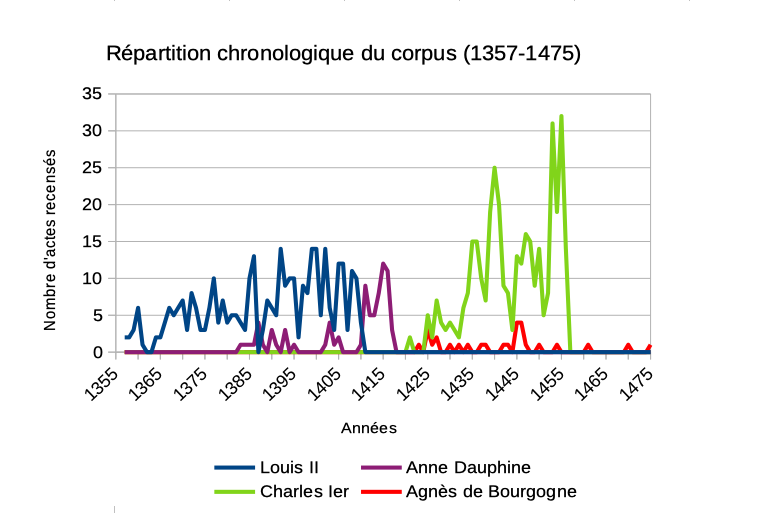
\includegraphics[scale=0.6]{img/repartition_chronologique_corpus.png}\caption{Répartition chronologique des actes du corpus.} \label{fig:chrono_actes}
\end{figure}
\newpage 

\par La diminution du nombre d'actes entre le principat de Louis II et celui de Charles~I\textsuperscript{er} s'explique par le fait que Charles I\up{er} n'est pas le successeur direct de Louis II d'une part. D'autre part, les actes du duc Jean~I\textsuperscript{er} et de son épouse Marie de Berry ne sont pour l'instant pas traités par le projet Actes princiers. Néanmoins, des actes sont quand même le fait de la duchesse Anne Dauphine, pour laquelle on observe une nette augmentation à la mort de son époux, et de Charles de Bourbon, qui commence à administrer le duché pendant la captivité de son père. Le nombre d'actes recensés pendant le principat de Charles I\textsuperscript{er}, à partir de 1434, est caractérisé par une augmentation par rapport à la période de Louis II, ce qui peut faire penser à une émission de plus d'actes sur une plus courte période. Cette augmentation peut s'expliquer par la consolidation d'une administration déjà stable, mais surtout par le biais documentaire qu'induit le corpus. Nous ne pouvons en effet pas chiffrer la part de la production totale de la chancellerie bourbonnaise qui nous est parvenue par rapport à celle qui a été perdue. L'un des pics de production peut être documenté plus assurément. Il s'agit de l'augmentation au début des années 1440, pendant la Praguerie\footnote{\cite{generoChanceliersSecretairesChancellerie2021}.}, avec de nombreuses nominations de capitaines-châtelain et de capitaines de guerre\footnote{BnF, ms. fr. 22299, folio 9 (20 juillet 1440) — BnF, ms. fr. 22299, folio 9 (30 juillet 1440).}. Cependant, le second pic en 1455, peu avant la mort du duc, avec de nombreuses nominations et fondations pieuses afférentes au duché\footnote{\cite{matteoniServirPrinceOfficiers1994}.}, ne peut réellement être explicité. Il est certainement plutôt dû à un effet de source qu'à un regain administratif à la fin de la vie de Charles I\textsuperscript{er}. En effet, nous conservons un registre d'enregistrement d'actes de la Chambre des comptes du comté de Forez, à Montbrison, qui contient des copies de lettres de nomination d'officiers des années 1450 aux années 1470\footnote{AD Loire, B 1844.}.
\newline 

\par L'émission des actes est plutôt 
constante malgré quelques variations dues au contexte politique du duché pour la période étudiée. Néanmoins, il ne faut pas perdre de vue que ce graphique omet les actes qui ont été perdus, ou qui n'ont pas encore été retrouvés, et comptabilise le corpus étudié, soit les actes qui ont été identifiés. Ces derniers représentent une masse conséquente aux natures et aux typologies variées. 
\newpage 

\section{Typologie des actes}
\label{I.1.3}

\par L'étude du corpus révèle les différentes typologies documentaires. Parmi les actes à forte valeur juridique, on trouve des chartes, dont la valeur est perpétuelle, et des lettres patentes qui accordent une faveur au destinataire. Dans une moindre mesure, on trouve aussi des lettres closes, fermées d'un sceau, et des lettres missives, ces dernières ayant plus un caractère politique puisqu'elles sont destinées à une correspondance officielle. Des écrits sont dédiés à l'administration du duché, en témoignent les nombreux mandements, des ordres du prince, concernant la gestion du domaine et des quittances qui attestent du remboursement de sommes dues. Certains actes sont plus singuliers, comme les accords passés avec d'autres princes, dans la mesure où ils comportent les titulatures des deux individus\footnote{AN, P 1357\textsuperscript{2}, n° 428 (avril 1372).}, et les différentes versions des testaments des ducs de Bourbon\footnote{AN, P 1370\textsuperscript{1}, c. 18791 (12 décembre 1428) — AN, P 1370\textsuperscript{1}, c. 1880 (4 décembre 1456).}. Pour chaque duc et duchesse, on recense ces différents types d'actes. Les corpus sont diversifiés, hormis celui d'Agnès de Bourgogne (essentiellement des quittances et des missives). 
\newline 

\begin{figure}[ht]
\centering
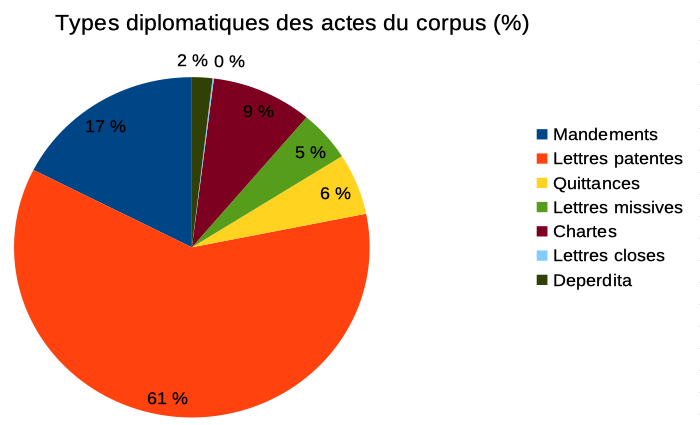
\includegraphics[scale=0.6]{img/typologie_documentaire.png}
\caption{Typologie des actes étudiés.}
\label{fig:typo_actes}
\end{figure}
\newpage 

\par  Comme le montre le graphique ci-avant, les lettres patentes sont majoritaires. Ce sont des actes à caractère juridique exprimant la volonté du duc. Ces lettres sont généralement destinées à des particuliers et beaucoup d'entre elles entérinent des nominations d'officiers, des souffrances d'hommages ou encore des donations ...\footnote{AN, P 1374\textsuperscript{2}, n° 2420 (19 février 1403) — AD Loire, B 1844, folio n°4 recto (21 mai 1453).}. Le deuxième type d'acte le plus représenté est le mandement. Ils concernent en majorité Louis II, et ce tout au long de la période\footnote{AN, P 1376\textsuperscript{2}, n° 2749 (27 février 1457) — AN, P 1389\textsuperscript{3}, n° 370 (30 juin 1410).}, et dans une moindre mesure Charles I\textsuperscript{er}\footnote{BnF, ms. fr. 20389, c. 78 (20 juin 1444).}. Ces actes ont trait à l'administration instante du duché : paiement de taxes, impositions extraordinaires, saisies, réparations diverses et fortifications, enquêtes, requêtes ...\footnote{AN, K 48, n° 6 (5 mai 1360) — AM Montluçon, AA 8 (1) (20 novembre 1360) — AM Montluçon, AA 2 (1) (1368) — AM Montluçon, n° 240, boîte 3 (7 novembre 1373) — AN, P 1376\up{2}, n° 2716 (25 août 1376) — AN, P 1379\up{2}, c. 3136/16 (18 août 1437) — AN, P 13911, c. 562 (23 mai 1447).}. Viennent ensuite les quittances et les chartes. Cette production a trait principalement aux finances (aides et paiements), à l'administration, ces deux aspects étant intimement liés, et enfin aux relations entretenues avec le roi et les autres princes. Les documents relatifs à la gestion du domaine font preuve d’une grande variété : aides, documents relatifs à l’organisation des marchés et des foires dans les localités relevant de la juridiction\footnote{AN, P 1376\textsuperscript{2}, n° 2752 (10 septembre 1366).}, et dans une moindre mesure des fondations pieuses\footnote{AN, P 1355\textsuperscript{1}, n° 46 (18 août 1392).}. Quelques mentions de trêves, d’organisation d'États ont également été relevées. Une partie de la production documentaire du duché est liée au contexte de guerre de Cent Ans : des actes mentionnent des autorisations de fortification\footnote{AD de la Loire, B 1952 (1\textsuperscript{er} mai 1435).}, des nominations de capitaines\footnote{BnF, ms. fr. 22299, folio 7 (24 octobre 1439).} et des garnisons. Les documents afférant aux relations du duc avec les grands du royaume enregistrent des alliances\footnote{AN, P 1372\textsuperscript{2}, c. 2113, (4 août 1427).}, des trêves\footnote{AD de la Côte-d’Or, B 11918, c. 117 (24 octobre 1433).}, des promesses\footnote{AD de la Côte-d’Or, B 11904, c. 67 (6 février 1436).}, mais aussi des ambassades\footnote{AN, P 1360\textsuperscript{2}, c. 881 (28 mai 1431).}, des ratifications de paix\footnote{AD du Nord, B 304, c. 15.660 (1\textsuperscript{er} octobre 1435).} ou des tractations relatives aux otages\footnote{Mention : Aubret L., Mémoires pour servir à l’histoire de Dombes, II, Guigue M.-C. (éd.), Trévoux, 1868, p. 617. Indication de provenance : \og Titres de Trévoux \fg.}. L’autre partie consiste en des ratifications de conventions de mariage\footnote{AN, P 1370\textsuperscript{2}, c. 1919 (4 février 1425).} et en paiements de dots\footnote{AD de la Côte-d’Or, B 299, pièce scellée 338 (8 décembre 1425).}. 
\newpage 

\par Malgré quelques tensions avec le roi lors de la Praguerie, Charles I\textsuperscript{er} mène une politique d’alliances par les mariages de ses enfants (Anjou, France, Bourgogne)\footnote{AN, P 1370\textsuperscript{2}, c. 1915 (14 février 1437).} et affirme sa place au rang de prince via l’écrit et la représentation. Cette production, riche et abondante, participe à la consolidation administrative qui caractérise la période. En témoigne la création des offices de gouverneur général des finances (1437) et de contrôleur général (1445)\footnote{\cite{matteoniServirPrinceOfficiers1994}}. En fin de vie, on observe une augmentation des fondations pieuses ainsi que la présence de lettres personnelles adressées à des membres de la famille, c'est notamment le cas pour le corpus d'Agnès de Bourgogne\footnote{AN, K 188, c. 304 (18 novembre 1470) — BnF, ms. fr. 15538, folio 138 (11 novembre, après 1473).}. Quelques \textit{deperdita} ont été recensés, des actes perdus ou détruits dont l'existence est attestée par une mention. Néanmoins, ils ne sont pas très représentatifs de l'ensemble du corpus puisqu'ils font en grande majorité partie du corpus de Charles I\textsuperscript{er}. Les archives des ducs de Bourbon sont progressivement versées à la chambre des comptes de Paris lors du rattachement du duché à la couronne. Une partie de ces actes a disparu dans l'incendie de la chambre des comptes de 1737, et nous est connu par des inventaires\footnote{\cite{nortierSortArchivesDispersees1965}.}. La collection de l'historiographe et collectionneur François Roger de Gaignières, donne les analyses de nombreux actes de notre corpus\footnote{BnF, ms. fr. 22388 et 22390.}. 
\newline 

\par Les actes recensés révèlent des typologies variées et offrent, malgré les pertes documentaires, un riche extrait de ce à quoi pouvait ressembler la production documentaire pour la période étudiée. Nonobstant la diversité typologique qui les caractérise, les actes émis par les ducs de Bourbon ne sont pas dépourvus de ressemblance avec les actes royaux.
\newpage 

\section[Pratiques d'\textit{imitatio regis}]{L'\textit{Imitatio regis} au c\oe{}ur des pratiques documentaires des princes de Bourbon}
\label{I.1.4}

\par Les princes du royaume de France adoptent le modèle royal en imitant les usages diplomatiques de la chancellerie royale. Même si ce modèle ne s’impose pas unanimement pour des raisons politiques (Bretagne, Bourgogne\footnote{Originalité qui va disparaître lorsque les Valois mettront la main sur le duché,  \cite{courtelChancellerieActesEudes1977}.}) ou à cause de l'usage de pratiques locales, la majorité des actes émis par les chancelleries ducales présentent de nombreuses similitudes avec les actes royaux. Olivier Canteaut relève que \og l'imitation ou le rejet des modèles sont autant d'instruments qui permettent aux autorités d’affirmer leur domination sur leurs sujets et leur identité politique face à leurs correspondants étrangers \fg\footnote{\og Introduction\fg, in : \cite{canteautDiscretLangagePouvoir2019}.}. En tant que branche cadette de la famille royale depuis le \textsc{XIII}\textsuperscript{e} siècle (descendants de Saint-Louis~(1226~-~1270)), les Bourbons bénéficient de l'office héréditaire de grand chambrier de France\footnote{Grand chambrier : grand officier de la couronne chargé de l'intendance de la chambre du roi et de la garde du trésor royal. Définition CNRTL : \url{https://www.cnrtl.fr/definition/chambrier}.} et d'une proximité particulière avec les rois de France\footnote{\og Les ducs de Bourbon, le roi et le royaume de France à la fin du Moyen Âge \fg, in : \cite{matteoniBourbonsLeurBibliotheque2022}.}. La participation de Louis II au gouvernement du royaume dès la minorité de son neveu Charles VI, ainsi que ses nombreux déplacements accompagnés de sa chancellerie, ont favorisé la circulation des conseils, des savoir-faire et des modèles\footnote{\cite{matteoniEcriturePouvoirPrincier2011}.}. La chancellerie est l’organe producteur de l'écrit princier, mais aussi de l'image et du discours du prince\footnote{\cite{generoChancellerieCharlesIer2018}.}. Celle des ducs de Bourbon, localisée à Moulins, est semblable en de nombreux points à la chancellerie royale dans son organisation, mais aussi dans la production des écrits. De plus, les \textsc{XIV}\textsuperscript{e} - \textsc{XV}\textsuperscript{e} siècles voient l'émergence et la réapparition de la figure du chancelier, l'officier chargé de l'écrit et de la garde du sceau. Il est en ce sens le responsable de la mise par écrit de la volonté politique du prince par la vérification des actes et leur signature une fois ceux-ci conformes. Olivier Guyotjeannin indique que \og se doter d’un chancelier, homme de culture juridique, rompu aux jeux du pouvoir, attiré vers la justice en ce qu’elle est le condensé du gouvernement des hommes, apparaît ainsi bien souvent comme le premier acte de l’identité diplomatique princière \fg\footnote{Conclusion par Olivier Guyotjeannin \cite{matteoniEcriturePouvoirPrincier2011}.}. Les officiers en charge de l'écrit princier sont les secrétaires, des professionnels de l'écrit public. Après délibérations du conseil ducal, et en fonction des directives de ce dernier, les secrétaires rédigent des minutes, des premières rédactions d'un acte. Les minutes sont ensuite grossoyées au propre par des clercs. La production documentaire relative à l'administration du duché de Bourbon est exécutée par des hommes qualifiés qui irriguent le milieu politico-administratif et financier bourbonnais. Ce sont majoritairement des érudits laïcs (licenciés en droit ou bacheliers en décret), dont les qualités mentionnées dans les lettres de nomination font référence à la science, à la probité, à la diligence et à la vertu\footnote{\cite{matteoniEcriturePouvoirPrincier2011}.}.  On dénombre quinze officiers chargés de l'écrit ducal sous Louis II\footnote{\cite{matteoniEcriturePouvoirPrincier2011}.} et trois chanceliers et vingt-huit secrétaires entre 1425 et 1456 (quatorze pour Charles I\textsuperscript{er} et neuf pour Agnès de Bourgogne)\footnote{\cite{generoChancellerieCharlesIer2018}.}. Ils sont généralement issus de la bourgeoisie locale, sauf quelques exceptions. Parmi elles, nous pouvons citer le cas d'Etienne de Bar, talentueux secrétaire venu de Paris, auparavant secrétaire du roi\footnote{\cite{matteoniEcriturePouvoirPrincier2011}.}. Même s'il reste isolé, ce cas de figure a pu jouer dans l'adoption des pratiques d’écriture en vigueur à la chancellerie royale.
\newline 

\par Cette pratique d'\textit{imitatio regis}\footnote{Mélissa Barry, Cléo Rager, Élisabeth Schmit, Marie-Émeline Sterlin et Clémence Lescuyer, \og \og Imitatio regis \fg ? Pour une diplomatique des actes de Jean de Berry\fg, in : \cite{guyotjeanninJeanBerryEcrit2019}.} est visible dans les écrits, au sein des caractères externes des actes. La réalisation est soignée, l'écriture conforme au modèle royal, avec des abréviations canoniques et peu nombreuses. L'organisation des différentes parties du discours suit celle des actes royaux sur un format horizontal : exposé, mentions hors teneurs, signatures organisées autour d'un paraphe cadre. Des emprunts très caractéristiques ont trait à l'ornementation avec l'utilisation de fleurs de lys, motifs typiques de l’iconographie des chartes royales contemporaines des Valois\footnote{Annexe Initiales fleurdelisées. \newline AN, P 1363\up{1}, c. 1151\up{1} (18 décembre 1448) – AN, P 1368\up{2}, c. 1628 (19 février 1447).}. Ce discours dynastique et sacré est également présent sous le principat de Charles I\textsuperscript{er}\footnote{\cite{generoSceauxArmesCharles2022}.}. On remarque des anges sur le sceau ducal et un usage plus affirmé du sceau du secret à partir des années 1440. Cette \textit{imitatio} est également manifeste dans les caractères internes des actes. Le vocabulaire de l'exposé, le contenu des clauses, la forme de la datation ainsi que la notification \og a tous présens et a venir \fg \space ou \og a tous ceux qui ces presentes verront \fg \space témoignent d'une proximité importante avec la chancellerie royale. L'organisation des parties du discours et le vocabulaire suivent ceux en usage à la cour du roi de France. Néanmoins, quelques dissemblances peuvent être relevées. Les différences majeures se rapportent aux verbes usités et à la langue des actes. En Bourbonnais, la langue vernaculaire domine. Les quelques actes rédigés en latin sont généralement des actes très solennels destinés aux clercs et aux institutions religieuses. 
\newline
\par La structuration de la chancellerie sous Louis II et sa prolongation sous Charles I\textsuperscript{er} marque un approfondissement de l'\textit{imitatio regis} qui traduit l'attachement familial des Bourbons au lignage des rois de France et une volonté d'asseoir leur pouvoir par l'imitation du modèle royal. Le rôle des individus, notamment des officiers de la chancellerie, est également à souligner dans la diffusion des pratiques d’écriture pour la période étudiée. 
\newline 
\newline 
\par Le corpus rassemble des actes princiers aux typologies variées, dispersés au gré des différentes institutions de conservation et s'échelonnant sur une période de plus d'un siècle. La production recensée qui a permis de former le corpus étudié est le fruit d'un travail de longue haleine de regroupement puis d'édition des actes. 

\newpage
\thispagestyle{empty}
\mbox{}
\newpage
 
	\chapter[Éditions numériques]{Des éditions numériques à partir d'un logiciel de traitement de texte}

\vspace*{\stretch{1.3}} 
\par Les premiers projets d'édition sont impulsés par des érudits au \textsc{XIX}\textsuperscript{e} siècle, avec comme objectif principal de rassembler des corpus et d'en fournir les éléments d'analyse\footnote{\og L'évolution des pratiques éditoriales \fg, in : \cite{guyotjeanninConseilsPourEdition2009}.}. Les actes des princes laïcs sont quelque peu délaissés par ces entreprises au profit des actes pontificaux et royaux. Les perspectives qu'offre aujourd'hui le numérique permettent l'étude de corpus importants et dispersés sur un temps indéterminé, autant de possibilités que n'offre pas la publication d'un ouvrage, comprenant ainsi la reproduction, la publication et la diffusion de documents d'archives. C'est dans ce contexte que l'on voit se développer des entreprises d'édition consacrées aux actes princiers et dans lequel s'inscrivent les éditions des actes émis par les Bourbons. 
\vspace*{\stretch{0.7}} 
\newpage 

\section{Trois projets d'édition}
\label{I.2.1}

\vspace*{\stretch{0.1}} 
\par Les quatre corpus rassemblant les actes de Louis II, d'Anne Dauphine, de Charles I\up{er} et d'Agnès de Bourgogne sont stockés, au commencement du stage sur lequel ce mémoire s'appuie, dans des fichiers de traitement de texte. Ces fichiers ont été constitués à l'issue du travail de recensement des actes dans les différentes institutions citées précédemment. Il s'agit d'éditions critiques : des éditions spécifiques qui collationnent les variantes d’un texte tout en pourvoyant ce dernier d’un apparat critique\footnote{L'apparat critique désigne l'ensemble des annotations d'érudition qu'un éditeur ajoute à un texte original. \og Le destin de l'appareil critique dans l'édition scientifique numérique\fg, in : \cite{apollonEditionCritiqueEre2017}.}. 
\newline 

\par Ces éditions ont été menées par plusieurs chercheurs, sur des temporalités différentes et avec des objectifs différents : recherches personnelles, mémoire académique et travail préparatoire d'une communication scientifique. Les actes de Louis II ont été édités par Olivier Mattéoni, enseignant chercheur à l'Université Paris 1 Panthéon-Sorbonne, dans le cadre de ses recherches sur les Bourbons\footnote{\cite{matteoniEcriturePouvoirPrincier2011}}. Il a notamment soutenu une thèse de doctorat sur les officiers bourbonnais en 1994 et publié de nombreux travaux sur le duché et les ducs de Bourbon\footnote{\cite{matteoniServirPrinceOfficiers1994}.}. Les actes de Charles I\up{er} et d'Agnès de Bourgogne ont été édités par Jean-Damien Généro pour son mémoire de Master recherche soutenu à l'Université Panthéon-Sorbonne en 2018, sous la direction d'O. Mattéoni\footnote{\cite{generoChancellerieCharlesIer2018}.}. Les actes d'Anne Dauphine ont enfin été édités conjointement par O. Mattéoni et J.-D. Généro en vue de présenter une communication sur la diplomatique de la duchesse au colloque organisé en 2017 pour les cinq cents ans de sa mort\footnote{\cite{matteoniActesAnneDauphine2019}.}.O. Mattéoni a par la suite retravaillé les fichiers de Louis II et d'Anne Dauphine en systématisant l'ajout des notes critiques qui concernent les individus et les lieux. Il a aussi rédigé de succinctes biographies des individus qui apparaissent régulièrement dans les actes (les grands officiers, les grands prélats) et les a ajoutées comme note critique à chaque fois que ces individus apparaissent. Pour les lieux, il a précisé leurs localisations (toponyme actuel, canton, département). Dans la mesure où il n'est pas possible de prévoir comment les utilisateurs vont aborder le corpus sur le site internet ni quel sera soit leur point d'entrée, l'existence de notes concernant les individus et les lieux demeure essentielle. 

\par Les éditions des actes de Louis II et d'Anne Dauphine n'étaient pas destinées à être immédiatement éditées sous forme papier ou électronique, tandis que celles des actes de Charles I\up{er} et d'Agnès de Bourgogne ont été imprimées dans le cadre d'un travail universitaire. Ces finalités différentes supposent des choix de mise en forme et de mise en page différents, qui ont une influence sur les traitements postérieurs. En effet, concevoir un fichier de traitement de texte dans le but de l'imprimer implique de privilégier les aspects visuels de l’édition et sa mise en page.

\par Les actes ont été édités grâce à un logiciel de traitement de texte. Le traitement de texte qualifie les logiciels qui permettent à un utilisateur de rédiger du contenu informatisé. Ces logiciels sont multiples et utilisent différents formats (ODT, docx) plus ou moins compatibles selon les logiciels et les systèmes d'exploitation. Un format de fichier spécifie la manière dont les données sont stockées pour une application particulière \footnote{Microsoft, \og En apprendre plus sur les formats de fichiers\fg, \url{https://support.microsoft.com/fr-fr/office/en-apprendre-plus-sur-les-formats-de-fichiers-56dc3b55-7681-402e-a727-c59fa0884b30}.}. La lecture des différents formats et de leur mise en forme diffère selon les applications. J.-D. Généro a édité les actes de de Charles I\up{er} et d'Agnès de Bourgogne sur le logiciel de traitement de texte \textit{Pages} de MacOS avant de les convertir en ODT. Les actes d'Anne Dauphine ont également été édités sur un fichier ODT tandis que les actes de Louis II ont été édités sur un fichier docx. Le fichier docx est un document Microsoft Word au format Open XML et le fichier ODT est un document LibreOffice au format OpenDocument. Même si OpenDocument Format (ODF) prend en charge les fonctionnalités OpenOffice et Open XML, et que Microsoft Office prend en charge ODF, toutes les fonctionnalités ne sont pas prises en charge, ce qui peut occasionner des changements en termes de modification d’un document et des pertes de contenu.

\par Les travaux de recherche, même à leurs prémisses, sont rarement neutres, puisque les données ne le sont pas non plus, et qu'ils consistent en la reprise de données qui ont souvent déjà été traitées. Les fichiers de traitement de texte peuvent être qualifiés de \textit{legacy data}, puisqu'ils sont le résultat de traitements antérieurs opérés par les premiers chercheurs à travailler sur le corpus\footnote{Sur le concept de \textit{legacy data}, voir : \cite{reignierVersIndexationAutomatique2022}.}. Les ingénieurs du projet \og Actes princiers\fg \space ont conscience qu'ils vont devoir composer avec cela tout au long de leurs traitements et intégrer ce paramètre à leur réflexion.
\newline 

\par Ces différences de finalités et de formats posent des problèmes d'harmonisation des données lorsqu'il s'agit de regrouper les actes des ducs de Bourbon pour en proposer une édition cumulative. Malgré ces disparités dans la mise en page, les éditions comportent des similitudes, notamment dans leurs présentations que l'on peut qualifier de diplomatiques.
\newpage

\section{Des éditions diplomatiques}
\label{I.2.2}

\par Les différentes éditions suivent les normes en vigueur développées dans les \textit{Conseils pour l'édition des textes médiévaux} de l'École Nationale des Chartes\footnote{\cite{guyotjeanninConseilsPourEdition2014}. - \cite{guyotjeanninConseilsPourEdition2009}.}, inspirés des règles établies en 1984\footnote{\cite{c.i.d.NormesInternationalesPour1984}.}. Les actes médiévaux étant généralement écrits d'un seul bloc, il est d'usage de restituer cette mise en forme en éditant le contenu textuel de l'acte en un seul paragraphe. Le texte édité est accompagné d'éléments de présentation. Comme l'explique Olivier Guyotjeannin, \og une fois le texte établi et son apparat mis en forme, il reste à le munir d'un "habillage", composé des éléments de présentation qui guideront la lecture. L'éditeur cherche à concilier le respect d'éléments qui peuvent être signifiants et les commodités fournies au lecteur contemporain \fg \footnote{\og La présentation de l'édition \fg, in : \cite{guyotjeanninConseilsPourEdition2009}.}. 
\newline 

\begin{figure}[ht]
\centering
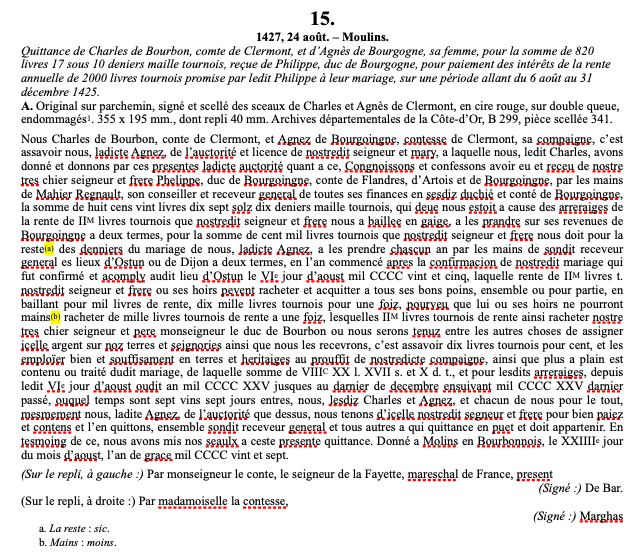
\includegraphics[scale =0.6]{img/edition.png}
\caption{Édition diplomatique de l'acte daté du 27 août 1427.}
\label{fig:ed_diplo}
\end{figure}

\newpage 

\par Comme nous pouvons le voir dans l'exemple ci-avant, chaque acte est précédé d'un numéro d'ordre permettant de le situer dans le corpus. Viennent ensuite les dates de temps et de lieu. 
\newline 

\par La date de temps est restituée sous une forme contemporaine et débute par l'inscription du millésime, suivi du quantième et du mois. Dans le cas où le millésime convertit par l'éditeur viendrait à différer de celui indiqué dans l'acte, en raison du style en vigueur chez les contemporains, ce dernier est suivi de la mention (n.st.). En effet, la chancellerie des ducs de Bourbon suivant le style de Pâques, il est nécessaire de convertir les dates ayant lieu avant cette fête en style du premier janvier. Si la date a été reconstituée, les adverbes de temps \og avant \fg \space et \og après \fg \space sont précisés en amont. 
\newline 

\par La date de lieu est séparée de la date de temps par un point, un blanc et un tiret et les toponymes sont restitués selon leur forme actuelle s'ils ont pu être identifiés. 
\newline 

\par Une analyse (regeste) précède le texte édité afin d'en proposer un résumé et d'en préciser la typologie. Elle est indiquée en italique et se doit être la plus efficace possible dans la compréhension de l'acte qu'elle va offrir au lecteur. 
\newline 

\par L'analyse est suivie d'un tableau de la tradition qui indique l'état de la tradition et mentionne les différents témoins ayant permis l'établissement du texte. Ce tableau commence par une description de l'original, dans le cas où il est existant, qui comporte les mentions de son support (parchemin, papier), de sa forme (rouleau, cahier~...), de ses dimensions (en millimètres), du mode de scellage, de son état de conservation ainsi que l'institution où il est conservé. Cette mention est suivie de celle des autres témoins, généralement des copies pour lesquelles on précise la nature juridique (copie d'après original, vidimus ...), la date, l'auteur, le recueil dont elle est tirée ou la source. Les éditions sont également mentionnées, notamment dans le cas des \textit{deperdita}. 
\newline 

\par Le corps du texte suit ces éléments d'identification et de précision. Il est annoté via un apparat critique fournissant des renseignements liés à l'établissement du texte (choix d'édition : variantes, remarques ...) et une annotation historique apportant des précisions utiles à la compréhension du texte\footnote{\og La mise au point du texte\fg, in \cite{guyotjeanninConseilsPourEdition2009}}. Lorsque l'on édite des originaux, la localisation des signatures et des mentions hors teneurs dans l'espace graphique du parchemin est précisée, généralement en dessous du texte. Le nom de signataires est signalé en petites capitales et précédées de la mention \og (Signé :)\fg. Les mentions hors teneurs sont également précédées de mentions \og (Sur le repli :)\fg \space ou \og(Sous le repli :)\fg, selon les cas. Dans le cas où elles sont nombreuses, des précisions sur leur disposition peuvent être indiquées : \og(À gauche :)\fg ~...

\par En dépit des recommandations canoniques pour la production d'éditions diplomatiques, les pratiques d'édition des deux chercheurs sont différentes. C'est le cas pour les notes de bas de page, qui ont été placées à la suite de l'acte auquel elles faisaient référence pour les éditions des actes de Louis II, et insérées à partir d'une fonction disponible sur ODT pour les autres éditions. Le corpus de Louis II est également le seul dont les actes ne comportent pas de numérotation. Même si cette dernière peut être questionnée lors de la découverte de nouveaux actes, elle participe à la structuration du corpus. 
\newpage 

\section{Le traitement de texte : un bon compromis ?}
\label{I.2.3}

\par L'édition à partir d'un logiciel de traitement de texte n'est pas sans avantages. Contrairement à une édition papier imprimée, elle n'est pas figée. L'intégration progressive des données au fur et à mesure de l'avancée des travaux de recherche est possible, là où une édition imprimée ne permet pas ces mises à jour, ou alors via des publications additionnelles\footnote{Canteaut, Olivier, Moufflet, Jean-François, \og Les éditions d'actes princiers (\textsc{XII}\up{e} - \textsc{XV}\up{e} siècle) : bilan à l'ère du numérique \fg, in : \cite{guyotjeanninJeanBerryEcrit2019}}. Ces fonctionnalités sont particulièrement utiles dans le cadre d'éditions diplomatiques, dans la mesure où elles permettent, lors de la découverte de nouveau états du texte, de les ajouter au corpus. Néanmoins, le traitement de texte ne permet pas le remplissage automatique des données contrairement à d'autres technologies comme Python. Même s'il permet l'intégration de nouveaux actes, celle-ci doit se faire manuellement. Cela nécessite de réfléchir en amont à la structuration la plus adaptée possible de son édition, pour éviter d'avoir des problèmes lors de l'ajout de nouvelles données. 
\newline 

\par Prenons le cas du corpus de Charles I\textsuperscript{er} dans lequel les actes sont numérotés un à un. Quid de cette numérotation lors de l'intégration d'actes inédits au corpus ? Lors de notre visite aux Archives nationales en avril 2023, nous avons photographié cinq actes inédits repérés par O.~Mattéoni dans la série P\footnote{AN, P 452\up{2}, c. 190 (24 octobre 1443) - AN, P 452\up{2}, c. 307 (24 octobre 1443) - AN, P 452\up{2}, c. 313 (24 octobre 1443) - AN, P 452\up{2}, c. 229 (25 octobre 1443) - AN, P 452\up{2}, c. 169 (22 octobre 1454).}. Nous avons décidé de les intégrer à un CSV (comma-separated values)\footnote{Type de fichier spécial dont les valeurs sont séparées par des virgules et qu’il est possible de créer ou de modifier dans Excel, définition in : Microsotf, \og Créer ou modifier des fichiers .csv à importer dans Outlook\fg, \url{https://support.microsoft.com/fr-fr/office/cr}.} répertoriant les informations des actes. Néanmoins, cela a ensuite posé des problèmes de correspondance des données, car la numérotation ne correspondait plus une fois ces actes intégrés au corpus. La question de leur intégration immédiate au corpus s'est donc posée et il a été décidé de les intégrer postérieurement dans le projet. C'est pourquoi réfléchir à un schéma, à des pratiques d'édition communes, facilite le travail conjoint de plusieurs chercheurs sur un même corpus. 
\newline 

\par L'édition numérique ou électronique désigne une édition mise en forme et diffusée dans un environnement numérique. L'édition des actes sur un logiciel de traitement de texte peut en ce sens être vue comme une édition numérique dans la mesure où elle peut être lue sur un écran. De plus, à l'instar de l'édition numérique, elle laisse la possibilité aux ajouts, aux corrections ainsi qu'à l'élargissement du corpus. Ces mêmes ajouts et corrections peuvent être le fait différents contributeurs. Le travail peut également être fractionné en fonction des spécialités de chacun (transcription, mise en forme ...)\footnote{\cite{apollonEditionCritiqueEre2017}.}. Néanmoins, l'ambition principale d'une édition numérique n'est pas sa lecture seule, mais son accessibilité. Celle-ci est permise par la mise en ligne des données, qui offre des fonctionnalités supplémentaires contribuant à renforcer la souplesse et la qualité de l'édition.
\newline 

\par La mise en ligne des données, soit leur disponibilité et leur accessibilité sur un réseau, permet un certain nombre de possibilités qui ne sont pas à négliger dans le cadre d'une édition de textes médiévaux. Elle propose des interfaces de consultation et de visualisation qui mettent considérablement en valeur le projet. La mise en page est améliorée et offre une meilleure lisibilité au lecteur. C'est notamment le cas avec l'apparat critique, qui peut vite entraver la mise en page dans le cas d'une édition papier ou à partir d'un logiciel de traitement de texte\footnote{\og Le destin de l'appareil critique dans l'édition numérique scientifique\fg, in : \cite{apollonEditionCritiqueEre2017}}. L'hébergement en ligne permet des notes interactives et un certain nombre de renvois aux références sans avoir recours à des notes de bas de page qui alourdissent l'édition et qui nécessitent parfois de faire des choix sur les informations communiquées au lecteur. La présentation est dans l'ensemble plus complexe et offre un affichage multiple avec plusieurs vues du texte : affichage des autres états et des variantes (possibilité d'afficher un fac-similé via un hyperlien). Les traductions et les transcriptions peuvent être affichées de manière interactive\footnote{C'est par exemple le cas des dossiers documentaires du THELEME. \cite{TechniquesPourHistorien}.}. La mise en ligne permet également une publication progressive des recherches, et offre une disponibilité de ce qui a déjà été traité pour la communauté scientifique, mais aussi pour un public plus large (généalogistes...). Une édition dynamique interactive rend le travail d'édition pilotable par l'utilisateur, permettant ainsi plus de possibilités et une réflexion sur le travail d'édition\footnote{\cite{apollonEditionCritiqueEre2017}}. Le lecteur a aussi la possibilité de filtrer les informations et les métadonnées essentielles à ses travaux de recherche. 
\newline 

\par Malgré des choix d'édition proches, le logiciel de traitement de texte permet de trop nombreuses variations et ambiguïtés selon le format utilisé. Ces variations posent des problèmes d'harmonisation qui ne seront pas sans conséquence lorsque se posera la question de l'accessibilité des données. En effet, l'accès aux données à la communauté scientifique est l'une des fins, pour ne pas dire la fin, du travail d'édition. Cette accessibilité est aujourd'hui largement facilitée et augmentée par la mise en ligne des travaux. L'ODT offre un compromis relativement simple à prendre en main, mais dont les possibilités d'interopérabilité\footnote{L'interopérabilité désigne la capacité de systèmes, unités, matériels à opérer ensemble.} et de structuration des données nécessaires aux travaux d'édition de corpus conséquents sont vite limitées. L'harmonisation des éditions est donc primordiale et passe par le choix d'outils (automatiques ou manuels) plus adaptés et intéressants pour la recherche, offrant des possibilités de manipulation des données plus élevées.

\newpage
\thispagestyle{empty}
\mbox{}
\newpage


	
	\part{Du traitement de texte à l'encodage} 

\chapter[Préparation à l'encodage]{Préparer le traitement de texte à l'encodage en XML}

\vspace*{\stretch{1.3}} 
\par Les actes du corpus étant édités aux formats ODT et docx, il s’agit dans un premier temps de les nettoyer, c’est-à-dire de les préparer à un encodage, afin de permettre aux chercheurs de manipuler le corpus. XML (Extensible Markup Language) est un langage de balisage qui révèle la structure et la sémantique des données, conçu pour la description des documents textuels, et en ce sens adapté pour l'édition critique. Le recours au langage de balisage XML permet une structuration des éléments textuels à l'aide de balises, ce que le traitement de texte ne permet pas. Depuis 1998, XML est un langage libre et documenté qui facilite la lisibilité des données, leur échange et leur migration vers d’autres plateformes, logiciels et formats. C'est aujourd'hui un standard du W3C\footnote{World Wide Web Consortium : communauté internationale qui développe des normes ouvertes pour assurer la croissance à long terme du Web.} qui comporte différents formats comme la TEI (Text Encoding Initiative) pour l'encodage de documents patrimoniaux.
\vspace*{\stretch{0.7}} 
\newpage 

\section{Le recours à un langage de balisage}
\label{II.3.1}

\par Le chercheur en philologie Claus Huitfeld défini le balisage comme \og l'usage de chaînes de caractères réservés, insérées dans des séquences de caractères dans des fichiers de documents numériques, afin de dénoter ou de signaler des caractéristiques d'un document qui ne peuvent pas être transmises par des caractères représentant directement leur contenu verbal \fg \footnote{\og Systèmes de balisage de textes et édition critiques\fg, in : \cite{apollonEditionCritiqueEre2017}}. Le terme balisage renvoie à des marqueurs spéciaux permettant de signaler certaines propriétés du document numérique (ponctuation, notes…) via un ensemble de balises\footnote{\cite{apollonEditionCritiqueEre2017}}. L’édition scientifique actuelle fait appel à des méthodes de publication informatisées qui induisent du balisage. Les systèmes de traitement de texte ou de publication sur le web les plus utilisées actuellement disposent d’un système de balisage en \og arrière-plan \fg \space que l'usager n'a pas à gérer : il intervient directement sur le document via une mise en page visuelle (WYSIWYG : \og what you see is what you get \fg\footnote{\og Ce que vous voyez est ce que vous obtenez\fg : l'utilisateur voit directement le résultat de sa saisie.}). Ces outils sont utiles pour l'affichage à l'écran ou l'impression papier, mais dès lors que l'on souhaite proposer des outils de recherche performants, de comptage, ou encore d'analyse, il devient nécessaire d'effectuer un balisage généralisé du texte. Différents langages de balisage existent et comprennent une syntaxe, un vocabulaire contrôlé, des méthodes, des pratiques et des outils associés\footnote{\og Systèmes de balisage de textes et édition critiques\fg, in : \cite{apollonEditionCritiqueEre2017}}. 
\newline 

\begin{figure}[ht]
    \centering
    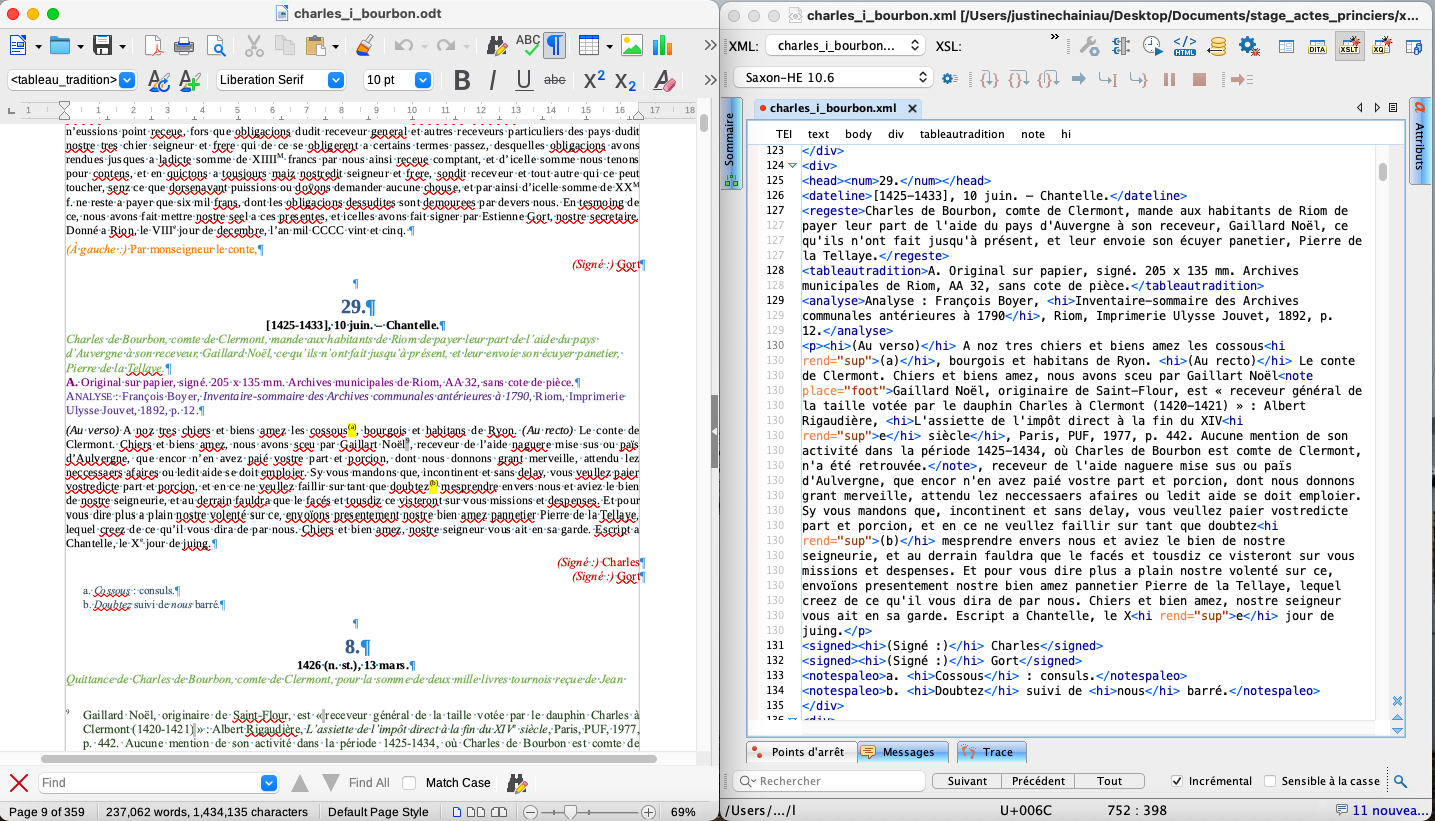
\includegraphics[scale=0.3]{img/odt_vs_xml.png}
    \caption{Traitement de texte et encodage de l'acte n°29 daté du 10 juin 1425-1433.}
    \label{fig:odt_vs_xml}
\end{figure}
\newpage 

\par Le langage XML est le plus approprié pour l’édition numérique. Contrairement au langage HTML (HyperText Markup Language) dont les balises définissent l’apparence des données (titres, paragraphes), les balises du langage XML définissent la structure et la signification sémantique des données, ce qui permet leur réutilisation. La particularité du XML est que son affichage nécessite une interprétation, soit une transformation du document. Le document XML est alors transformé via des feuilles de style XSL (Extensible stylesheet language)\footnote{Extensible stylesheet language : langage des feuilles de style associées à XML.} en document HTML pour une disponibilité sur le web ou en PDF pour une impression de qualité. Cette possibilité de présentation dans une variété de formats sans qu'il soit nécessaire de modifier le code assure l'intégrité des données. En effet, la conversion d'un document produit sous traitement de texte peut être difficile, manquer de fiabilité. De plus, les formats propriétaires ne sont pas documentés publiquement (usage commercial) et comportent un risque d’obsolescence qu’il est important de prendre en compte lorsque l’on souhaite produire un travail pérenne. Ainsi, l’un des principaux avantages du balisage généralisé est son interopérabilité, qui garantit une utilisabilité future. Dans le cadre de la recherche en sciences humaines et sociales, de l’édition en particulier, il est primordial de faciliter l'échange et la réutilisation des documents numériques et d’assurer leur conservation sous une forme qui les rend accessibles à la recherche. Un autre avantage du balisage généralisé est son adaptabilité à différents projets d'édition. Pour cela, différents langages XML ont été développés. 
\newline 

\par En 1994 sont publiées les Recommandations méthodologiques pour le balisage et l'échange de textes électroniques de la TEI\footnote{Text Encoding Initiative : consortium qui élabore et maintient collectivement une norme pour la représentation des textes sous forme numérique : \url{https://tei-c.org/}.}, soit un ensemble de balises qui peuvent être combinées et adaptées à des besoins spécifiques\footnote{\og Systèmes de balisage de textes et édition critiques\fg, in : \cite{apollonEditionCritiqueEre2017}}. La TEI est un langage descriptif de balisage adapté à la description fine des différents aspects d’une source, permettant ainsi au chercheur de caractériser les informations utiles à la production d'une édition. Il s'agit d'un ensemble de recommandations pour les chercheurs sur la création de ressources textuelles informatisées et lisibles par des machines, adaptées aux besoins de la recherche et extensibles, puisque ces besoins changent et évoluent\footnote{\cite{burnardQuEstceQue2015}.}. Les Guidelines de la TEI définissent plusieurs centaines de concepts différents permettant une description scientifique et sémantique d’un texte pour des projets d'édition variés (théâtre, poésie, documents d'archives...). 
\newpage 

\par Les technologies de balisage adaptées à l’édition numérique rendent possible la séparation entre la description et la présentation. Cette différenciation entre la transcription des données textuelles et leur présentation offre à l'éditeur la possibilité de développer de manière distincte l’enregistrement du document et l’affichage des données et des métadonnées le caractérisant (notes, index…)\footnote{\og Éditions critiques et séparation de la description et de la présentation, in : \cite{apollonEditionCritiqueEre2017}}. La technologie remet donc en question les pratiques traditionnelles de l'édition. Les standards de balisage du texte assurent l’interopérabilité des données, contribuent à améliorer la qualité de l'édition et de ses éventuelles révisions, et sont en ce sens novateurs. Toutefois, les langages de balisage nécessitent de se familiariser avec leur syntaxe, ce qui peut parfois motiver le choix d’une édition via un logiciel de traitement de texte, comme dans notre cas. 
\newline 

\par Deux possibilités d'encodage s'offrent désormais à nous pour transformer le corpus : manuelle ou automatique. L'encodage manuel étant chronophage, la conversion automatique est plus appropriée. Toutefois, la conversion des ODT en XML sans opérations préparatoires risque de générer une \og dette technique \fg \space (maintenances qui auront une incidence importante sur l'ensemble du projet). En effet, parmi les opérations de traitement des XML obtenus, certaines auraient pu être évitées si la mise en forme du document ODT d'origine avait été améliorée. Pour pallier cette \og dette\fg, il est nécessaire d'harmoniser au maximum les documents en amont.

\newpage 

\section[Utilisation de regex]{Utilisation de regex pour une première structuration du texte}
\label{II.3.2}

\vspace*{\stretch{0.1}} 
\par Le recours à des expressions régulières (regex)\footnote{\cite{ListRegularExpressions}.} s’est révélé opportun pour automatiser le nettoyage des documents\footnote{\cite{UsingRegularExpressions}.}. Les regex sont des chaînes de caractères utilisées pour décrire, dans une syntaxe précise, un ensemble de chaînes de caractères possibles. Leur emploi peut être exécuté à partir de la fonction rechercher/remplacer du traitement de texte. Elles peuvent également être utilisées pour rechercher des caractères non spécifiés ou même invisibles (espaces, sauts de lignes...). Le corpus des actes émis par Agnès de Bourgogne étant moins volumineux, il a tenu lieu d’expérimentation afin de tester la pertinence des regex et leur prochaine application au corpus plus important que représentent ceux de Louis II et de Charles I\textsuperscript{er}. 
\newline 

\par L’utilisation de regex simples a permis dans un premier temps de parfaire la mise en page du document en retirant les doubles espaces, les sauts de lignes ou encore les pages inutiles\footnote{Annexe Liste des regex utilisées.}. Cette étape a été exécutée avec facilité pour le premier corpus relatif aux actes d’Agnès de Bourgogne. Néanmoins, le traitement d’un fichier plus volumineux, comme celui de Charles I\textsuperscript{er}, nous confronte à des problèmes de mise en page. Nous remarquons la présence d’espaces similaires à des tabulations devant les mentions hors teneurs. L’affichage de \og la mise en page \fg \space sur Word a permis de repérer ces anomalies, à savoir l’apparition de mentions \og sur le repli \fg \space par la suite masquées en blanc afin d’aligner les mentions hors teneur en vue de l'impression du mémoire de Master. Le recours à une regex plus ciblée a permis leur suppression et a réglé les problèmes d’indentation. Dans un second temps, les regex ont contribué à améliorer la lisibilité du document. Les notes paléographiques ont bénéficié d’un retour à la ligne et les astérisques faisant office de séparateur des actes ont été supprimées. Seule la numérotation des actes a été retenue, car contrairement aux astérisques, elle est présente dès le premier acte, ce qui évitera un encodage manuel de ce dernier, permettant ainsi d'automatiser totalement le processus. 
\vspace*{\stretch{0.2}} 
\newpage 

\par L'automatisation du nettoyage des données via des regex s’est révélée être une méthode puissante pour uniformiser rapidement les éditions. Néanmoins, certaines étapes du nettoyage ont dû être effectuées manuellement, afin d'éviter une perte de données. C’est le cas tout au long du travail avec les fautes orthographiques qui peuvent être repérées progressivement. Les notes de bas de page présentes dans les dates ont été déplacées à la fin de l'analyse afin d'éviter de surcharger l'encodage. Certaines erreurs trop volumineuses n’ont pas encore été résolues et nécessitent un questionnement. C’est le cas de la présence aléatoire de points à la suite des dates. Il y a aussi des problèmes d’harmonisation des mentions hors teneurs et des signataires qui ne sont parfois pas signalés en amont, ce qui ne permet pas de les identifier et d'intervenir dessus via des regex. 
\newline 

\par Ces deux premières étapes n’ayant pas permis de résoudre tous les problèmes de mise en page et d’uniformisation, les dernières phases du processus auront lieu plus tardivement dans le projet lors de l’utilisation d’autres technologies. La mention \og (Signé :) \fg \space devant le nom de chaque signataire n’étant pas continue, il sera plus simple de l’ajouter ou de la retirer plus tardivement lors de l'encodage en XML à partir d'un script Python. Le nettoyage des données découle donc des différentes phases du projet et est aussi dépendant des formats (ODT, XML) et des technologies utilisées (Python...), même si des étapes peuvent être pensées afin de préparer les données à une conversion.

\newpage 

\section[Proposition de stylage]{Proposition de stylage des actes en vue d’une conversion}
\label{II.3.3}

\par Les logiciels de traitement de texte permettent d'appliquer des styles différents à des parties du texte. Le recours aux regex s'est avéré efficace pour structurer le texte via le stylage des différentes parties des éditions. Un style est un \og ensemble de règles de mise en forme, regroupées, nommées, hiérarchisées et enregistrées, afin de pouvoir être facilement réutilisées en bloc par la suite \fg\footnote{Open Office, \og Utiliser Styles et Modèles
avec OpenOffice.org\fg.}. Ces derniers offrent à l'utilisateur un contrôle de la mise en forme des documents. Le format OpenDocument est une archive ZIP contenant des fichiers XML qui renferment le contenu du document (content.xml), les styles utilisés (styles.xml) et les métadonnées associées au fichier (meta.xml)\footnote{Microsoft, \og Différences entre le format Texte OpenDocument (.ODT) et le format Word (.docx)\fg, \url{https://support.microsoft.com/fr-fr/office/diff}.}. Ainsi, lors de la transformation des documents ODT vers XML, les différents styles associés aux parties des éditions seront interprétés par l’éditeur de code, ce qui permettra de les distinguer dans des balises structurantes. 

\par Toutes les différentes parties des éditions : datation, analyse, tableau de la tradition, mentions hors teneurs, signataires, notes paléographiques et notes de bas de page ont été stylées via des regex\footnote{Annexe Liste des regex utilisées.}. Dans la mesure où la mise en forme de toutes ces parties était relativement normalisée, les expressions régulières ont permis d'identifier les chaînes de caractères ciblées et de les styler. Les styles ont été créés à l'aide de la fenêtre flottante \og Styles et formatage \fg \space qui permet de visualiser les différents styles, de les utiliser, de les modifier, d’en créer ou d'en supprimer. Ces styles ont ensuite été réutilisés et appliqués aux autres documents ODT pour les actes de chaque prince. Nous avons opté pour un stylage coloré afin d'avoir un meilleur aperçu des différentes parties des éditions visuellement. Comme le montre les différents exemples ci-après, le stylage n'a pas été appliqué aux mêmes parties de l'édition selon l'état des actes. Les originaux sont les actes qui ont demandé le plus de stylage dans la mesure où ils comportent toutes les parties de l'édition. 

\begin{figure}[H]
    \centering
    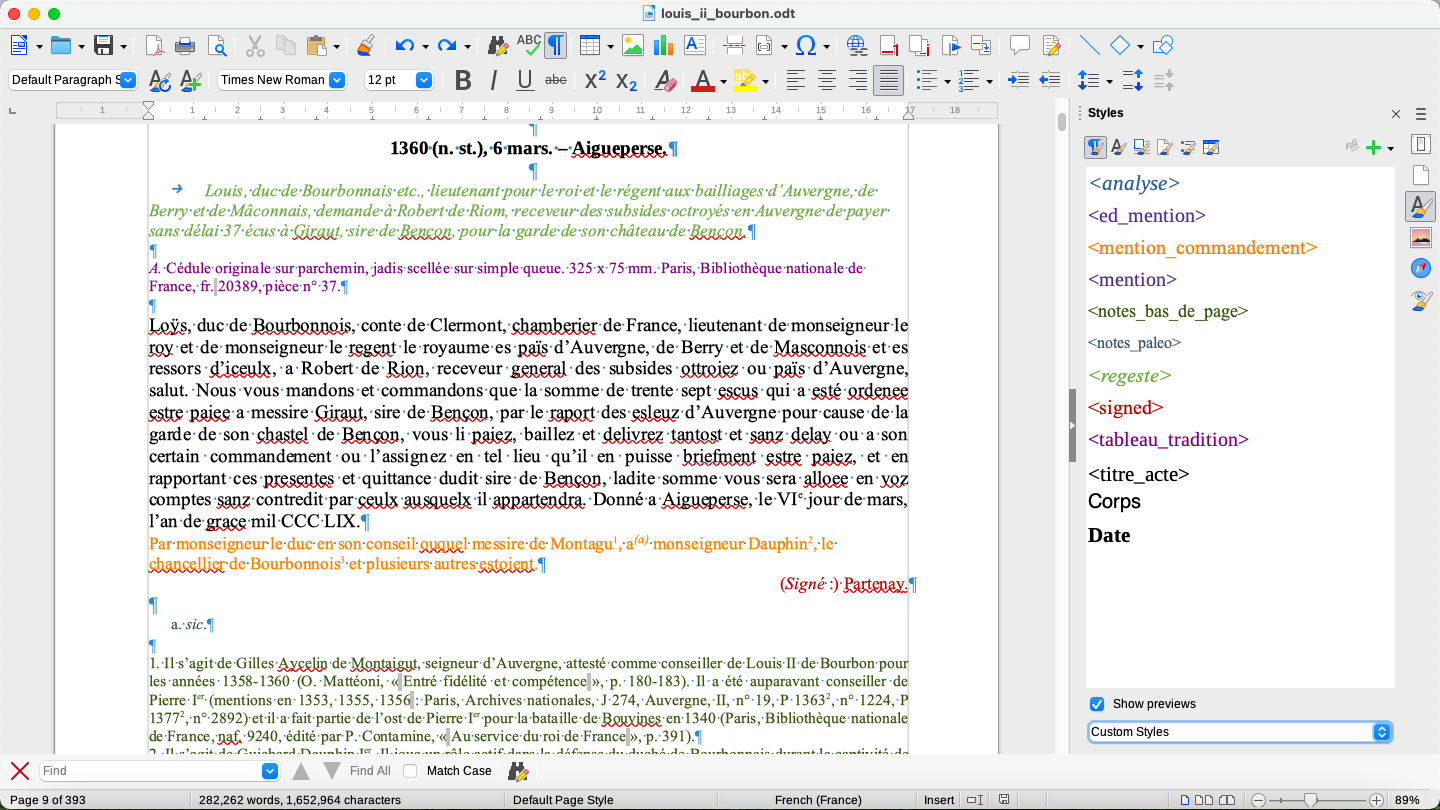
\includegraphics[scale=0.3]{img/original.png}
    \caption{Original daté du 6 mars 1360.}
    \label{fig:original}
\end{figure}

\begin{figure}[H]
    \centering
    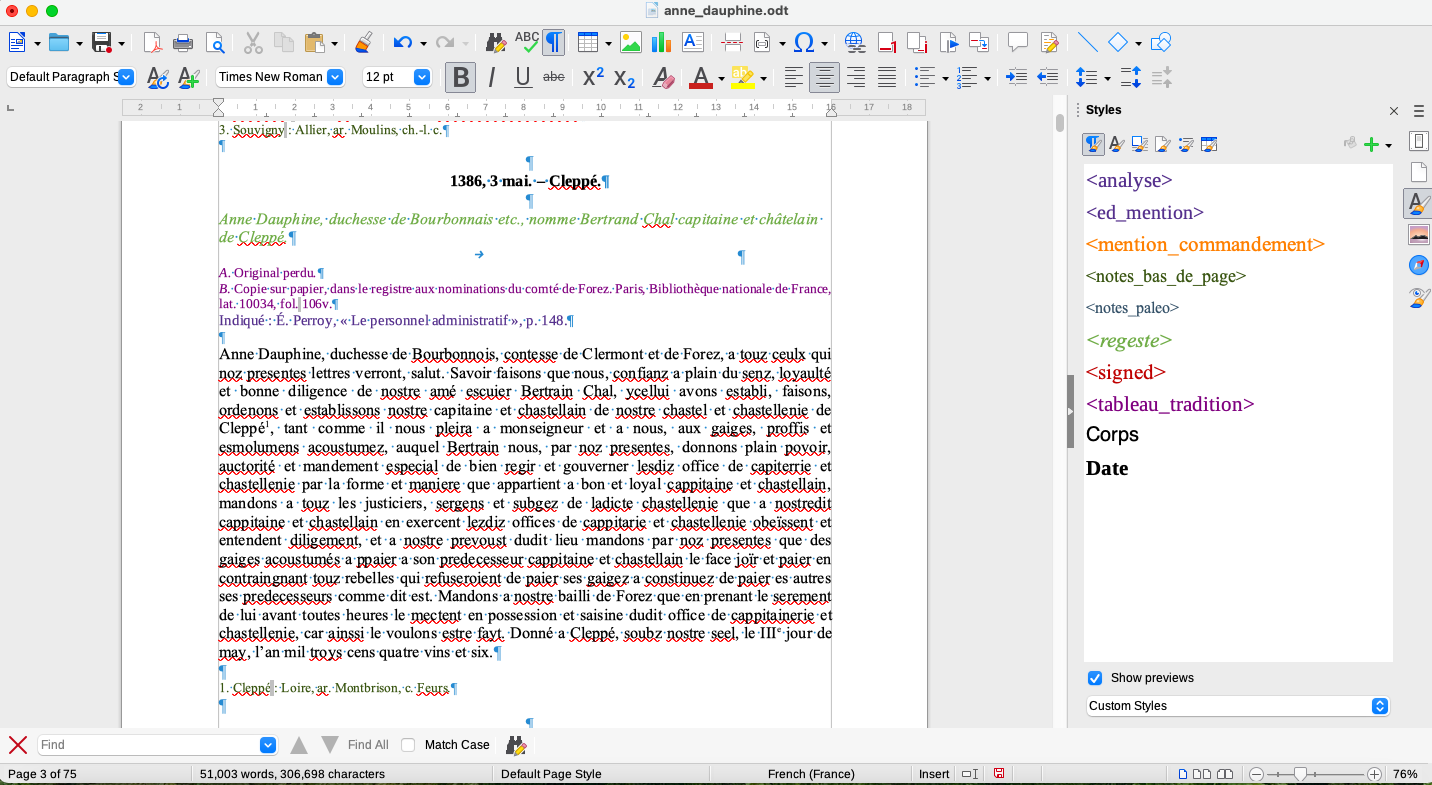
\includegraphics[scale=0.3]{img/copie.png}
    \caption{Copie datée du 3 mai 1386.}
    \label{fig:copie}
\end{figure}

\par Les copies et vidimus ne comportent pas de stylage pour les mentions hors teneurs et les signataires puisque l'acte copié ou vidimé est présenté d'un bloc. 

\begin{figure}[H]
    \centering
    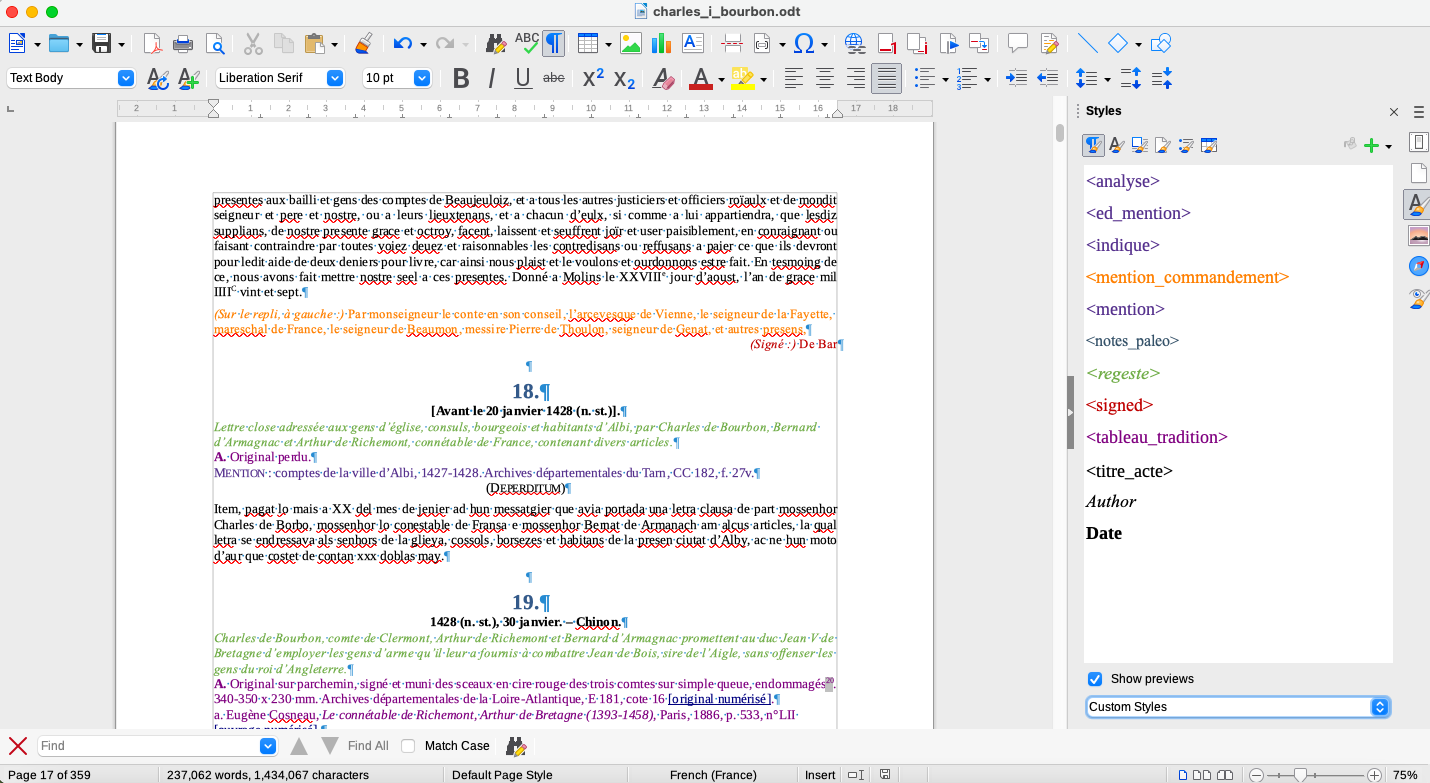
\includegraphics[scale=0.3]{img/deperditum_numerote.png}
    \caption{Deperditum numéroté daté d'avant le 20 janvier 1428.}
    \label{fig:dep_num}
\end{figure}

\par Les deperdita sont les actes pour lesquels le stylage est le plus bref et comporte des variations. À l'instar des autres, les éléments de date et d'analyse sont stylés, le tableau de la tradition également, même s'il est très sommaire : il comporte seulement l'indication que l'original est perdu. La mention du deperditum à la suite du tableau de la tradition a cependant nécessité la création d'un style dédié. Le contenu de cette mention est parfois présent, même si ce n'est pas toujours le cas, ce qui peut impliquer des notes. 
\newline 

\par Une autre variation est attribuable aux différents choix d'édition. En effet, les actes transcrits par Jean-Damien Généro, ceux de Charles I\up{er} et d'Agnès de Bourgogne, sont numérotés, ce qui a impliqué la création d'un style titre structurant pour les numéros. Ces étapes ont nécessité de penser des regex plus ciblées et adaptées aux différents corpus. C’est le cas pour les dates dans le corpus de Charles I\textsuperscript{er}. En effet, quelques actes de ce corpus ne sont pas datés de manière précise et obligent à recourir à des adverbes de temps (avant, après et entre). Là où il s'est avéré relativement simples pour les autres corpus, le stylage des analyses des actes de Charles I\textsuperscript{er} a nécessité une harmonisation de ces dernières (normalisation de leur préambule) afin d'automatiser cette étape. Les analyses des premiers actes reflètent la mise en place progressive de la chancellerie de Charles de Bourbon, qui n'est pas encore duc de Bourbon, mais comte de Clermont, et l'évolution de sa titulature. Les corrections se font plus rares après sa nomination, la titulature de “Charles, duc de Bourbonnais et d’Auvergne” étant définitive. Néanmoins, la plupart des corrections apportées ont permis de pallier un problème normatif. Pour beaucoup d’actes, la mention “de Bourbon” après Charles a été oubliée dans les analyses alors qu’elles étaient présentes dans les actes, elle a donc été rajoutée. 
\newpage 

\par L’autre modification concerne les substantifs placés en début d’analyse, que l'on a souvent transformé en verbes, placés à la suite de la titulature du duc. Par exemple, le “consentement donné par Charles de Bourbon” devient “Charles de Bourbon [...] donne son consentement”. Ensuite, le stylage de ces analyses s’est fait par le recours à de nouvelles regex permettant d’attraper les analyses normalisées. Quelques opérations manuelles ont été réalisées pour les analyses uniques, comme pour les testaments ou les ratifications de contrats de mariage. En tout, trente-deux éditions ont fait l'objet d'une modification manuelle. Les mentions hors teneurs situées à la suite du texte ont bénéficié d'une indentation, étape préalable au stylage de toutes les mentions. 
\newline 

\par Néanmoins, le stylage de certains titres ou sections qui n’ont pas été identifiés par les regex a parfois été réalisé manuellement. Une partie du tableau de la tradition mentionnant les éditions au sein du corpus de Louis II n'a pas pu être stylée automatiquement en raison d'une trop grande proximité stylistique avec les notes paléographiques. En effet, la numérotation des éditions est la même que celle des notes paléographiques (a., b., c., etc). De plus, une partie de ces dernières ont, pour des raisons inconnues, échappé au stylage via des regex, ce qui montre leurs limites d'application à des éditions complexes et non normalisées. Le recours à des logiciels spécialisés dans l’édition critique comme \textit{Classical Text Editor}\footnote{\textit{Classical Text Editor}, en ligne : \url{https://cte.oeaw.ac.at/}} aurait permis un gain de temps sur toutes ces étapes et la génération d'une édition standard. Enfin, certaines parties comme le contenu des actes n’ont pu être stylées et structurées grâce à des regex en raison de leur complexité (intitulations) ou de leur typographie et pourront être manipulées plus facilement après la conversion.

\newpage
\thispagestyle{empty}
\mbox{}
\newpage

\chapter{Conversion des fichiers ODT vers XML/TEI}

\vspace*{\stretch{0.2}} 
\par Le format de document texte OpenDocument (ODT) est un format pour les documents textuels modifiables et un des sous-types de la famille ODF pour certaines catégories de contenu, notamment pour les applications de traitement de texte\footnote{OpenDocument Text Document Format (ODT), Version 1.2, ISO 26300-1:2015, en ligne : \url{https://borntocode.fr/latex-comment-inserer-et-customiser-du-code-source/}.}. La structure et le texte d’un fichier ODT sont tous représentés en XML : les paragraphes et les sections sont facilement reconnaissables, tout comme les en-têtes et les pieds de page, ainsi que les constructions de niveau supérieur grâce à l’utilisation cohérente des styles (par exemple, pour les titres), des tables des matières et des index générés automatiquement, et des modèles structurés. Tout le formatage est représenté dans le document ODT et stocké dans des fichiers XML afin de faciliter la séparation du texte et de la structure sémantique des caractéristiques de mise en page. Les formats de traitement de texte tels que l’ODT stockent de nombreuses informations associées au processus de création et d’examen des documents, y compris les modifications. Toutes ces informations seront interprétées lors de la conversion. L’enjeu est de trouver un convertisseur adapté, dont le résultat reflètera le mieux possible l'édition des actes. Plusieurs convertisseurs ont été testés afin de mesurer leur convenance, celle-ci étant essentiellement basée sur la reproduction de l’organisation des documents. 
\vspace*{\stretch{0.1}} 
\newpage 

\section{Les convertisseurs libres}
\label{II.4.1}

\par D'abord, nous avons testé, par curiosité, deux convertisseurs libres. Premièrement, le niveau de structuration après conversion s’est avéré relativement mauvais. \textit{AnyConv} sépare les actes dans des sections, avec un niveau de titre correspondant à leur numéro\footnote{AnyConv : Convertisseur de ODT en XML, en ligne : \url{https://anyconv.com/fr/convertisseur-de-odt-en-xml/}.}. Hormis cela, tous les éléments sont ensuite encodés dans des balises <para> sans distinction aucune ni précision de la typographie ou des styles. 

\begin{figure}[ht!]
    \centering
    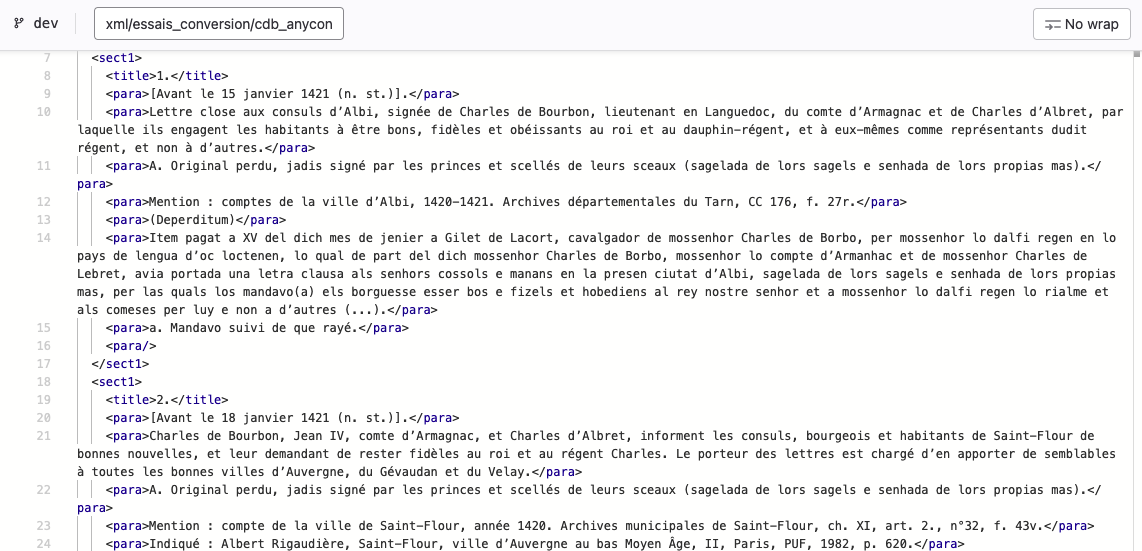
\includegraphics[scale=0.4]{img/any_conv.png}
    \caption{Document XML converti avec \textit{AnyConv}.}
    \label{fig:any_conv}
\end{figure}

\par Le second convertisseur libre testé, \textit{Online ODT converter}, affiche dans un premier temps l’ensemble des styles utilisés, ce qui entrave la lecture\footnote{Online ODT converter, en ligne : \url{https://onlineconvertfree.com/convert/odt/}.}. Ensuite, la structuration est assez chaotique : tout le texte est encodé dans des balises <text>. Malgré la reconnaissance des différents styles ODT et leur affichage comme attributs des balises <text>, il n’y a pas de structuration permettant de refléter la séparation des différents actes. 

\begin{figure}[H]
    \centering
    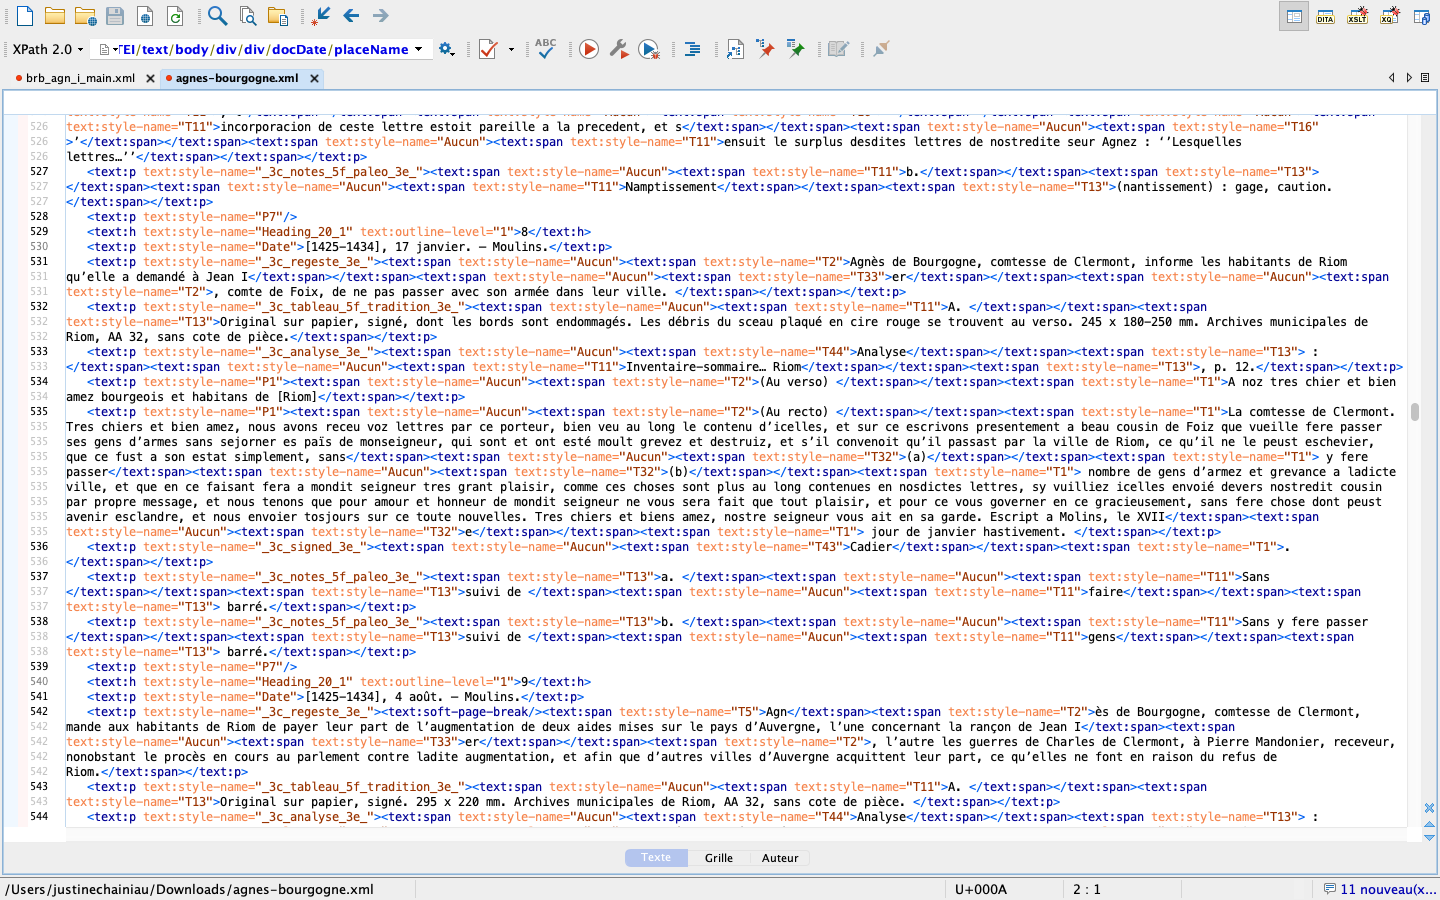
\includegraphics[scale=0.31]{img/onlineconvertfree.png}
    \caption{Document XML converti avec \textit{Online ODT converter}.}
    \label{fig:online_odt_converter}
\end{figure}

\par De plus, l’utilisation de ces convertisseurs pose un problème déontologique avec des développeurs non identifiés et des éditeurs peu fiables. Dans le cadre d’un travail scientifique, il est plus pertinent de favoriser les logiciels développés par la communauté scientifique, généralement plus adaptés aux besoins de cette dernière. D'autre part, ces deux premiers logiciels renvoient des fichiers XML, mais pas au standard TEI.

\newpage 

\section{Essais de conversion avec Pandoc}
\label{II.4.2}

\par Ensuite, nous avons testé une conversion avec \textit{Pandoc} : une bibliothèque Haskell permettant de convertir un format de balisage en un autre, et un outil en ligne de commande qui utilise cette bibliothèque\footnote{Pandoc : a universal document converter, en ligne : \url{https://pandoc.org/}.}. Ce convertisseur a été développé par John MacFarlane, un professeur de philosophie, pour la recherche en Sciences humaines et sociales. Il propose de très nombreuses options de conversion entre différents formats de balisage et de traitement de texte, centrées sur la préservation des éléments structurels d’un document. Nous avons pu tester une conversion de ODT vers XML/TEI, qui s’est montrée plus aboutie. 

\begin{figure}[H]
    \centering
    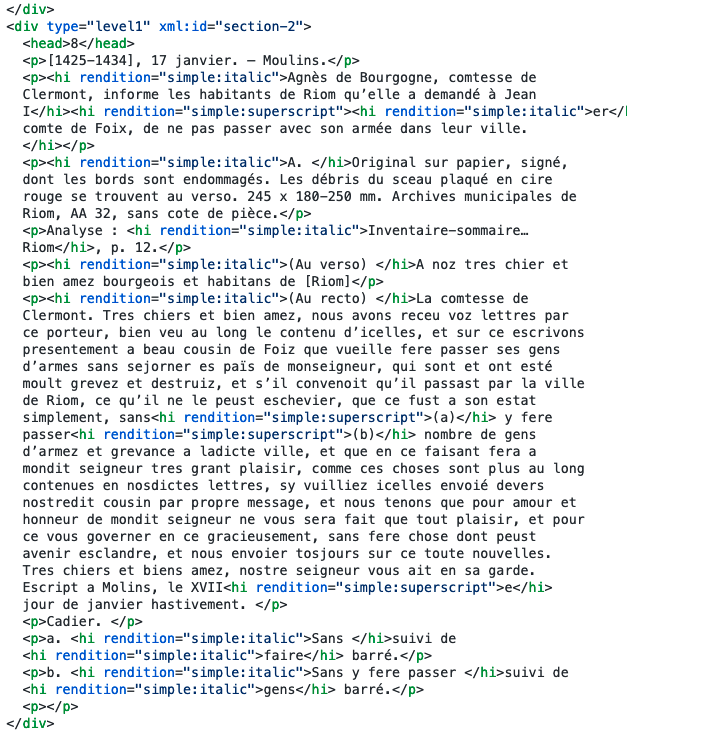
\includegraphics[scale=0.6]{img/pandoc_tei.png}
    \caption{Document XML/TEI converti avec \textit{Pandoc}.}
    \label{fig:pandoc_tei}
\end{figure}

\newpage 

\par En effet, cela a permis la génération d’un TEI Header, à compléter. Le niveau de structuration s’est révélé plus lisible, avec l’inscription de chaque acte dans une balise <div>, avec un niveau de titre pour son numéro (<head>). Tous les éléments sont cette fois-ci encodés dans des balises <p>. Cette conversion a fait ressortir l’organisation du document en différenciant les niveaux de titre (numéro, datation) du corps du texte et les notes de bas de page des notes paléographiques. Toutefois, cette reconnaissance manque de précision dans la mesure où elle ne distingue pas les différentes rubriques de l'édition diplomatique qui ont été stylées avec ODT, que sont l’analyse, le tableau de la tradition et le contenu de l’acte, malgré les différents styles qui leur avaient été appliqués. La différenciation des paragraphes ne se fait qu’à partir des graisses (gras, italique) et non des styles ODT appliqués aux différents éléments. Enfin, une conversion d’un docx vers XML/TEI nous a renvoyé une structuration similaire, mais avec un niveau de précision plus fin et une meilleure reconnaissance de la typographie appliquée aux différents éléments du document. Mais cette conversion n’a pas encore permis l’affichage des différents styles comme attributs. 
\newline 

\par Malgré le niveau de description convenable apporté par \textit{Pandoc} dans le cadre d’une conversion de docx vers XML/TEI, nous avons poursuivi nos tests, afin de voir si la hiérarchisation des éléments et la lisibilité pouvaient être améliorées. 

\newpage 

\section{Choix du convertisseur Teinte}
\label{II.4.3}

\par Enfin, nous avons testé le convertisseur \textit{Odette}, pour textes bureautiques (ODT) en TEI\footnote{Frédéric Glorieux, Odette, convertissez vos textes bureautiques (ODT) en TEI, en ligne : \url{http://obvil.lip6.fr/Odette/}.}. \textit{Odette} a été développée par Frédéric Glorieux, ingénieur de recherche en informatique linguistique et documentaire au Labex OBVIL (Observatoire de la vie littéraire) rattaché à la Sorbonne. Le convertisseur produit des documents structurés en XML/TEI via XSLT, de la qualité la plus élevée possible, à partir d’un traitement de texte\footnote{\cite{glorieuxTraitementTextesOdt2015}.}. La conversion permet par exemple d’éditer des pièces de théâtre classique, avec numérotation des vers, paratexte, index ou glossaire, sans perte d’information. La conversion a permis la génération d’un TEI Header à remplir plus développé. La structuration du document est également mieux respectée : chaque acte est encodé dans une <div>. Le numéro d’acte est encodé dans une balise <head>, les différents éléments sont encodés dans des balises <p> avec comme attributs les différents styles appliqués en amont dans le document ODT, permettant ainsi de refléter une hiérarchie et une structure plus précises. De plus, la date de l’acte est encodée dans une balise <dateline>, ce qui montre que le convertisseur a relevé et reconnu cet élément de datation.
\newline 

\begin{figure}[ht!]
    \centering
    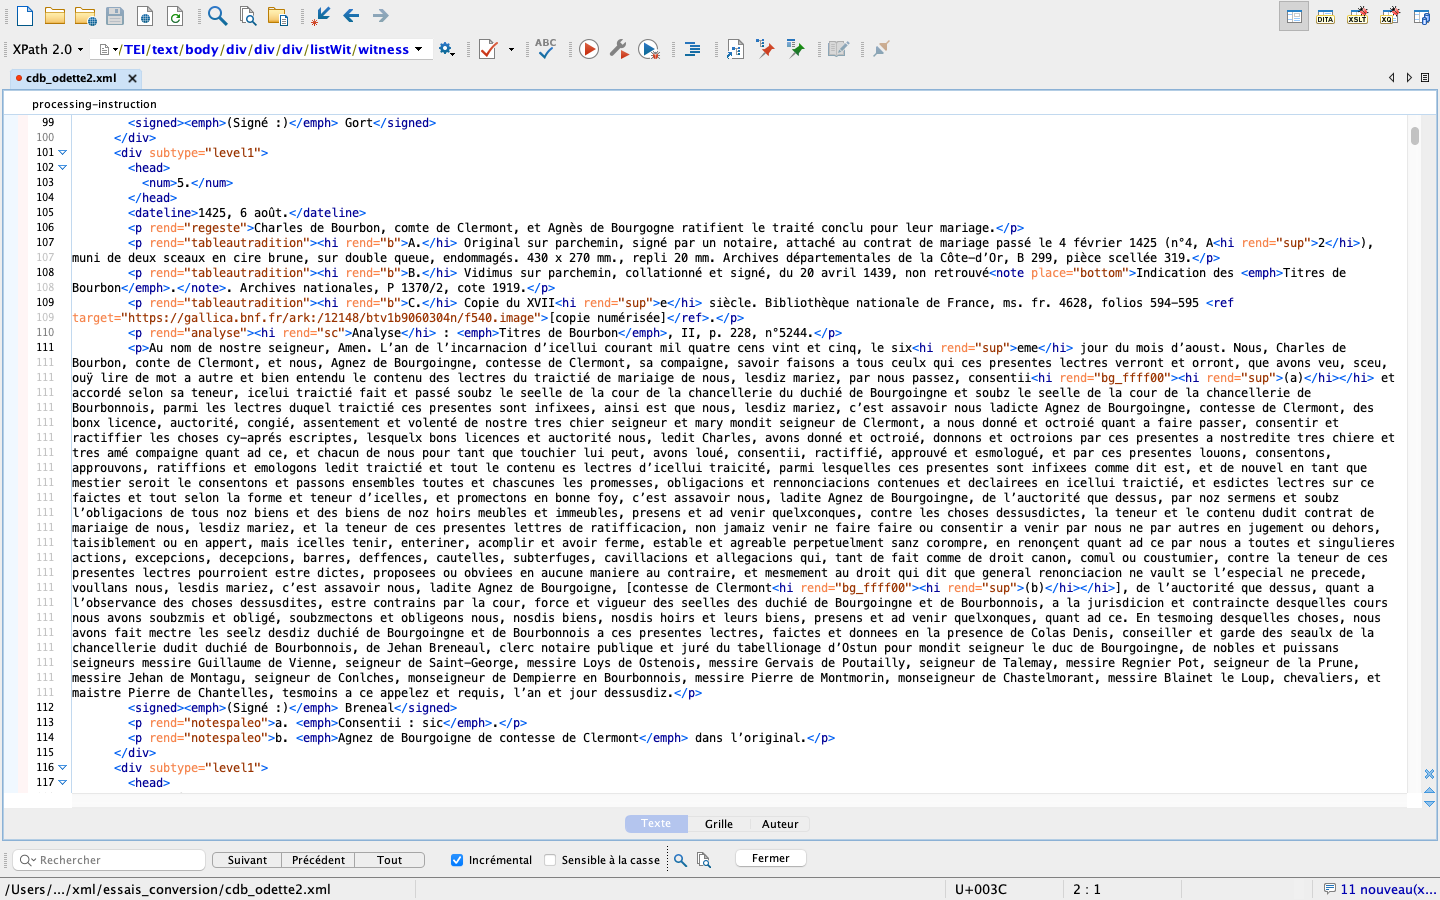
\includegraphics[scale=0.31]{img/odette.png}
    \caption{Document XML converti avec \textit{Odette}.}
    \label{fig:odette}
\end{figure}

\newpage 

\par Néanmoins, avant de trancher sur ce convertisseur, il s’agit d’être certain de sa pérennité et de sa stabilité pour une utilisation ultérieure à d’autres corpus dans le cadre du projet Actes Princiers. Afin de s’en assurer, nous avons contacté le développeur d'\textit{Odette}, F. Glorieux. Il nous a parlé de la refonte d'\textit{Odette} dans \textit{Teinte}, une application en développement continu qui permet la conversion de fichiers TEI, Docx, ePub et txt en TEI, Docx, HTML et txt\footnote{Obtic, Teinte, en ligne : \url{https://obtic.huma-num.fr/teinte/}.}. Il s’agit d’un logiciel libre voué à la pérennité dont l'interface a été financée par le Labex ObTIC (Observatoire des textes, des idées et des corpus) rattaché à la Sorbonne. Nous avons tenté une conversion avec \textit{Teinte}, d’un docx vers XML/TEI. Cette dernière s’est révélée très pertinente. Le document XML/TEI retourné est pourvu d’un TEI Header à remplir. Toutefois, ce dernier reste succinct et sera à repenser dans le cadre d’une édition globale des actes princiers. 

\begin{figure}[ht!]
    \centering
    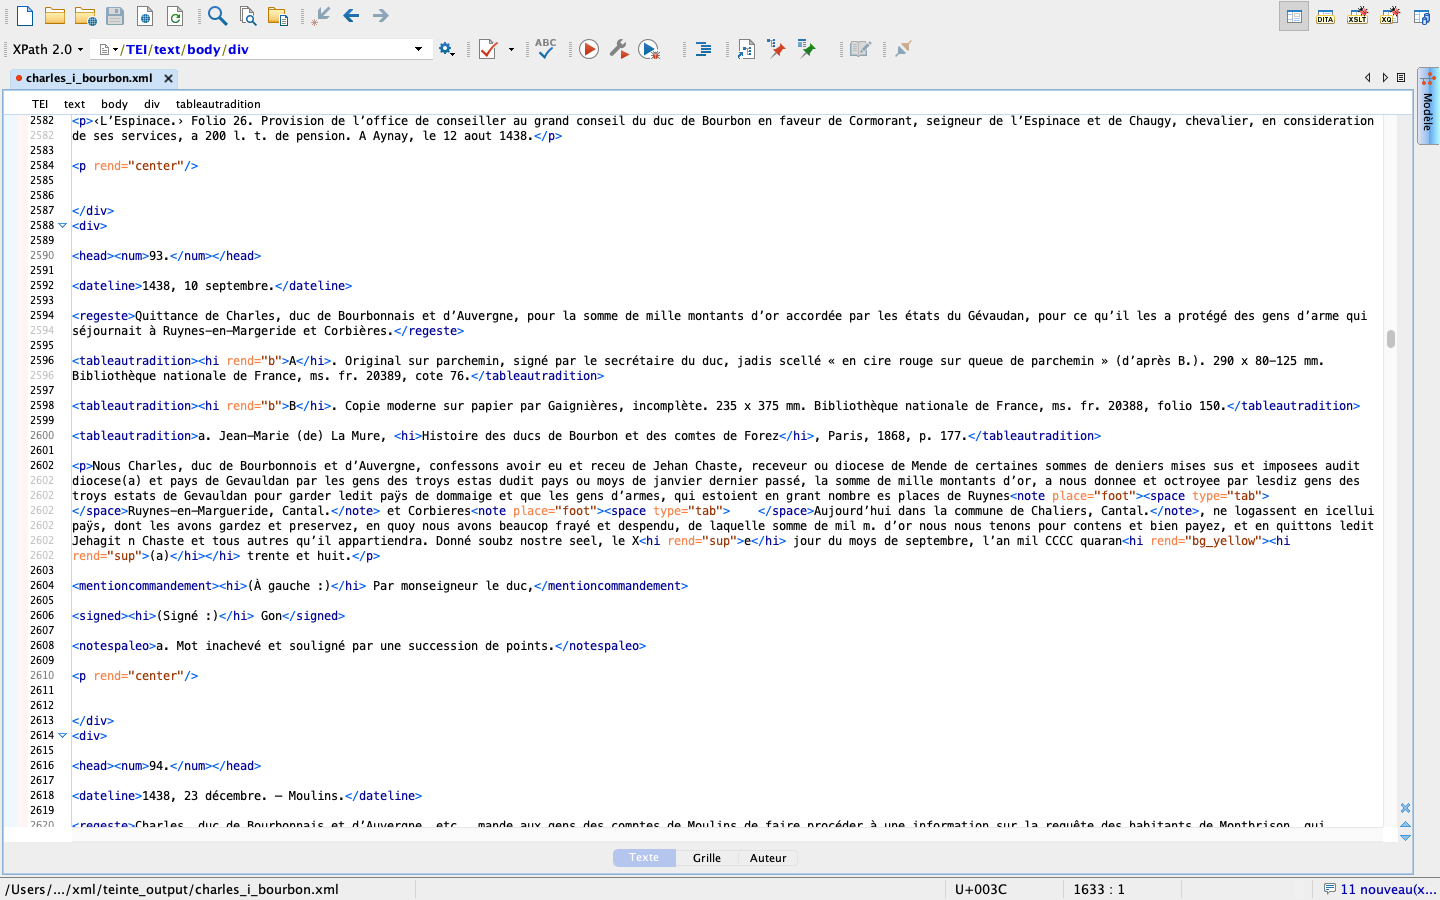
\includegraphics[scale=0.31]{img/teinte.png}
    \caption{Document XML/TEI converti avec \textit{Teinte}.}
    \label{fig:teinte}
\end{figure}

\par Comme nous pouvons le voir ci-dessus, le recours à des styles personnalisés et normalisés par un utilisateur sur ODT permet la transformation de ces derniers en éléments (balise avec son contenu textuel). Cela implique une meilleure hiérarchisation des différents éléments diplomatiques. La compréhension est améliorée via la structuration du document et des différentes parties de l'édition dans des balises appropriées. De plus, \textit{Teinte} est un projet développé pour la recherche en sciences humaines et sociales, voué à se pérenniser. Même si le résultat de la transformation ne renvoie pas des balises XML, ces dernières, ainsi que l'organisation du document pourront être repensés et retravaillés. 

\newpage
\thispagestyle{empty}
\mbox{}
\newpage
    
    \part{La chaîne de traitement des actes princiers}

\chapter[Structuration des XML]{Structuration des XML à partir d'un script Python}

\vspace*{\stretch{1.3}} 
\par La conversion des documents ODT en XML avec \textit{Teinte} renvoie des documents TEI relativement structurés. Néanmoins, les balises ne sont pas conformes au format TEI. De plus, la structuration du document peut être encore améliorée, via la création d'attributs (caractéristiques d'une balise) par exemple. Le langage de programmation Python va permettre de lire les fichiers et d'intervenir dessus afin de parfaire l'organisation des actes. Python est un langage de programmation développé dans les années 1990 par le développeur Guido van Rossum. Il fournit une approche simple et efficace de la programmation orientée objet\footnote{La programmation orientée objet, ou programmation par objet, est une manière d'approcher la programmation via l'interaction de briques logicielles appelées objets. Les objets sont des structures de données avec le comportement associé, manipulés dans un programme. In : \cite{ProgrammationOrienteeObjet2021}.}, ce qui en fait un langage idéal pour les scripts et le développement d’applications dans de nombreux domaines\footnote{\og Le tutoriel Python \fg, in : \cite{ContenuDocumentationPython}.}.


\vspace*{\stretch{0.7}} 

\newpage 

\section[Extraction / Injection des données]{Extraction de données à partir des fichiers CSV et injections dans le XML
}
\label{III.5.1}

\par Une partie des données relatives aux actes de Charles I\up{er}, d’Agnès de Bourgogne et d’Anne Dauphine sont présentes dans un document CSV. Le format CSV, dont les valeurs sont séparées par des virgules, est le format le plus commun dans l'importation et l'exportation de feuilles de calculs et de bases de données\footnote{\og Lecture et écriture de fichiers CSV \fg, in : \cite{ContenuDocumentationPython}.}. Les CSV répertorient pour chaque duc et duchesse des informations essentielles sur les actes comme leur numéro, l'institution de conservation, le fond dont ils sont issus (identifiants), leur état, leur type diplomatique, l’année et la date de rédaction, les signataires, le lieu, les mentions de commandement, la langue de l'acte, et la présence ou non d’un sceau. 
\newline

\begin{figure}[ht]
    \centering
    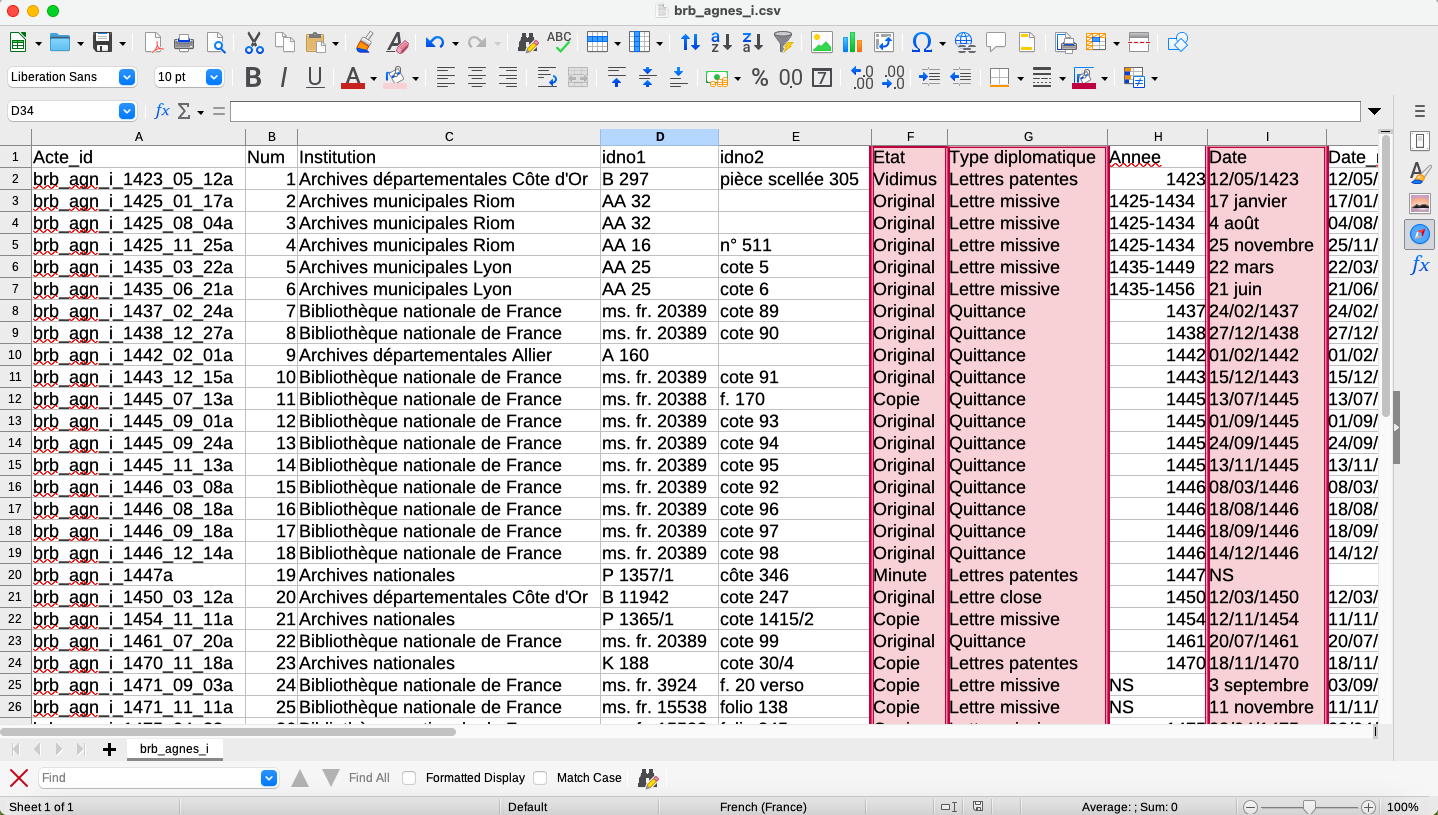
\includegraphics[scale=0.31]{img/csv_ad.png}
    \caption{CSV actes d'Agnès de Bourgogne.}
    \label{fig:csv}
\end{figure}

\par L’enjeu est d’extraire une partie des données des CSV : la date, l'état et le type diplomatique de chaque acte (valeurs surlignées en rose dans le tableur ci-dessus) afin de les ajouter comme attributs de la balise <div> du fichier XML créé pour chaque corpus. La date permettra également la création d'un attribut prenant la valeur d'un identifiant unique (@xml:id), pour chaque acte. Afin d'illustrer au mieux les modifications réalisées via Python, les figures qui suivent (figures 5.2 à 6.2) montrent les états successifs de l'acte daté du vingt-quatre février 1437 dans la chaîne de traitement des actes princiers.
\newpage 

\par Pour extraire les données en question, un script Python a été écrit\footnote{GitLab (py/add\_csv\_infos.py).}. 
\newline 
\par D'abord, une première fonction assure la lecture des fichiers XML à l'aide de la librairie \textit{BeautifulSoup}. Cette dernière permet l’extraction de données de fichiers HTML et XML. Afin de pouvoir l’utiliser correctement avec des fichiers XML, il est nécessaire d'importer le module \og bs4 \fg \space et d'installer le parseur \og lxml \fg \space conçu à cet effet. \textit{BeautifulSoup} fournit des moyens de navigation, de recherche et de modification de l’arbre XML. 
\newline 
\par Ensuite, une deuxième fonction constitue une liste avec les données du CSV qui seront transformées en attributs de la balise <div>. Elle nécessite d'importer le module \og csv \fg, qui permet de lire et d'écrire des données au format tabulaire CSV via les objets \og reader \fg \space et \og writer \fg. La fonction applique aux différents formats de dates un format standard afin de les agréger à un identifiant unique : xmlid. Deux modules sont importés pour assurer ces opérations : le module \og datetime \fg, qui fournit des classes pour manipuler les dates qui est complété par le module \og locale \fg \space qui prend en compte les spécificités de datation locales. La fonction comporte une première boucle qui itère sur chaque ligne du CSV. Si la valeur de la date est égale à \og Dep. \fg \space (deperditum), alors la date est manquante et un identifiant est créé. Si la date n’est pas \og Dep.\fg, une série de formats de date possibles est définie et stockée dans une liste. La fonction comprend une seconde boucle qui itère sur chaque format de date, les analyse, et en assure la conversion dans un format standard (YYYYMMDD). Elle permet également la création d'un identifiant unique pour chaque acte, à partir de cette date. La fonction retourne un dictionnaire composé des données extraites du CSV : date standard, état et type diplomatique, en préparation de leur injection aux fichiers XML. 
\newline 
\par Enfin, une troisième fonction injecte les données dans le XML. Après ouverture et lecture du fichier XML, elle itère sur toutes les balises <div> du <body> et leur ajoute les données extraites et modifiées comme attributs. L'attribut \og n \fg \space prend comme valeur la date au format standard, l'attribut \og xml:id \fg, l'identifiant unique créé à partir de cette date, l'attribut \og type \fg, l'état et l'attribut \og subtype \fg, le type diplomatique. Quelques opérations de mise en forme des documents ont été éfectuées, comme la suppression des lignes vides dans le nouveau document XML, via des expressions régulières, ce qui a nécessité l'importation du module \og re\fg. Les apostrophes odt sont également remplacées par des apostrophes standard et les balises <dateline> par des balises <head>. Les fichiers de sortie comportent les modifications réalisées par les trois fonctions. 
\newpage 

\begin{figure}[ht]
    \centering
    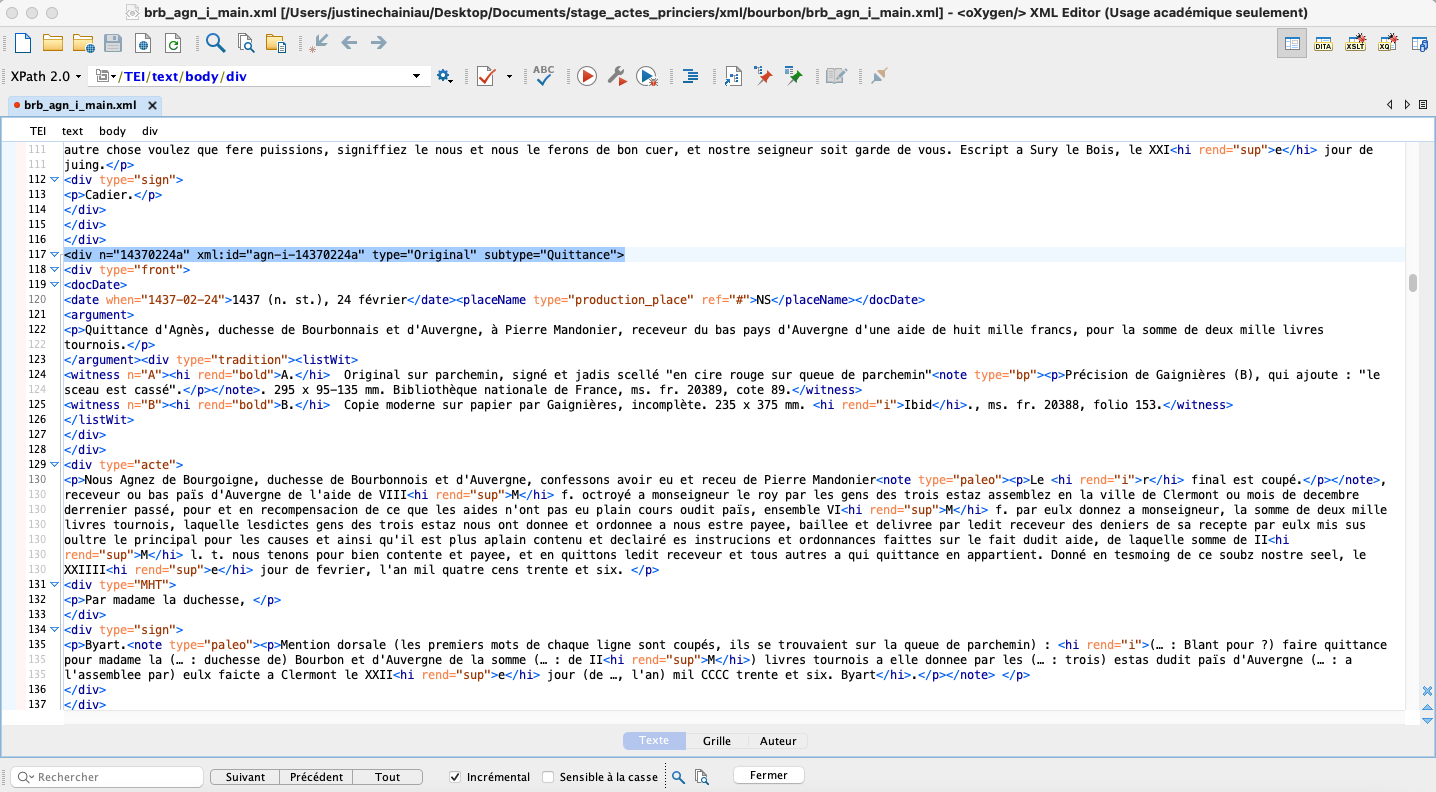
\includegraphics[scale=0.29]{img/injection.png}
    \caption{XML après injection des données avec Python.}
    \label{fig:injection}
\end{figure}

\par Les fonctions créées ont permis l'extraction de données de fichiers CSV et l'ajout de ces mêmes données dans du XML pour les actes d'Anne Dauphine, de Charles I\up{er} et d'Agnès de Bourgogne. Toutefois, les actes du corpus de Louis II ne sont pas répertoriés dans un CSV. Nous avons donc inversé la procédure afin d'en créer un.
\newline 

\par La fonction xml\_to\_csv créé un fichier CSV à partir de données extraites du fichier XML répertoriant les actes de Louis II\footnote{GitLab (py/div\_attributes.py).}. Une boucle itère sur chaque balise <div> et remplit, à partir d'information récupérées dans le XML, une liste. La fonction récupère le contenu de la balise <dateline>, qu'elle sépare en deux parties à partir d'une boucle. Si l'élément séparateur \og -\fg \space est présent dans le texte de la variable date, alors ce texte est divisé en deux parties qui forment deux items, afin de séparer la date de temps de la date de lieu. Sinon, le lieu n'est pas précisé et la mention \og NS\fg\footnote{NS : Non signalée.} \space est inscrite. La chaîne de caractère \og Louis II\fg \space est définie par défaut comme avant-dernier item de la liste, comme valeur de la colonne \og prince\fg. Pour la colonne \og signataire \fg, si la balise <signed> est présente dans les <div>, alors on complète la liste avec le contenu textuel de la balise <signed>, en omettant les diverses mentions \og (signé:)\fg. Autrement, la mention \og NS\fg \space lui est ajoutée. La mention \og fr\fg \space est répertoriée par défaut comme dernier item de la liste, comme valeur de la colonne \og langue\fg. En effet, seuls trois actes de Louis II sont en latin et ont été repérés préalablement : la colonne langue prend alors la valeur \og lat \fg \space pour les actes concernés\footnote{La Mure III, p.132 (10 juin 1370) - AD Allier, 1 G 3, fol. 1-6 (6 décembre 1386) \newline AN, P 1356\up{2}, c. 280 (18 septembre 1399).}. 
\newpage 

\par Ensuite, le fichier CSV est ouvert via la fonction \og open() \fg \space de Python, et les lignes sont remplies à partir des données stockées dans la liste. La ligne d'en-tête du fichier CSV est écrite à partir de la spécification du nom des colonnes : \og Date\fg, \og Lieu\fg, \og Prince\fg, \og Signataire\fg, \og Langue\fg, \og État\fg, \og Type diplomatique\fg. Néanmoins, ces deux dernières colonnes n'ont pu être complétées automatiquement, mais manuellement via le relevé de l'état de chaque acte et de son type diplomatique à partir du document ODT.
\newline 

\par La programmation en Python permet d'automatiser la manipulation des données, et ainsi de gagner du temps dans la chaîne de traitement. Toutefois, le processus se fonde sur les premiers corpus, qui disposent de fichiers CSV répertoriant les actes. En effet, la chaîne de traitement des actes princiers, telle qu'elle a été pensée par les ingénieurs du projet, nécessite qu'un certain nombre d'informations sur les actes soient présentes dans des fichiers CSV. Il faudra donc que les nouveaux corpus ajoutés au projet aient un CSV associé. Autrement, Python permet leur création via des fonctions, mais toute la procédure ne peut pas être automatisée, et toutes les colonnes remplies à partir de l'extraction de données. Des notions de diplomatique sont nécessaires afin de repérer, via la lecture de tous les actes, les états et les types diplomatiques, ce qui prend un certain temps, notamment dans le cas de corpus volumineux, comme ceux de Louis II et de Charles I\up{er}. Le projet \og Actes princiers \fg \space pourrait donc conseiller aux chercheurs qui élaborent des éditions diplomatiques de dresser en parallèle un tableur avec les différentes métadonnées. Les corpus disposent désormais tous d'un fichier CSV rempli, et les fichiers XML d'une balise <div> pourvue d'attributs qui contribuent à affiner l'organisation du document. Chaque acte est contenu dans une division (<div>) du document XML et identifié en tant que tel. Comme l'ensemble des balises n'est pas normalisé, les fonctions vont permettre de restructurer de manière automatique les documents XML.
\newpage 

\section[Restructuration des documents XML]{Restructuration des documents XML issus de la conversion}
\label{III.5.2}

\par Les documents XML obtenus en sortie, après intervention via un script Python, comportent désormais une balise <div> structurée. Toutefois, c'est l'ensemble du document qui nécessite d'être hiérarchisé. Il s'agit donc en utilisant Python de restructurer les documents selon le plan d'encodage ci-après, notamment en remplaçant les balises obtenues après conversion avec \textit{Teinte} en balises TEI afin d'obtenir un document XML valide. Comme l'indique le schéma ci-après, chaque acte doit être encodé dans une balise <div> comportant cinq autres balises <div>, qui représentent des subdivisions du corps du document\footnote{TEI Guidelines, <div>, en ligne : \url{https://tei-c.org/release/doc/tei-p5-doc/en/html/ref-div.html}.}. 
\newline 
\par La première d'entre elles comporte les éléments de datation et d'analyse. Les dates de temps et de lieu sont encodées dans deux balises distinctes. Le tableau de la tradition est ensuite structuré en une liste de témoins (<listWit>). Chaque témoin est encodé dans une balise dans laquelle sont imbriquées des balises pour le texte, l'institution de conservation et les identifiants (fonds et cote). Ensuite, une troisième <div> contient la teneur de l'acte dans une balise <p>, qui marque le début d'un paragraphe en prose\footnote{TEI Guidelines, <p>, en ligne : \url{https://tei-c.org/release/doc/tei-p5-doc/en/html/ref-p.html}.}. Si l'acte comporte un titre, il est encodé dans une balise <head>, qui marque l'en-tête (<head>Texte établi d'après A.</head>, <head>(Deperditum)</head>)\footnote{TEI Guidelines, <head>, en ligne : \url{https://tei-c.org/release/doc/tei-p5-doc/en/html/ref-head.html}.}. Pour finir, deux dernières balises <div> contiennent les mentions hors teneurs et les signataires dans des balises <p>. Ces opérations sont consignées dans des fichiers Python individuels pour chaque corpus : regex\_anne\_dauphine\footnote{GitLab (py/regex\_anne\_dauphine.ipynb).}, regex\_brb\_agnes\footnote{GitLab (py/regex\_brb\_agnes.ipynb).}, regex\_charles\footnote{Gitlab (py/regex\_charles\_i.ipynb).}, regex\_louis\footnote{GitLab (py/regex\_louis\_ii.ipynb).}. Il n'a pas été possible de traiter les quatre corpus à partir d'un seul script, car les documents ODT initiaux ne sont pas exactement structurés de la même manière. 

\begin{figure}[H]
    \centering
    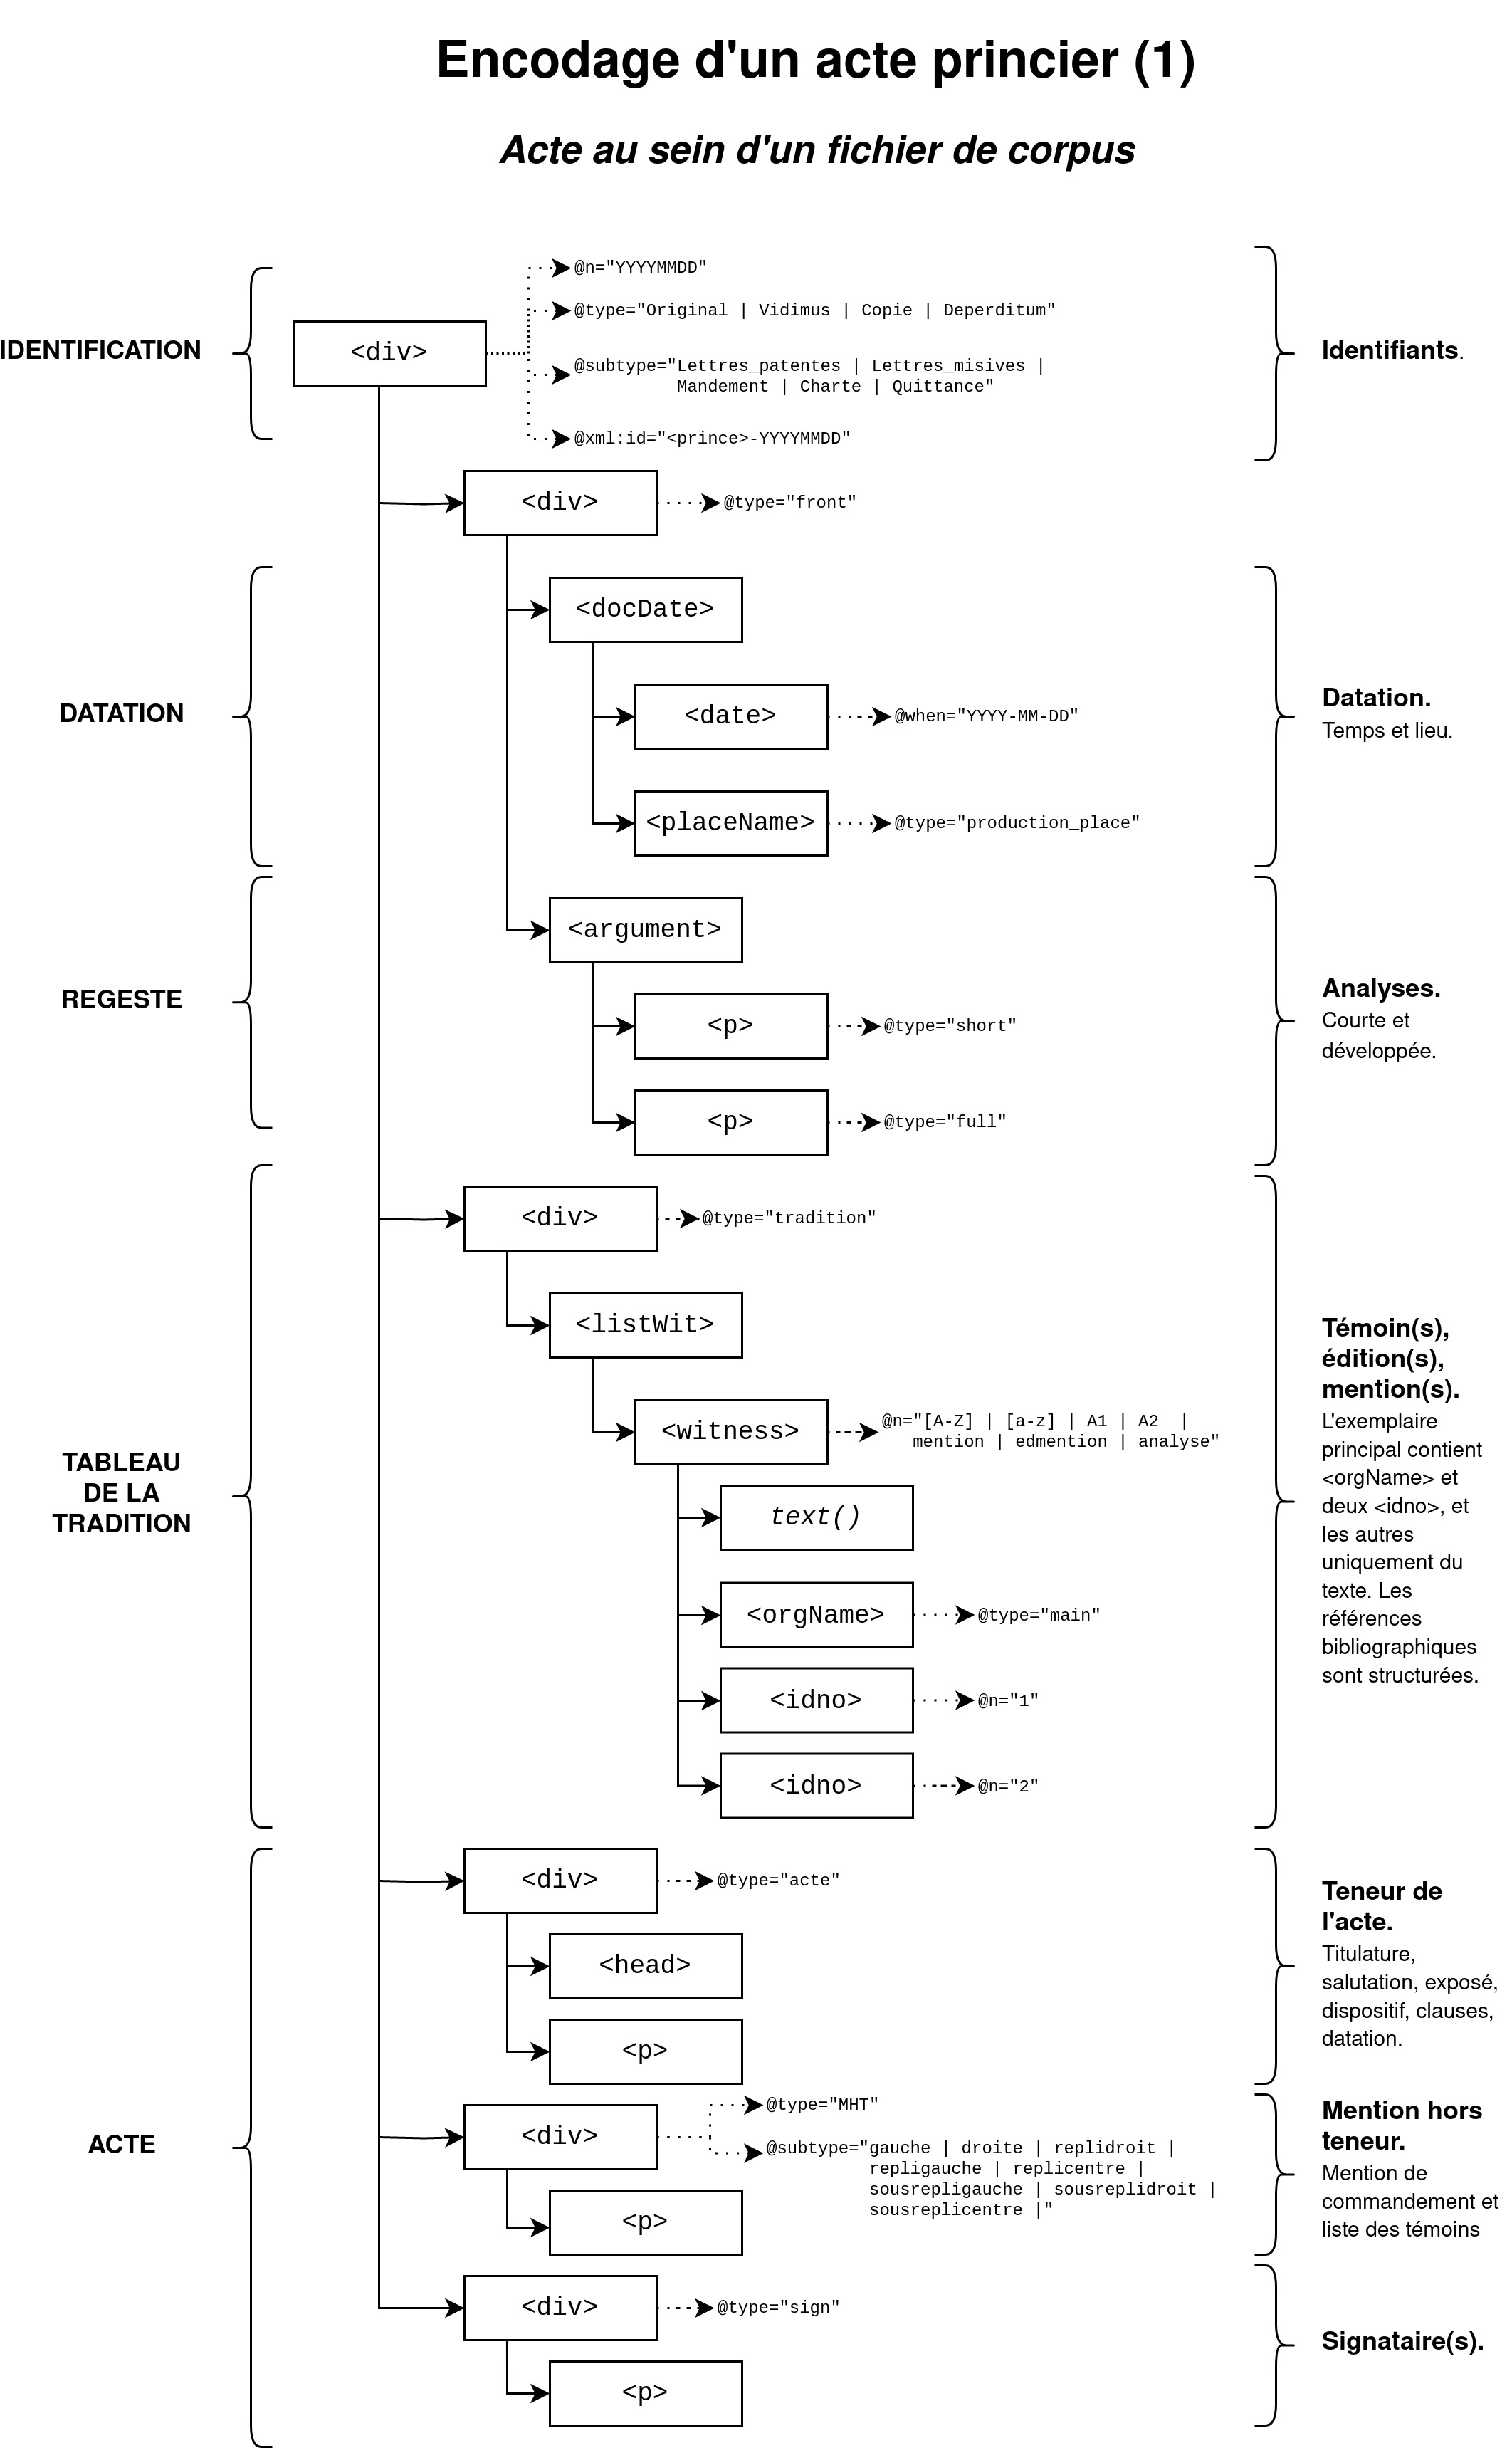
\includegraphics[scale=0.18]{img/encodage_actes_corpus.jpg}
    \caption{Schéma d'encodage des actes en XML. Source : Jean-Damien Généro.}
    \label{fig:encodage}
\end{figure}
\newpage 

\par D'abord, le script réalise des traitements automatiques via des regex pour améliorer la mise en forme des documents. Grâce à la fonction \og re.sub \fg, le code supprime un certain nombre d'éléments inutiles (balises inutiles, lignes vides) et substitue certaines balises afin d'obtenir une structuration plus fine. Ces opérations de substitution permettent l'insertion des principales <div> et éléments structurants comme <docDate>, spécifique pour la datation de documents\footnote{TEI Guidelines, <docDate>, en ligne : \url{https://tei-c.org/release/doc/tei-p5-doc/en/html/ref-docDate.html}.}, <argument>, cette dernière contenant une liste formelle ou une description en prose des sujets abordés dans une subdivision\footnote{TEI Guidelines, <argument>, en ligne : \url{https://tei-c.org/release/doc/tei-p5-doc/en/html/ref-argument.html}.} et <listWit>, qui énumère tous les témoins mentionnés par un appareil critique, éventuellement regroupés hiérarchiquement\footnote{TEI Guidelines, <listWit>, en ligne : \url{https://tei-c.org/release/doc/tei-p5-doc/en/html/ref-listWit.html}.}. Les illustrations à la page suivante donnent un aperçu des fichiers avant et après les interventions. Les premières balises structurantes sont ajoutées : <div type='front'> et <docDate> avec ses balises enfants. La balise <regeste> (qui peut être suvi d'une balise <hi>, marquant un mot ou une phrase comme graphiquement distinct du texte environnant\footnote{TEI Guidelines, <hi>, en ligne : \url{https://tei-c.org/release/doc/tei-p5-doc/en/html/ref-hi.html}.}) est substituée par la balise <argument> suivie d'une balise <p>. La fonction \og re.sub \fg permet la fermeture de certaines balises comme <p> et <argument> et d'intégrer les balises ouvrantes suivantes : <div type='tradition'> et <listWit>. Cette opération est répétée afin de fermer la balise </listWit> et d'ajouter les suivantes : </div>, </div>, <div type="acte"> et <p>. Les cas particuliers des actes commençant par un titre ou comportant la mention \textit{deperditum} sont réglés par des regex. Puis, la balise <div type="acte"> est fermée, ainsi que celle du dernier acte, dont le traitement n'est pas automatique. Le <tableautradition> est suppléé par la balise <witness> contenant la description précise d’un seul témoin\footnote{TEI Guidelines, <witness>, en ligne : \url{https://tei-c.org/release/doc/tei-p5-doc/en/html/ref-witness.html}.}, avec ses attributs et suivi du n° d'exemplaire. Les spécifications <analyse>, <edmention> et <mention> sont toutes remplacées par la balise <witness>, dont la balise fermante est ajoutée. Les dernières balises <mentioncommandement> et <signed> sont changées en balises <div> disposant respectivement d'attributs \og MHT \fg \space et \og sign \fg. 
\newpage

\begin{figure}[H]
    \centering
    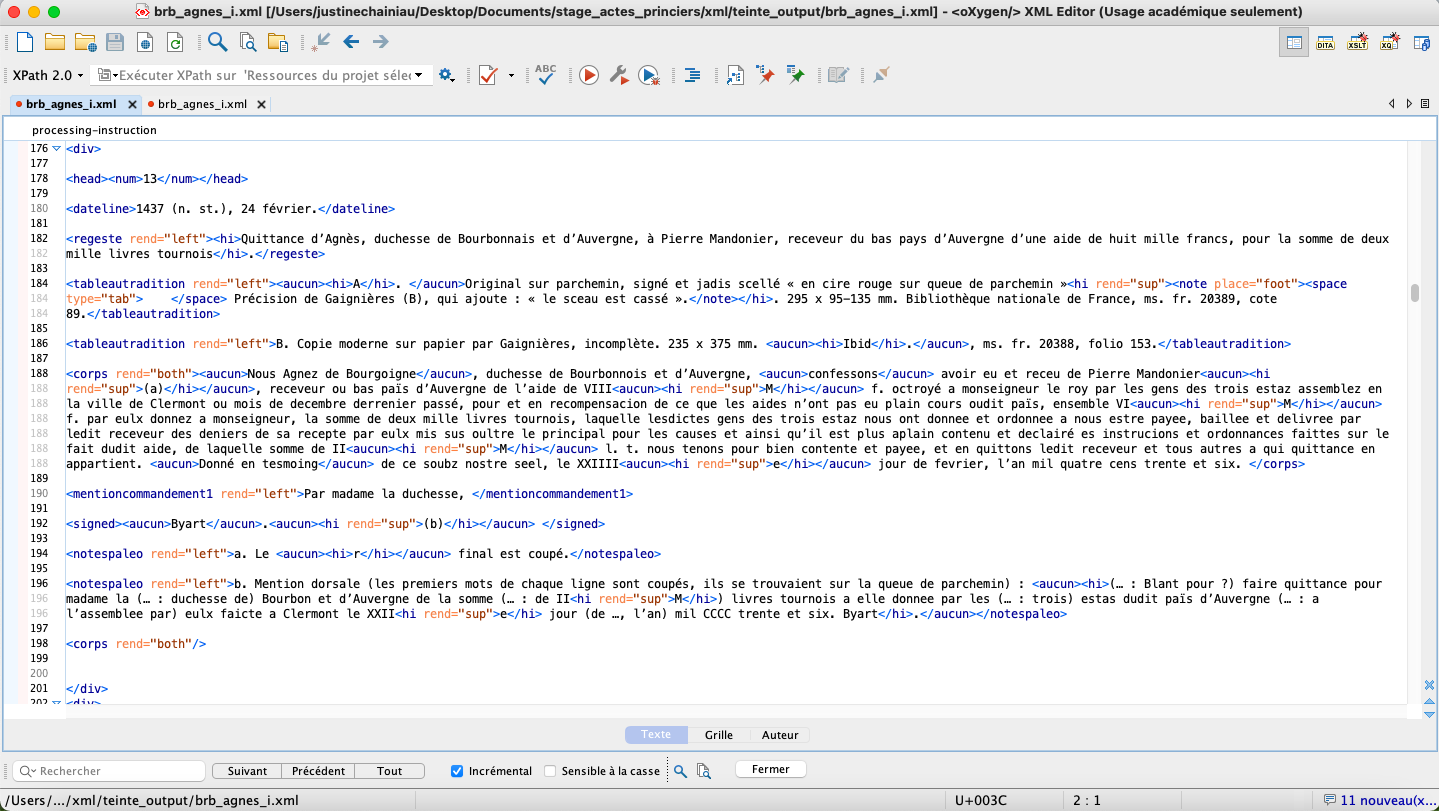
\includegraphics[scale=0.3]{img/teinte_agnes.png}
    \caption{Encodage de l'acte daté du 24 février 1437 avant intervention.}
    \label{fig:encodage_avant}
\end{figure}

\begin{figure}[H]
    \centering
    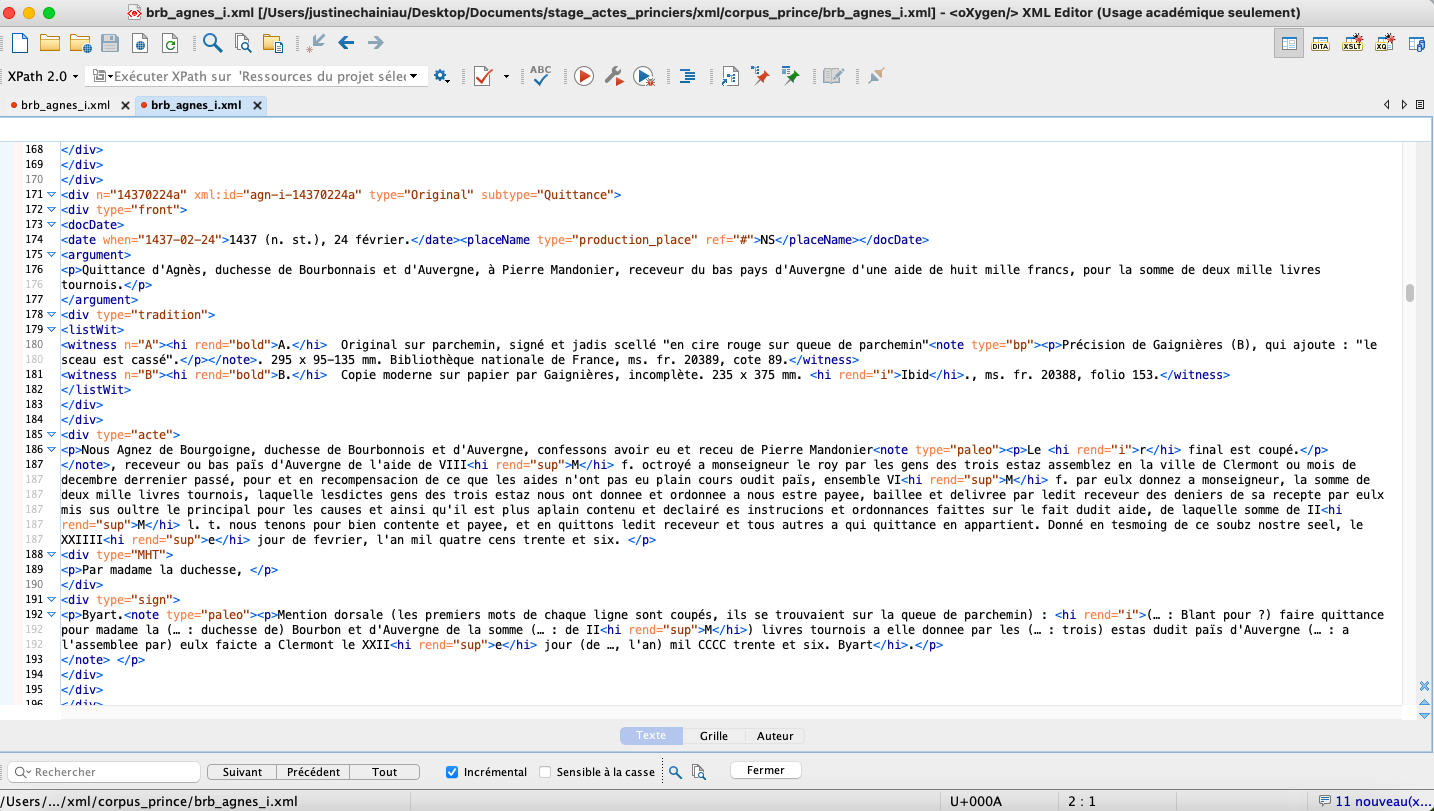
\includegraphics[scale=0.3]{img/restruct_agnes.png}
    \caption{Encodage de l'acte daté du 24 février 1437 après intervention.}
    \label{fig:encodage_après}
\end{figure}
\newpage 

\par Ensuite, le script réalise des traitements semi-automatiques. En raison des disparités entre les quatre corpus, toutes les opérations ne peuvent pas être réalisées de manière automatique. De plus, les regex de l'étape précédente n'ont pas toujours fonctionné. En effet, la chaîne de traitement bute sur des erreurs de mise en forme des éditeurs. L'option de validation d'Oxygen nous a permis de repérer les problèmes d'encodage et de les corriger un à un dans le script via une regex dédiée. Ces irrégularités sont pour une grande partie liées à la balise <hi> qui est parfois présente en trop ou manquante. De plus, les mentions \og (Signé :) \fg \space comportent des fautes d'encodage et n'ont, par conséquent, pas toujours été supprimées par le script. Les erreurs spécifiques à chaque corpus sont traitées individuellement. Toutes les corrections sont stockées dans un dictionnaire qui se substituera aux valeurs précédentes. Les dernières erreurs concernent la mise en forme des notes de bas de page et des notes paléographiques. Le nombre d'appels de note diffère du nombre de notes. Cela est généralement dû aux manquements dans le stylage effectué précédemment, ou à leur présence en double. Après quelques corrections de mise en forme : traitement des espaces insécables, des guillemets, des balises <hi> sans attributs, le fichier est écrit dans un document. Le parseur lxml repère les fautes de syntaxe et traite les caractères non valides. Les éléments HTML, s'il y en a, sont retirés et les octets XML sont décodés en une chaîne de caractères afin d'inscrire le contenu XML dans un fichier.
\newline 

\par Enfin, en fonction des erreurs relevées, des corrections sont effectuées avec lxml. L'objectif principal est la structuration des dates en un bloc. Pour cela, il s'agit d'ajouter à la nouvelle balise <date> un attribut \og when \fg \space avec la date au format standard YYYYMMDD, ou YYYYMM ou YYYY. Puis, les notes paléographiques sont alignées sur leurs appels de note. La dernière correction concerne les attributs \og xml:id \fg \space et \og n \fg. En effet, lorsque deux actes sont datés du même jour, ils ont le même identifiant, or ces derniers doivent être uniques dans un document XML.
\newline 

\par La suppression et la substitution de balises via une fonction Python a permis de structurer très finement les documents avec des balises XML imbriquées et dotées d'attributs. Toutefois, certaines opérations se sont montrées plus complexes, comme la hiérarchisation du tableau de la tradition, qui n'est pas aussi fine que sur le schéma d'encodage établi en amont\footnote{Figure 5.3 – Schéma d’encodage des actes en XML.}. En effet, la balise <witness> ne comporte pas les balises <text>, <orgName> et <idno>. Même si le document obtenu en sortie ne respecte pas exactement le schéma théorique, la plupart des balises ont été transformées. Les fichiers XML bénéficient désormais d'une structure robuste permettant leur division en fichiers XML individuels pour chaque acte.
\newpage 


\section[Séparation des fichiers]{Séparation des fichiers XML de corpus en fichiers XML d’actes}
\label{III.5.3}

\par L'objectif est de transformer le fichier XML contenant l'ensemble des actes d'un prince obtenu après interventions en autant de fichiers XML qu'il y a d'actes. Une fonction Python : split\_corpus\footnote{GitLab (py/split\_corpus.ipynb).} est utilisée pour réaliser cette opération. Cette fois-ci, une seule fonction est adaptable pour les quatre corpus, dans la mesure où ils ont été normalisés en amont. La première étape est la création d'un fichier XML par acte. Cela passe par la récupération des <div> des actes en itérant sur chaque balise. Les données sont alors stockées dans une liste, qui, couplée au canevas TEI suivant, permet la constitution du fichier.
\newline 

\textbf{CANEVAS TEI} \newline 
<TEI xmlns="http://www.tei-c.org/ns/1.0"> \newline 
<teiHeader> \newline 
<fileDesc> \newline 
<titleStmt> \newline 
<title level="s">Actes princiers</title> \newline 
<title level="m">+++TITLE+++</title> \newline 
<title level="a"></title> \newline 
<respStmt> \newline 
<resp>transcribed by</resp> \newline 
<name>+++TRANSCRIPTEUR+++</name> \newline 
</respStmt> \newline 
</titleStmt> \newline 
<editionStmt> \newline 
<edition>Acte édité dans le cadre du programme Actes princiers.</edition> \newline 
<respStmt> \newline 
<resp>direction scientifique</resp> \newline 
<name>Olivier Mattéoni</name> \newline 
</respStmt> \newline 
<respStmt> \newline 
<resp>direction technique</resp> \newline 
<name>Jean-Damien Généro</name> \newline 
</respStmt> \newline 
<respStmt> \newline 
<resp>direction technique</resp> \newline 
<name>Nicolas Perreaux</name> \newline 
</respStmt> \newline 
<respStmt> \newline 
<resp>stagiaire de l'École nationale des chartes</resp> \newline 
<name>Justine Chainiau</name> \newline 
</respStmt> \newline 
</editionStmt> \newline 
<publicationStmt> \newline 
<publisher>Laboratoire de Médiévistique occidentale de Paris (UMR 8589), Centre de recherches historiques (UMR 8558)</publisher> \newline 
<authority>Olivier Mattéoni</authority> \newline 
<date when="2023">2023</date> \newline 
<availability><licence source="https://github.com/etalab/licence-ouverte/blob/master/open-licence.md">Distributed under an Open License 2.0</licence></availability> \newline 
</publicationStmt> \newline 
<sourceDesc> \newline 
<msDesc> \newline 
<msIdentifier> \newline 
<repository></repository> \newline 
</msIdentifier> \newline 
<msContents> \newline 
<msItem> \newline 
<docDate></docDate> \newline 
</msItem> \newline 
</msContents> \newline 
</msDesc> \newline 
<listPerson> \newline 
<listPerson type="prince"/> \newline 
<listPerson type="signatory"/> \newline 
</listPerson> \newline 
</sourceDesc> \newline 
</fileDesc> \newline 
<profileDesc> \newline 
<abstract> 
<p></p> 
</abstract> \newline 
</profileDesc> \newline 
</teiHeader> \newline 
<text> \newline 
<body> \newline 
</body> \newline 
</text>
</TEI> \newline 

\par La fonction complète le TEI Header ci-dessus avec une partie des données présente dans le CSV. Le nom du prince à l'origine de l'acte est ajouté à la balise <listPerson type="prince">, ceux des signataires dans la balise <listPerson type="signatory">. L'institution de conservation, le fonds et la cote sont également extraits des colonnes du CSV. Les éléments HTML sont encore une fois retirés, et les octets XML décodés en une chaîne de caractère afin d'inscrire le contenu XML dans un fichier. 
\newline 

\par L'activation des fonctions passe par la création d'un dictionnaire contenant en clef l'identifiant de la maison et celui du prince, et en valeur une liste avec : le chemin vers le fichier XML du prince depuis le dossier /py, le nom du CSV du prince, le nom du dossier où seront enregistrés les XML des actes, le titre du corpus et le nom du transcripteur. La fonction est activée via une itération sur le dictionnaire et permet la transformation des fichiers. Le fichier ci-après montre le résultat obtenu après division du fichier contenant tous les actes du corpus. 
\newline 

\begin{figure}[H]
    \centering
    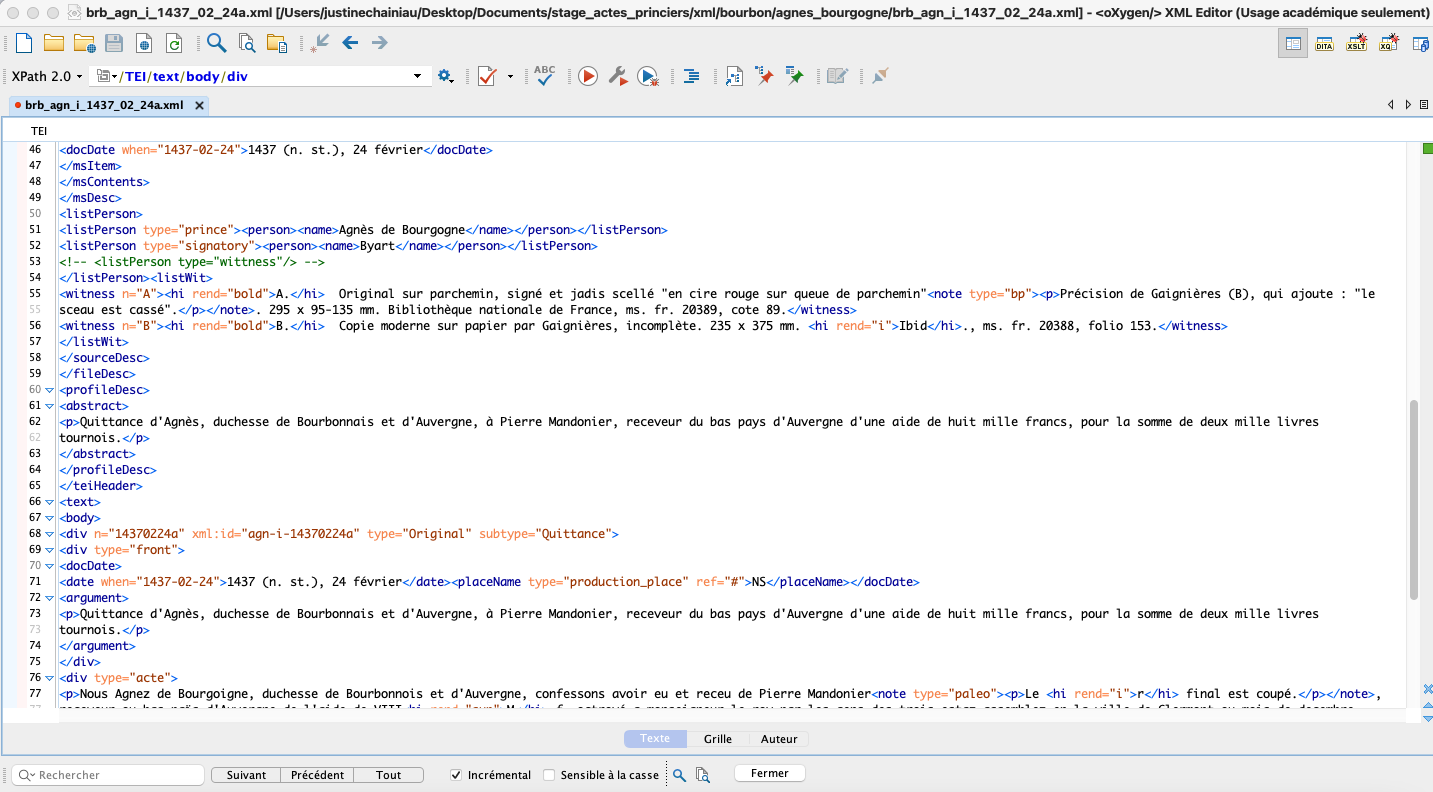
\includegraphics[scale=0.31]{img/fichier_indiv.png}
    \caption{Fichier XML de l'acte daté du 24 février 1437.}
    \label{fig:fichier_indiv}
\end{figure}
\newpage 

\par Les fichiers individuels sont pourvus d'un TEI Header complété d'informations générales, ajoutées à tous les actes. Le <Filedesc> comporte la description bibliographique du document. La balise <titleStmt> comprend plusieurs balises imbriquées correspondant à plusieurs niveaux de titre. Ensuite, la balise <editionStmt> présente le projet d'édition ainsi que les personnes en charge de celui-ci. Les indications sur la diffusion du fichier numérique et ses droits d’utilisation (licence) sont dans le <publicationStmt>. Les données individuelles, propres à chaque fichier et extraites du CSV sont placées dans le <sourceDesc>, qui décrit le document source. Cette balise contient les éléments d'identification, de conservation, de datation de l'acte ainsi que la liste des personnes concernées (signataires et prince à l'origine de l'acte) et le tableau de la tradition. Ces éléments sont suivis du <profileDesc>, qui fournit une description détaillée des aspects non bibliographiques, des informations contextuelles, notamment via l'analyse de l'acte en question. Le TEI Header est suivi de l'édition encodée pour chaque acte. 
\newline 

\par L'utilisation de Python via des fonctions a permis de manipuler les données et ainsi d'améliorer la structuration des documents. D'abord via l'extraction de données dans d'autres documents qui n'étaient pas au format XML (CSV), puis via la substitution des balises initiales issues de la conversion en des balises TEI standard, enfin par la séparation des fichiers XML obtenus en fichiers individuels. Ces étapes ont répondu à l'objectif fixé initialement, à savoir l'encodage des éditions des actes selon le schéma établi en amont, et sont préalables à la mise en ligne des documents. 

\newpage
\thispagestyle{empty}
\mbox{}
\newpage

\chapter{Préparation à la mise en ligne des données}

\vspace*{\stretch{1.3}} 
\par Ce chapitre présente les dernières étapes de la chaîne de traitement, préalables à la mise en ligne des données. Avant cette dernière, les fichiers XML sont uniformisés, et bénéficient de corrections individuelles, souvent manuelles, puis sont transformés en LaTeX via XSLT et compilés en PDF. L'objectif est de pouvoir relire les actes et d'y repérer les erreurs, sans avoir à ouvrir un à un les documents XML. LaTeX est un langage et un système de composition de documents largement employé par la communauté scientifique qui met l'accent sur la structure et le contenu du texte, en codant la mise en page des documents\footnote{\cite{LaTeXDMS}.}. 
\vspace*{\stretch{0.7}} 
\newpage 

\section[Transformation et compilation des fichiers]{Transformation du XML en LaTeX et compilation en PDF}
\label{III.6.1}

\par Le langage LaTeX sépare le fond de la forme en définissant sémantiquement le contenu via des commandes. Il permet une gestion automatique du référencement (gestion des différentes parties d'un ouvrage : chapitres, citations, notes ...) et une typographie de qualité\footnote{\cite{LaTeXDMS}.}. Pour l'édition d'actes, les différentes parties sont mises en valeur. Chaque acte édité est inséré dans un groupe. La date fait office de titre en gras, l'analyse figure ensuite en italique, puis viennent le tableau de la tradition et le contenu textuel. Toutes ces parties sont séparées par des commandes de mise en forme (espaces, sauts de lignes ...). 
\newline 

\begin{figure}[H]
    \centering
    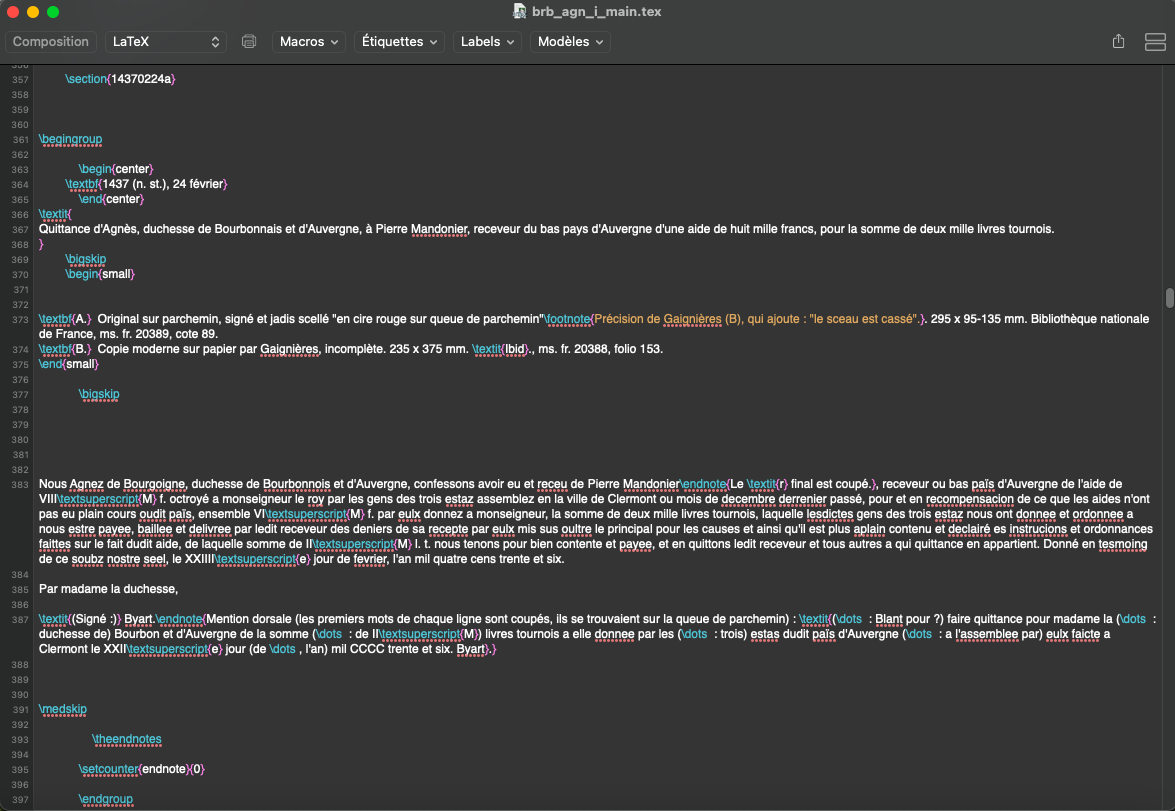
\includegraphics[scale=0.39]{img/latex.png}
    \caption{Fichier tex des actes d'Agnès de Bourgogne.}
    \label{fig:latex_agnes_db}
\end{figure}

\newpage 

\par L'objectif est d'assembler à nouveau tous les fichiers XML individuels obtenus pour chaque acte dans un seul fichier XML. La transformation de ce fichier en LaTeX permettra sa compilation et donc sa conversion et lecture au format PDF. Cela est réalisé grâce à une fonction Python\footnote{GitLab (py/compilation\_latex.ipynb).} qui transforme la langage XML en langage tex via XSLT. XSLT est le langage conçu pour transformer des documents XML en d’autres documents selon les spécifications XSL. XSL (eXtensible Stylesheet Language) désigne les spécifications pour écrire des feuilles de style, soit de quelle manière doivent être transformés les documents XML. Une fois le document correctement codé, une étape de compilation permet d'en produire un rendu final, ici un PDF mis en page. 

\begin{figure}[H]
    \centering
    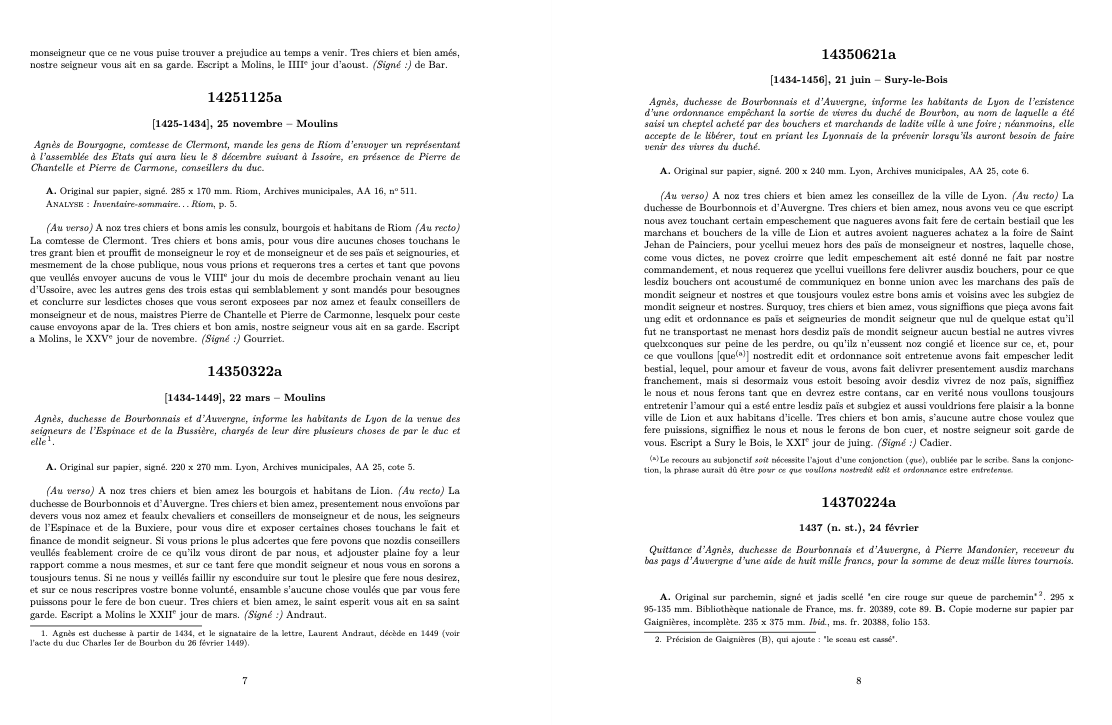
\includegraphics[scale=0.41]{img/pdf_compile_ab.png}
    \caption{Fichier PDF des actes d'Agnès de Bourgogne issu de la compilation du fichier tex.}
    \label{fig:pdf_conpile}
\end{figure} 

\par Les éditions une fois compilées en PDF rassemblent l'intégralité des actes pour chaque duc et duchesse. Chaque acte se distingue par son identifiant unique en gras et dans une taille plus importante. Ensuite, les dates de temps et de lieux apparaissent également en gras, séparées par une virgule. L'analyse en italique précède le tableau de la tradition, dont la numérotation des mentions est indiquée en gras. Puis vient le texte de l'acte, suivi des mentions hors teneurs indentées et du nom des signataires précédé de la mention \og (Signé:)\fg. Selon les cas, les notes paléographiques sont situées après le texte, en toutes petites capitales, alors que les notes de bas de page apparaissent en fin de page.  

\par La conversion du XML en tex permet la compilation puis une lecture agréable des éditions en PDF. L'ensemble de ces langages sont privilégiés par les travaux de recherche dans la mesure où ils assurent l'intégrité des données dans le temps. LaTeX est un logiciel libre, gratuit, multiplateforme et donc compatible avec différents systèmes d'exploitation et sans risque d'obsolescence. De plus, le programme est robuste, stable, compilé puisqu'il se met à jour lors de chaque compilation\footnote{\cite{LaTeX}.}. L'ensemble des technologies utilisées pour la transformation des documents permet donc la génération d'édition standard et mises en forme selon les \textit{Conseil pour l'édition de texte médiévaux} de l'École Nationale des Chartes\footnote{\cite{guyotjeanninConseilsPourEdition2009} \newline \cite{guyotjeanninConseilsPourEdition2014}.}. Toutefois, certaines erreurs de mise en page ont été repérées au sein des PDF. 
\newpage 

\section{Uniformisation des fichiers XML}

\par Après relecture des documents PDF générés, des anomalies figurent dans l'édition des actes\footnote{GitLab (medieval-acts/princely-acts/stage\_actes\_princiers\#7).}. Elles sont visibles et repérables au sein des PDF. Une fois identifiées, nous avons constaté qu'elles étaient souvent dues à des erreurs dans l'encodage des documents XML et à des erreurs de mise en forme. Les corrections sont effectuées au sein des fichiers individuels dans la mesure où les fichiers regroupant tous les actes pour chaque duc et duchesse, permettant par la suite la transformation en tex puis la compilation en PDF, sont générés à partir des fichiers individuels. Le mode projet d'Oxygen (l'éditeur XML) a permis de corriger ces écarts sur l'ensemble des fichiers individuels pour chaque prince, et même sur l'ensemble des quatre corpus, dans la mesure où il permet de naviguer dans l'arborescence du dossier XML du projet. 
\newline 

\par Les erreurs individuelles, propres à chaque corpus, ont été révisées en première intention. Le corpus de Louis II présente le plus d'anomalies.
L'une d'entre elles a été réglée directement via le script Python. Il s'agit de la suppression de la commande \og textsuperscriter \fg \space qui apparaissait dans la date de temps des actes datés du premier jour d'un mois. Le reste a été corrigé directement dans les fichiers XML. Premièrement, des regex ont été utilisées pour pallier les problèmes d'encodage. Les balises <hi> ne sont pas toujours encodées correctement. Certaines ne contiennent que des points ou une parenthèse. La mention \og signé \fg \space n'est pas continuellement insérée dans des balises <hi>, et est parfois fractionné. De plus, elle est parfois présente en double dans le document PDF, et n'est pas toujours indentée. Une centaine d'actes sont affectés par ces doubles mentions. En effet, elles sont ajoutées par XSLT, d'où la nécessité de les supprimer directement des XML via une regex. Les expressions régulières ont permis de remplacer les éléments (balises et leur contenu) incomplets par des éléments normalisés. Par ailleurs, une partie des défauts relevés dans les PDF proviennent des CSV. En effet, c'est par la ponction d'informations dans ces fichiers et leur ajout au XML que des éléments déficients se sont retrouvés par la suite dans le PDF. L'attribut de la balise <subtype> \og Traité-Accord \fg \space qui indique le type diplomatique de l'acte et atteste d'un accord passé entre plusieurs princes correspond en fait à des lettres patentes\footnote{AN, P 1357\up{2}, n°425 (13 août 1377). - AN, P 1370\up{2}, c. 1920 (21 avril 1386).}. Cet élément n'avait pas été revu dans le CSV des actes de Louis II et a ainsi été ajouté comme attribut de la première balise <div> dans les fichiers XML. À l'instar des XML, les fichiers CSV ont également bénéficié d'une révision, en supprimant et en remplaçant les mentions défaillantes par les mentions correctes via des regex. 
\newpage 

\par Deuxièmement, il est possible de corriger certains éléments en utilisant le Xpath, le chemin qui permet de naviguer au sein de l'arbre XML. Des points d’interrogations, qui marquaient des incertitudes sur les types diplomatiques dans les CSV, ont été relevés au sein des balises <subtype> et <type>, puis éliminés. Troisièmement, les erreurs singulières ont été corrigées manuellement. C'est le cas d'une date de temps qui était doublée (acte daté du vingt-deux septembre puis signé le vingt-sept septembre) et encodée dans la date de lieu\footnote{AN, P 1357\up{2}, n°442 (22 et 27 septembre 1399).}. Une référence a aussi été trouvée dans une date de lieu. Le corpus d'Anne Dauphine ne comporte quant à lui qu'une date de temps encodée dans une date de lieu, qui a également été retirée manuellement. 
\newline 

\par Le corpus de Charles I\up{er} comporte une erreur majeure due au remplissage du CSV, qu'il est possible de corriger via une regex. Le type diplomatique n'est pas normalisé : on retrouve la mention \og dep \fg \space au lieu de \og deperditum \fg. Les expressions régulières ont permis le remplacement instantané des cent trente-trois occurrences à la fois dans le CSV et dans les fichiers XML. Le corpus d'Agnès de Bourgogne n'est pas non plus exempt d'erreurs d'encodage. En effet, la plupart des dates de lieu des actes sont encodées dans la balise <date>. Ainsi, seules des mentions \og NS \fg \space sont encodées dans la balise <placeName>. En conséquence, lors de la transformation, les mentions \og NS \fg \space ne sont pas interprétées et la date de temps et la date de lieux ne sont donc pas séparées par des tirets dans le PDF puisqu'elles sont encodées dans la même balise. Cela a été corrigé manuellement dans la mesure où les actes concernés n'étaient pas trop nombreux.
\newline 

\par Les problèmes de mise en page généraux, qui concernent les quatre corpus, sont résolus à la fin grâce à l'emploi de regex. C'est le cas des lignes vides entre la balise fermante <listwist> et la <div> suivante, ainsi que des nombreux retours à la ligne après et avant les notes, qui ont été éliminés. Parfois, la numérotation des états du texte est signalée en gras : \og \textbf{A.}\fg \space de manière complètement aléatoire. Or, les numéros (A, B, C) d'exemplaires doivent tous être en gras. Une regex a permis de les attraper et de les styler uniformément. Des opérations d'harmonisation des fichiers XML ont été décidées, comme l'homogénéisation des dénominations des services d'archives. Par exemple, \og Archives municipales de Montluçon \fg \space devient \og Montluçon, Archives municipales \fg. La \og Bibliothèque municipale de Lyon \fg \space est remplacée par \og Lyon, Bibliothèque municipale \fg. Les \og Archives départementales de la Loire \fg \space deviennent \og Archives départementales Loire\fg. Pour les Archives nationales, on indique \og Paris, Archives nationales \fg. Cet alignement nécessite une réflexion conjointe des chercheurs travaillant sur le projet en amont, afin de se mettre d'accord sur des standards, et de les communiquer ensuite afin qu'ils soient respectés lors des prochains ajouts au projet.
\newpage 

\par Les dénominations des lieux bénéficient également d'une harmonisation. Certaines dates de lieu comportent des parenthèses dont l'usage n'est pas justifié : Bourbon(-l’Archambault), Clermont (en Auvergne). Des actes comportent parfois la mention \og (château de) \fg \space ou \og au château \fg \space après la date de lieu. Nous avons convenu que les toponymes seraient retranscrits en entier sans parenthèses. Toutefois, lorsqu'il y a une précision en plus de la ville, celle-ci doit figurer entre parenthèses : Moulins (Château), Paris (Hôtel de Bourbon), Riom (Palais). Certaines étapes plus précises n'ont pu être effectuées automatiquement. Lorsqu'il y a au sein d'une édition une référence à un acte qui était auparavant numéroté (ex : cf. acte n°XX), cette référence est remplacée par l'identifiant du fichier XML de l'acte en question. Les actes sans mesures du corpus de Louis II ont également été repérés en vue de compléter les balises <witness> dans la mesure du possible. 
\newline 

\par L'emploi de regex et le recours au Xpath ont permis d'automatiser un certain nombre d'opérations visant à améliorer et à homogénéiser le plus possible l'encodage des actes. Toutefois, des opérations n'ont pu être automatisées et certaines choses n'ont pas pu être corrigées en raison de leur complexité. C'est le cas de la balise <witness> qui n'est en définitive pas aussi structurée que sur le schéma théorique comme balise parent des balises <text>, <orgname>, <idno1>, <idno2>\footnote{Figure 5.3 – Schéma d’encodage des actes en XML.}. Les mentions hors teneur ne sont pas dotées non plus d'un attribut \og subtype\fg \space indiquant leur positionnement. Néanmoins, les étapes précédentes tendent à rendre la structuration des fichiers XML la plus uniforme possible pour leur mise en ligne. 
\newpage 

\section{Encodage d'actes inédits}

\vspace*{\stretch{0.4}} 
\par Après avoir détaillé la chaîne de traitement des données, se pose la question des actes inédits. Au vu de la dispersion du corpus, nous ne sommes pas à l'abri de découvrir des actes passés au nom des ducs de Bourbon qui auraient échappé à notre recensement. Comment intégrer de nouveaux actes au corpus ? Une partie de la réponse à cette question a été développée en amont. En effet, le schéma d'encodage précis établi précédemment détaille la procédure à suivre pour encoder de nouvelles données afin qu'elles soient conformes au corpus\footnote{CANEVAS TEI, dans Chapitre 5, 5.3. Séparation des fichiers XML de corpus en fichiers XML d’actes}. Nous avons expérimenté ce procédé avec l'intégration des actes de Charles~I\up{er} repérés aux archives\footnote{AN, P 4522, c. 190 (24 octobre 1443) - AN, P 4522, c. 307 (24 octobre 1443) - AN, P 4522, c. 313 (24 octobre 1443) - AN, P 4522, c. 229 (25 octobre 1443) - AN, P 4522, c. 169 (22 octobre 1454), dans chapitre 2, 2.3 Le traitement de texte : un bon compromis ?}. Dans un premier temps, le travail a lieu sur place. Il s'agit de photographier et de mesurer les actes en question. Les prises de vues permettront par la suite d'analyser les actes et d'alimenter le site web. Cinq actes ont été repérés dans le registre P 452\up{2}, pour Charles I\up{er}. Les séries P 452 et 453 renferment les documents relatifs au bourbonnais, plus précisément les anciens hommages, effectués entre 1355 et 1530\footnote{Archives Nationales, \og Série P Chambre des comptes et comptabilité\fg, en ligne : \url{http://www.archivesnationales.culture.gouv.fr/chan/chan/fonds/EGF/SA/SAPDF/Egfn-p.pdf}.}. Les actes concernés sont respectivement datés du vingt-quatre octobre 1443 pour trois d'entre eux, du 25 octobre 1443 et du 22 octobre 1454\footnote{Annexe Actes inédits.}. Les cinq actes attestent de l'hommage d'individus du duché pour leurs possessions dans celui-ci : Jean Chauvet, Jean de Meschatain, Pierre de Saint Aubin, Jean de Bar et Jean de la Porte. 
\vspace*{\stretch{0.2}} 
\newpage 

\begin{figure}[H]
    \centering
    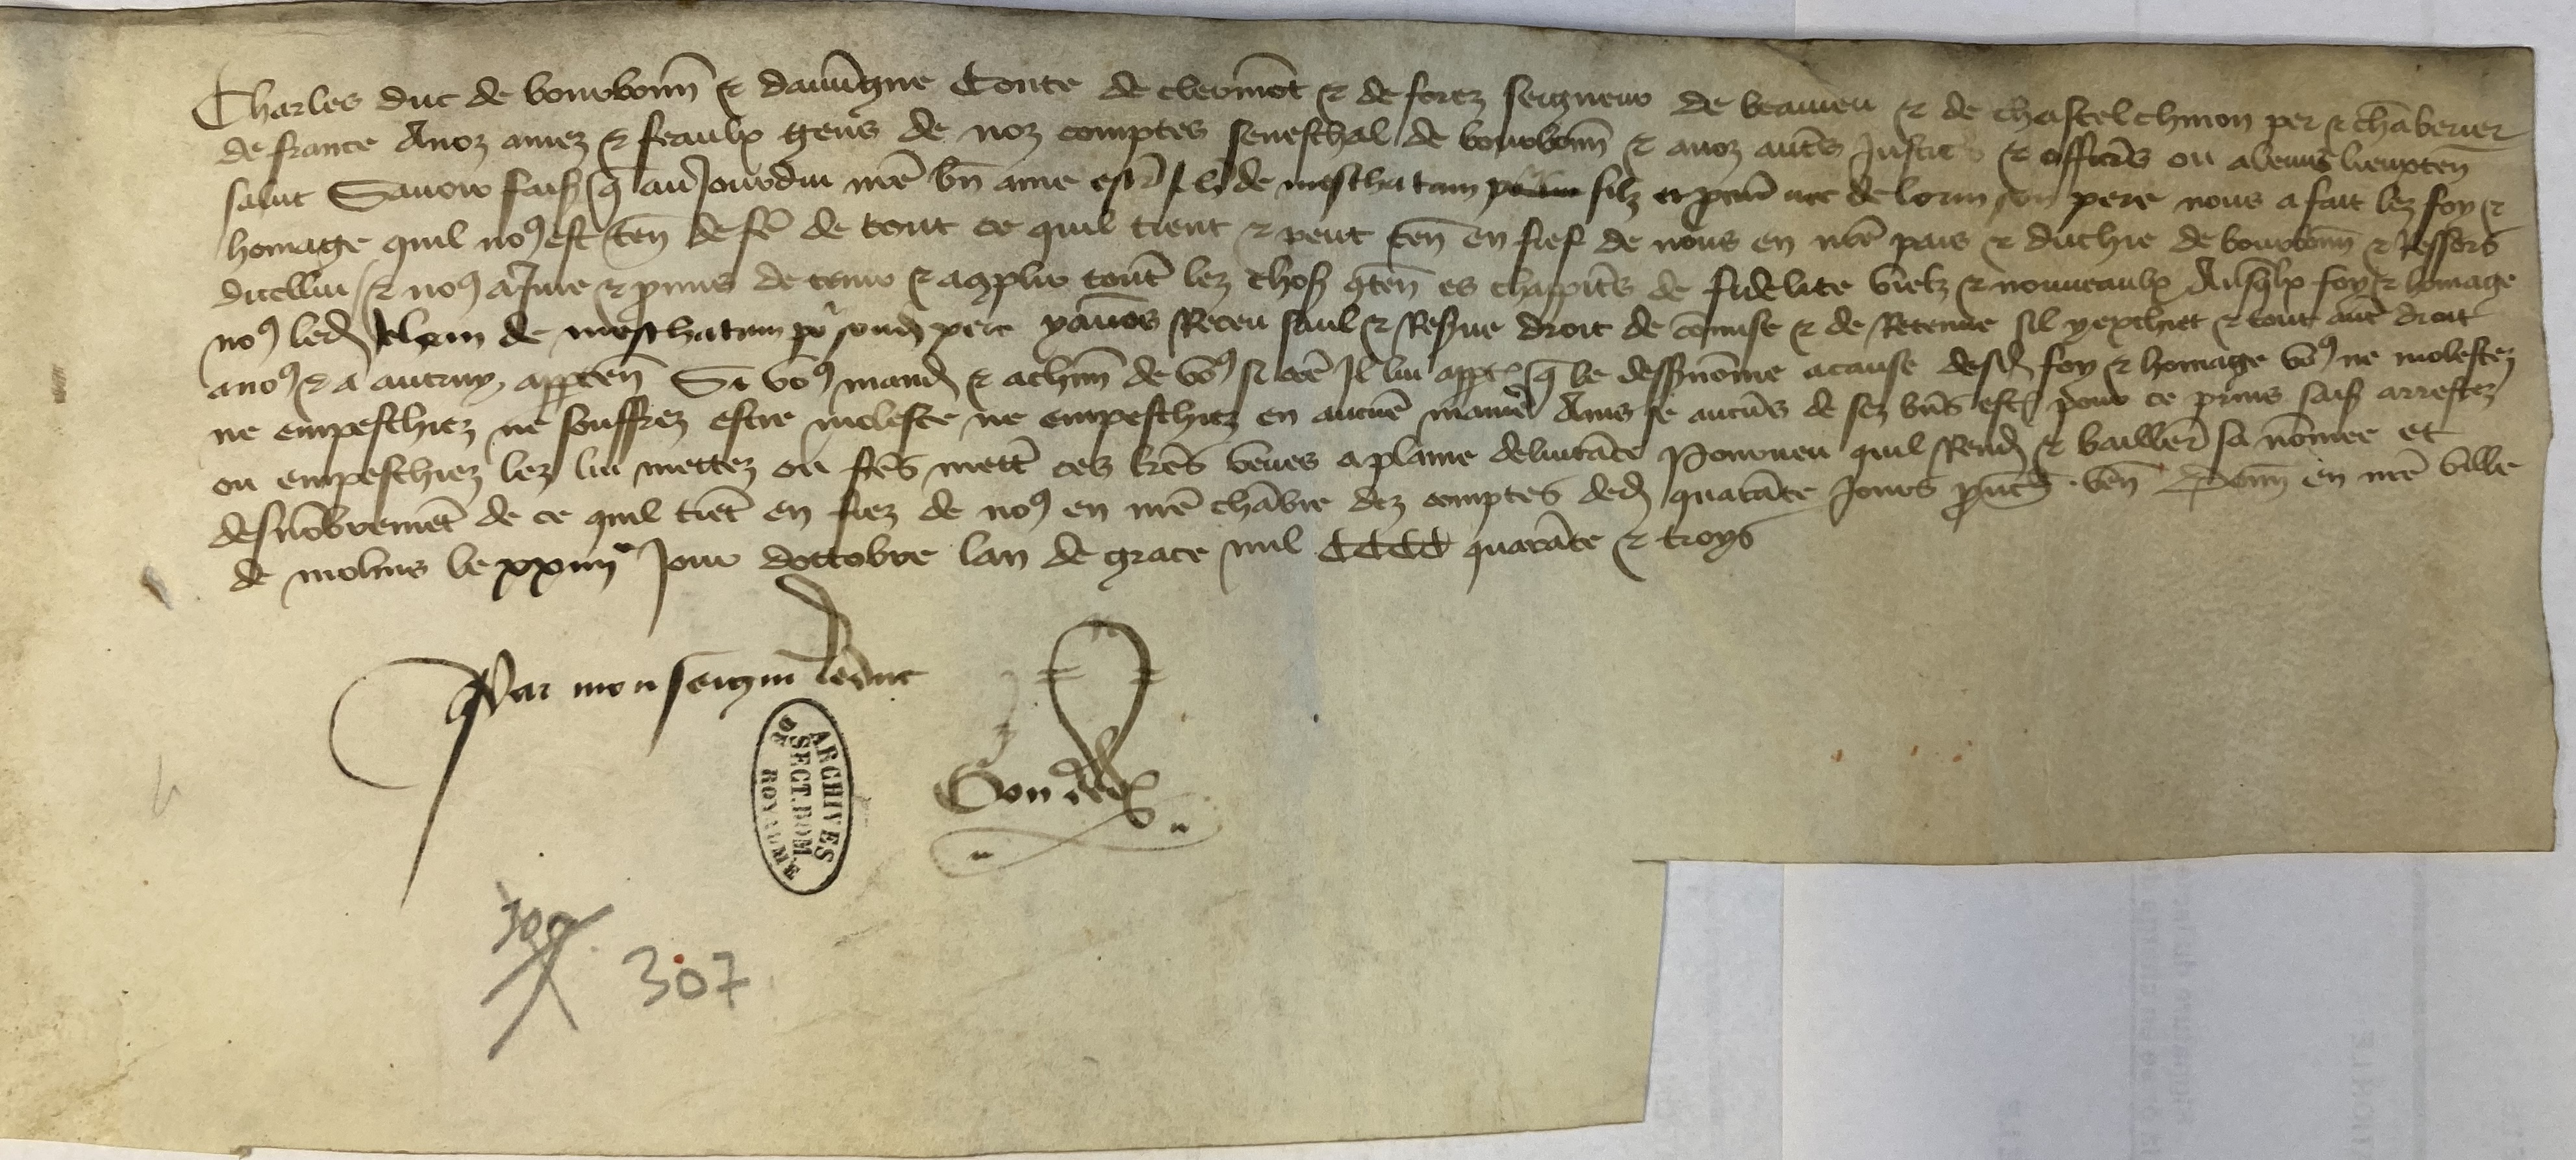
\includegraphics[scale=0.115]{img/1443_10_24b.jpg}
    \caption{Photographie de l'acte daté du 24 octobre 1443. \newline Charles, duc de Bourbonnais et d'Auvergne, etc., notifie aux gens de ses comptes qu'il a reçu l'hommage de Jean de Meschatain pour tout ce que celui-ci tient de lui en fief dans le duché de Bourbonnais.}
    \label{fig:1443_10_24b}
\end{figure} 

\par À partir des photographies prises, les actes sont transcrits selon les normes développées dans les \textit{Conseils pour l'édition des textes médiévaux}\footnote{\cite{guyotjeanninConseilsPourEdition2009}.}. La transcription donne accès au contenu du texte et à des informations essentielles comme la datation, le lieu de rédaction, ou encore des noms d'individus, qui vont permettre de compléter le schéma XML. La deuxième étape consiste à encoder l'acte. La transcription peut avoir lieu directement à cette étape si le texte n'est pas trop difficile à lire\footnote{Encodage des actes concernés : Gitlab \newline (xml/bourbon/charles\_i\_bourbon/brb\_ch\_i\_1443\_10\_24a.xml), \newline (xml/bourbon/charles\_i\_bourbon/brb\_ch\_i\_1443\_10\_24b.xml), \newline (xml/bourbon/charles\_i\_bourbon/brb\_ch\_i\_1443\_10\_24c.xml), \newline (xml/bourbon/charles\_i\_bourbon/brb\_ch\_i\_1443\_10\_25a.xml), \newline (xml/bourbon/charles\_i\_bourbon/brb\_ch\_i\_1454\_10\_22a.xml).}. Le TEI Header est complété avec des informations d'identification de l'acte. La date est nécessaire pour remplir l'attribut \og xml:id \fg \space de la balise <TEI> ainsi que le titre de niveau \og a \fg. Ensuite, c'est tout le contenu de la balise <sourceDesc>, décrivant le document, soit l'acte concerné, qui est à remplir avec les identifiants de l'acte : institution de conservation, fonds, cote ainsi que sa date de rédaction. Puis, viennent la liste des personnes mentionnées : prince à l'origine de l'acte et signataire. Enfin, le <sourceDesc> est complété par le tableau de la tradition. Le <profileDesc> contient les informations contextuelles, soit un résumé en quelques mots de l'acte en question. 
\newpage

\par Une fois le TEI Header complété, c'est le <text> avec les attributs de la première <div> : identifiants, état, type diplomatique. Les balises enfant de la balise <docDate> sont enrichies des dates de temps et de lieu. Ensuite, l'analyse précède le texte transcrit. Le texte de l'acte est retranscrit tel quel et les lettres et les graphies manquantes ou erronées sont déclarées au sein de l'apparat critique. Des balises signalent les personnes et les lieux du texte. Ces deux derniers éléments, ainsi que le signataire, qui clôt le texte, sont référencés. 
\newline 

\begin{figure}[H]
    \centering
    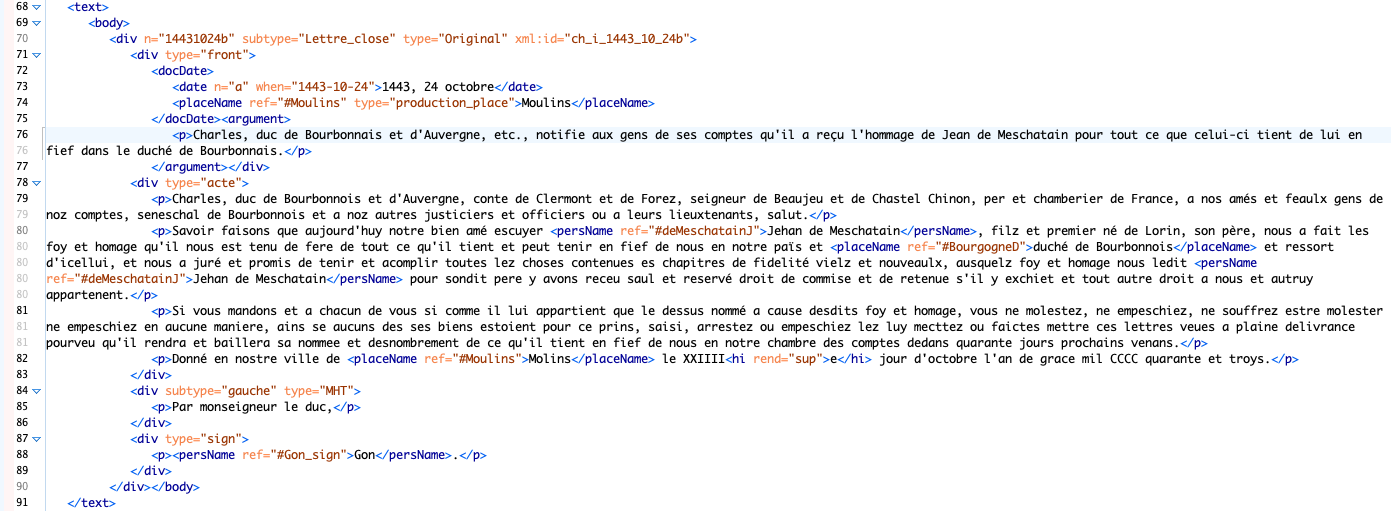
\includegraphics[scale=0.33]{img/encodage_text.png}
    \caption{Encodage TEI du texte de l'acte daté du 24 octobre 1443.}
    \label{fig:encodage_1443}
\end{figure} 

\par Toutes les étapes préalables à la mise en ligne des données détaillées dans les sections précédentes sont réplicables, ce qui rend possible l'élargissement du corpus lorsque de nouveaux actes de même nature sont découverts. En effet, il est possible de relancer les scripts afin d'assurer la transformation en LaTeX et la compilation en PDF du corpus, une fois les nouveaux actes encodés en XML, et ainsi les ajouter aux éléments déjà mis en ligne. Toutefois, ce procédé fonctionne et représente un gain de temps pour des corpus édités sur du traitement de texte et dont les inédits ne sont pas trop nombreux à ajouter. Afin de traiter des corpus qui n'auraient pas été édités, il serait plus pertinent de fragmenter le texte des actes et les informations le concernant, nécessaires à l'élaboration d'une édition, pour les intégrer à une base de données, qui, parsée par un script Python, pourrait permettre de générer un encodage en XML\footnote{Cette méthode est développé dans : \cite{devaleriolaOrdinateurAuService2020}.}. 

\newpage
\thispagestyle{empty}
\mbox{}
\newpage
    
    \backmatter\chapter{Conclusion}

\par La mobilisation de techniques numériques a permis de faciliter l'étude des corpus conséquents et dispersés que sont ceux de Louis II, d'Anne Dauphine, de Charles I\up{er} et d'Agnès de Bourgogne. 
\newline 

\par Le présent mémoire s'est attaché à présenter les documents étudiés : datation, typologie, dispersion, similitudes des actes des ducs de Bourbon. Nous sommes également revenus sur la manière dont ces derniers ont été traités initialement, car le projet d'encodage des actes pour la mise en ligne ne part pas de rien. En effet, les actes ont d'abord été édités avec un logiciel de traitement de texte. Nous avons alors développé une chaîne de traitement des documents à partir des éditions utilisées comme \textit{legacy data}. Ensuite, nous avons travaillé sur les documents afin de les préparer à l'encodage en XML/TEI. Cette étape s'est articulée autour d'une proposition de méthode de stylage des éditions en vue d'une conversion, puis du choix d'un convertisseur approprié. Puis, après conversion des documents, plusieurs scripts Python ont facilité les interventions sur les éditions de façon à améliorer et affiner leur structuration. Ces étapes ont également permis d'extraire et d'ajouter des données. Enfin, les fichiers ont été préparés à la mise en ligne via la génération d'un fichier XML pour chaque acte, puis une compilation en PDF (via une transformation en LaTeX). Ces dernières étapes ont rendu visibles les anomalies et possibles les corrections sur le document et initié la réflexion sur le projet (intégration d'actes inédits ...). 
\newline 

\par Toutes les opérations de traitement des actes explicitées dans ce travail peuvent être qualifiées de semi-automatiques, dans la mesure où il y a une alternance entre des traitements automatiques et des traitements manuels. Sébastien de Valeriola insiste sur la complémentarité de ces deux méthodes en affirmant que \og le travail de la machine ne remplace aucunement celui de l’historien, mais l’accompagne et le facilite \fg \footnote{\cite{devaleriolaOrdinateurAuService2020}.}. L'enjeu de ce travail sur le projet \og Actes Princiers \fg \space était d'automatiser ce qui pouvait l'être. Comme nous partions d'éditions réalisées avec un logiciel de traitement de texte, de nombreuses opérations ont été semi-automatiques, comme le stylage des actes via des regex en première intention et manuel pour les cas les plus compliqués. L'ordinateur est un bon outil pour réaliser les traitements les plus volumineux comme la transformation en XML et la séparation des corpus de chaque prince en fichiers individuels. Cette automatisation évite les erreurs humaines d'encodage dans notre cas. Mais, il est nécessaire de contrôler l'issue de ces manipulations, car il est fréquent que la machine bute sur des erreurs antérieures. L'automatisation permet également de rendre applicable le processus de traitement des données à l'avenir à d'autres actes et éventuels corpus. Toutefois, malgré sa réplicabilité, l'ensemble d'opérations développé est adapté à un corpus relativement homogène. Il ne faut pas perdre de vue qu'il est difficile de proposer une méthodologie cohérente, car même en suivant un modèle d'édition précis et reconnu, on ne peut pas prévenir toutes les individualités inhérentes à la recherche. L'enjeu reste donc de tendre au plus uniforme possible.
\newline 

\par L'uniformité, lorsqu'elle est atteinte, ou du moins approchée au maximum, entraîne une automatisation accrue des procédés de traitement des données et facilite ainsi l'extraction d'un maximum d'informations des corpus. Dans ce sens, la méthode de stylage des documents pourrait être encore affinée et couplée à de la diplomatique en distinguant les différentes parties de l'acte (intitulation ...), afin d'étudier leurs caractéristiques via des méthodes quantitatives et ainsi de comparer les formules utilisées, la rédaction et l'utilisation de modèles dans certains cas ou encore l'évolution des pratiques d'écriture. Des études prosopographies pourraient également être développées à partir des personnes référencées dans chaque corpus et ainsi mettre en lumière des réseaux sociaux. En effet, les actes sont riches en renseignement sur les acteurs dans la mesure où ils mentionnent souvent une activité, un lieu d'habitation, parfois des relations. Plus largement, le site pourrait être enrichi d'autres corpus. Dans un premier temps, ceux de Jean I\up{er} et de Marie de Berry pourraient bénéficier d'un travail dans la mesure où ils n'ont pas encore été très approfondis et où il serait pertinent de faire le lien entre les deux périodes de ducat de Louis II et de Charles I\up{er}. Cela permettrait aussi d'étudier l'administration du duché pendant la période particulière que fut celle de la captivité du duc, en pleine guerre de Cent Ans. 
\newline 

\par Le projet \og Actes Princiers\fg \space et les travaux menés dessus donnent l'impulsion aux recherches sur les actes des princes du royaume de France. Enfin, ce type de projet rend les données disponibles sur le web et accessibles à la communauté scientifique en proposant des \textit{legacy data} homogènes et facilement exploitables et contribue ainsi à une meilleure connaissance de la diplomatique princière pour la période étudiée.

\newpage
\thispagestyle{empty}
\mbox{}
\newpage

    \appendix\chapter{Annexes}

\section*{Chronologie des éditions}
\addcontentsline{toc}{section}{Chronologie des éditions}

\begin{figure}[ht]
    \centering
    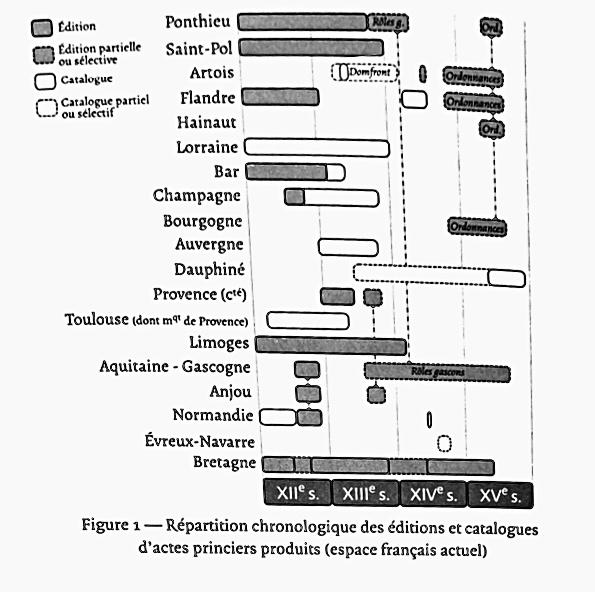
\includegraphics[scale=0.6]{img/repartition_chronologique_editions.jpeg}
    \caption*{Canteaut, Olivier, Moufflet, Jean-François, « Les éditions d’actes princiers (\textsc{XII}\up{e} - \textsc{XV}\up{e} siècle) : bilan à l’ère du numérique », in : Olivier Guyotjeannin et Olivier Mattéoni (éd.), Jean de Berry et l’écrit : Les pratiques documentaires d’un fils de roi de France, Éditions de la Sorbonne, École Nationale des Chartes, Paris, 2019 (Histoire ancienne et médiévale, 159).}
    \label{fig:chrono_ed}
\end{figure}

\section*{Généalogie de la famille ducale de Bourbon}
\addcontentsline{toc}{section}{Généalogie de la famille ducale de Bourbon}

\begin{figure}[H]
\centering
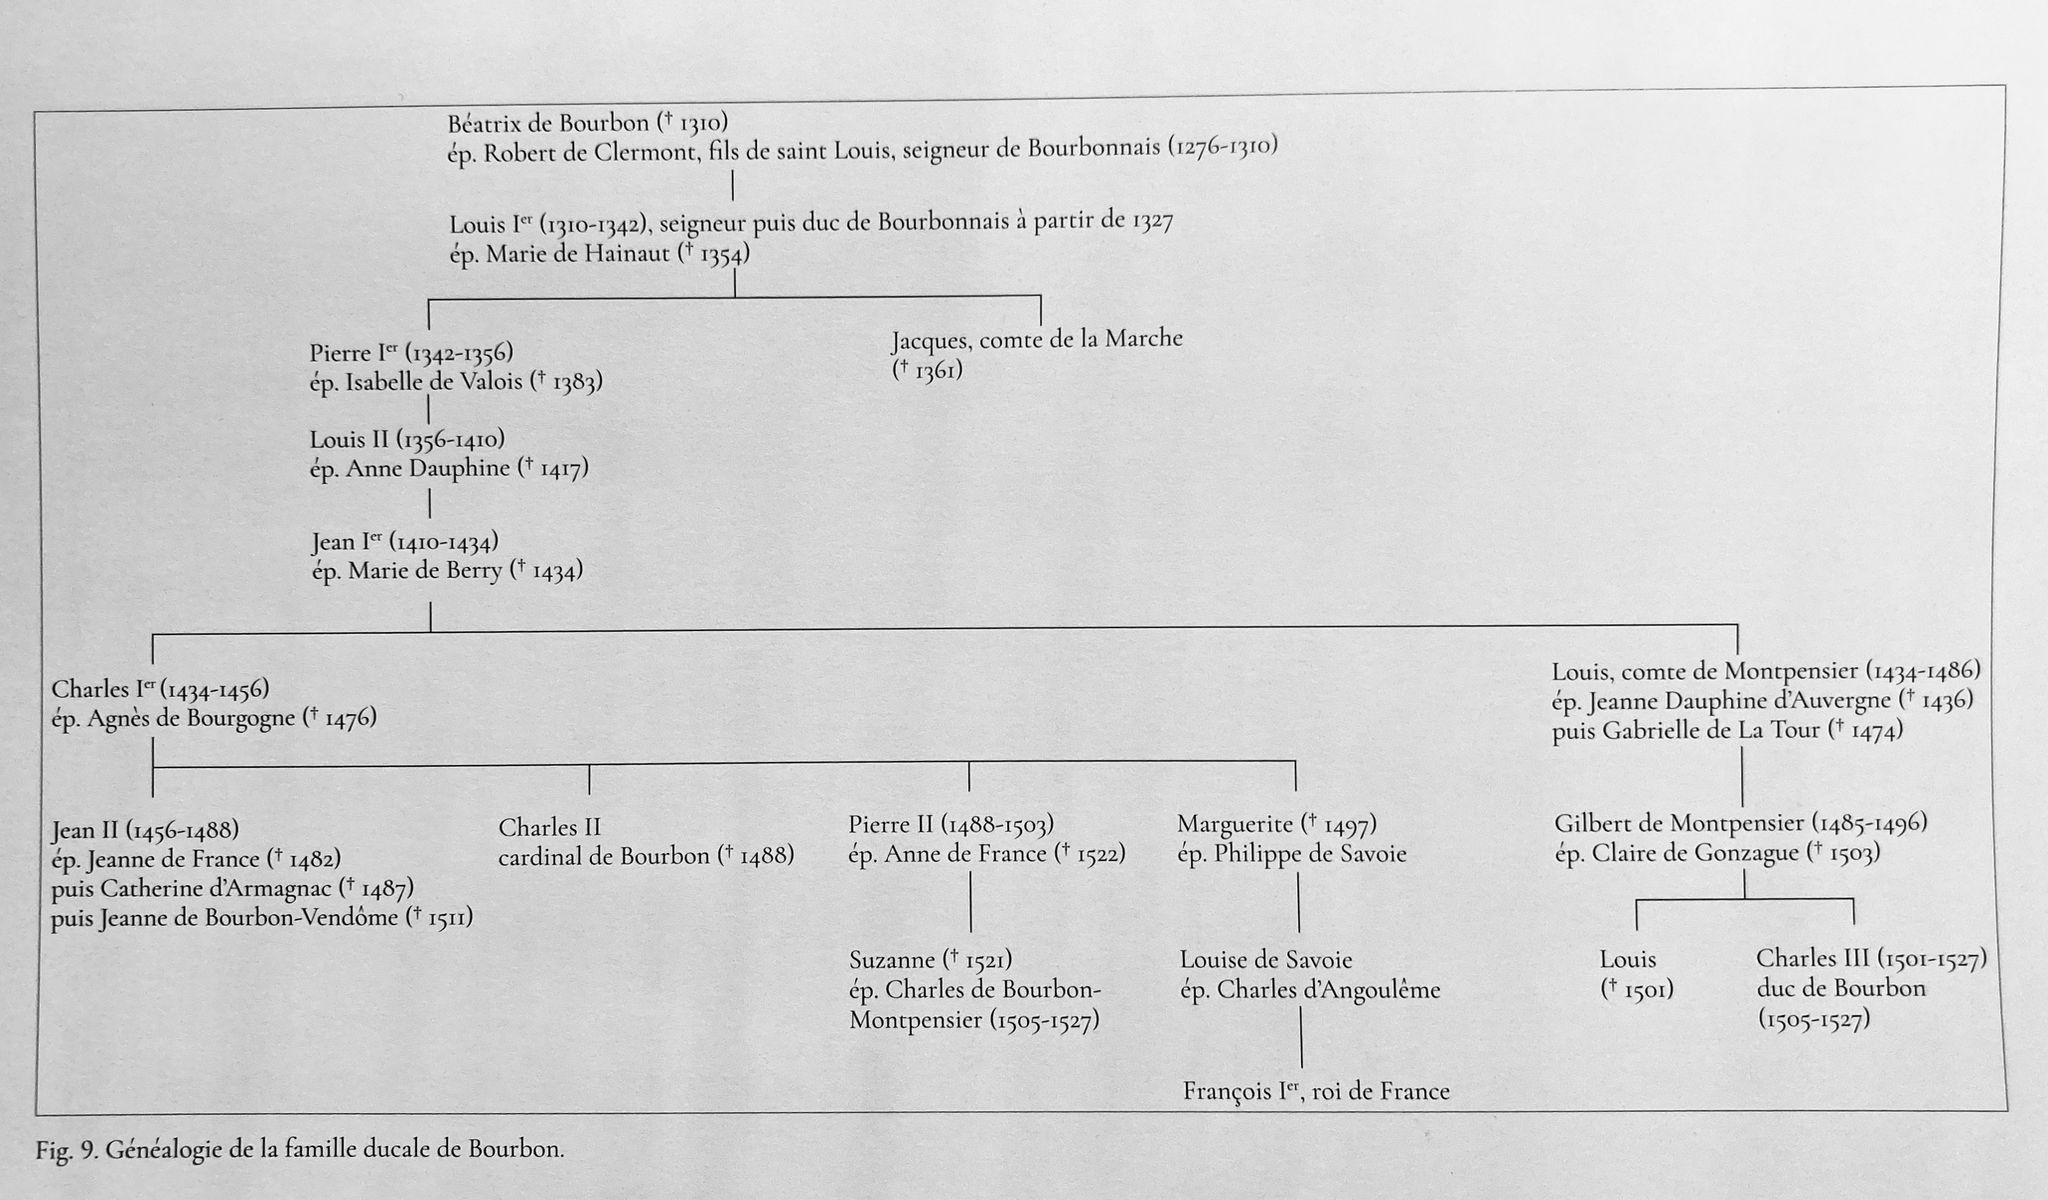
\includegraphics[scale =0.22]{img/genealogie.jpeg}
\caption*{Généalogie de la famille ducale de Bourbon, in \cite{matteoniBourbonsLeurBibliotheque2022}.}
\label{genealogie}
\end{figure}
\newpage 

\section*{Initiales fleurdelisées}
\addcontentsline{toc}{section}{Initiales fleurdelisées}

 \begin{figure}[H]
\centering
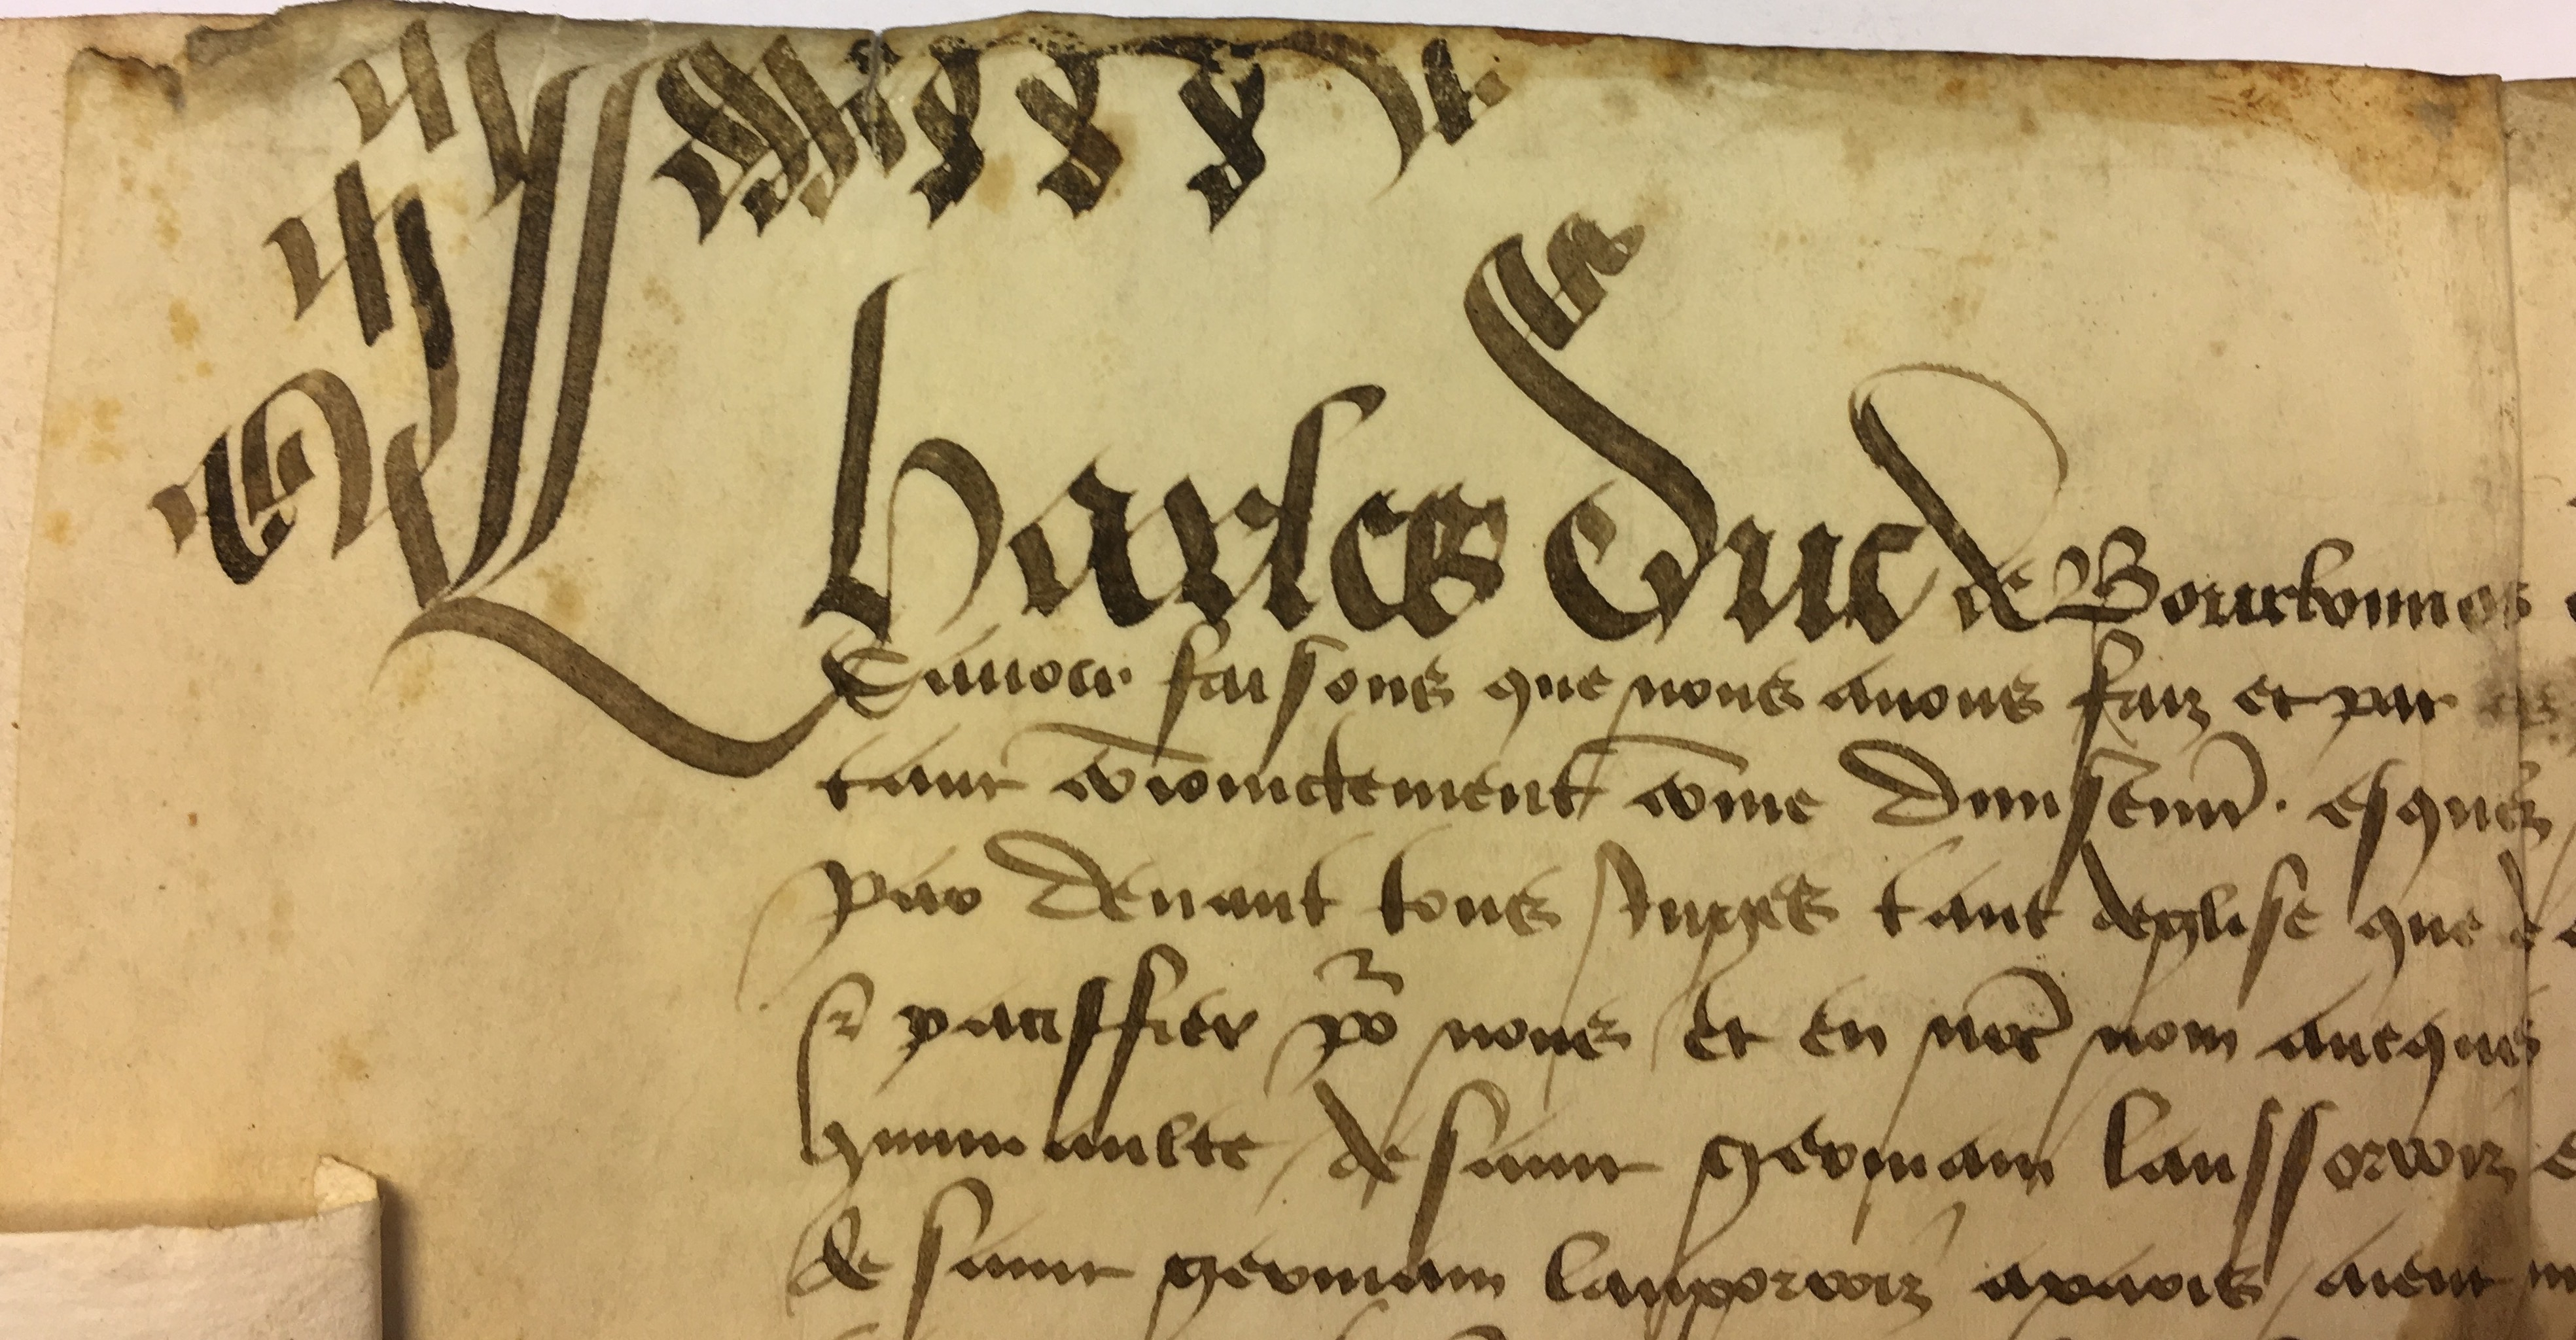
\includegraphics[scale =0.09]{img/fleurlys1.jpg}
\caption*{AN, P 13631, c. 11511 (18 décembre 1448).}
\label{fl1}
\end{figure}

\begin{figure}[H]
\centering
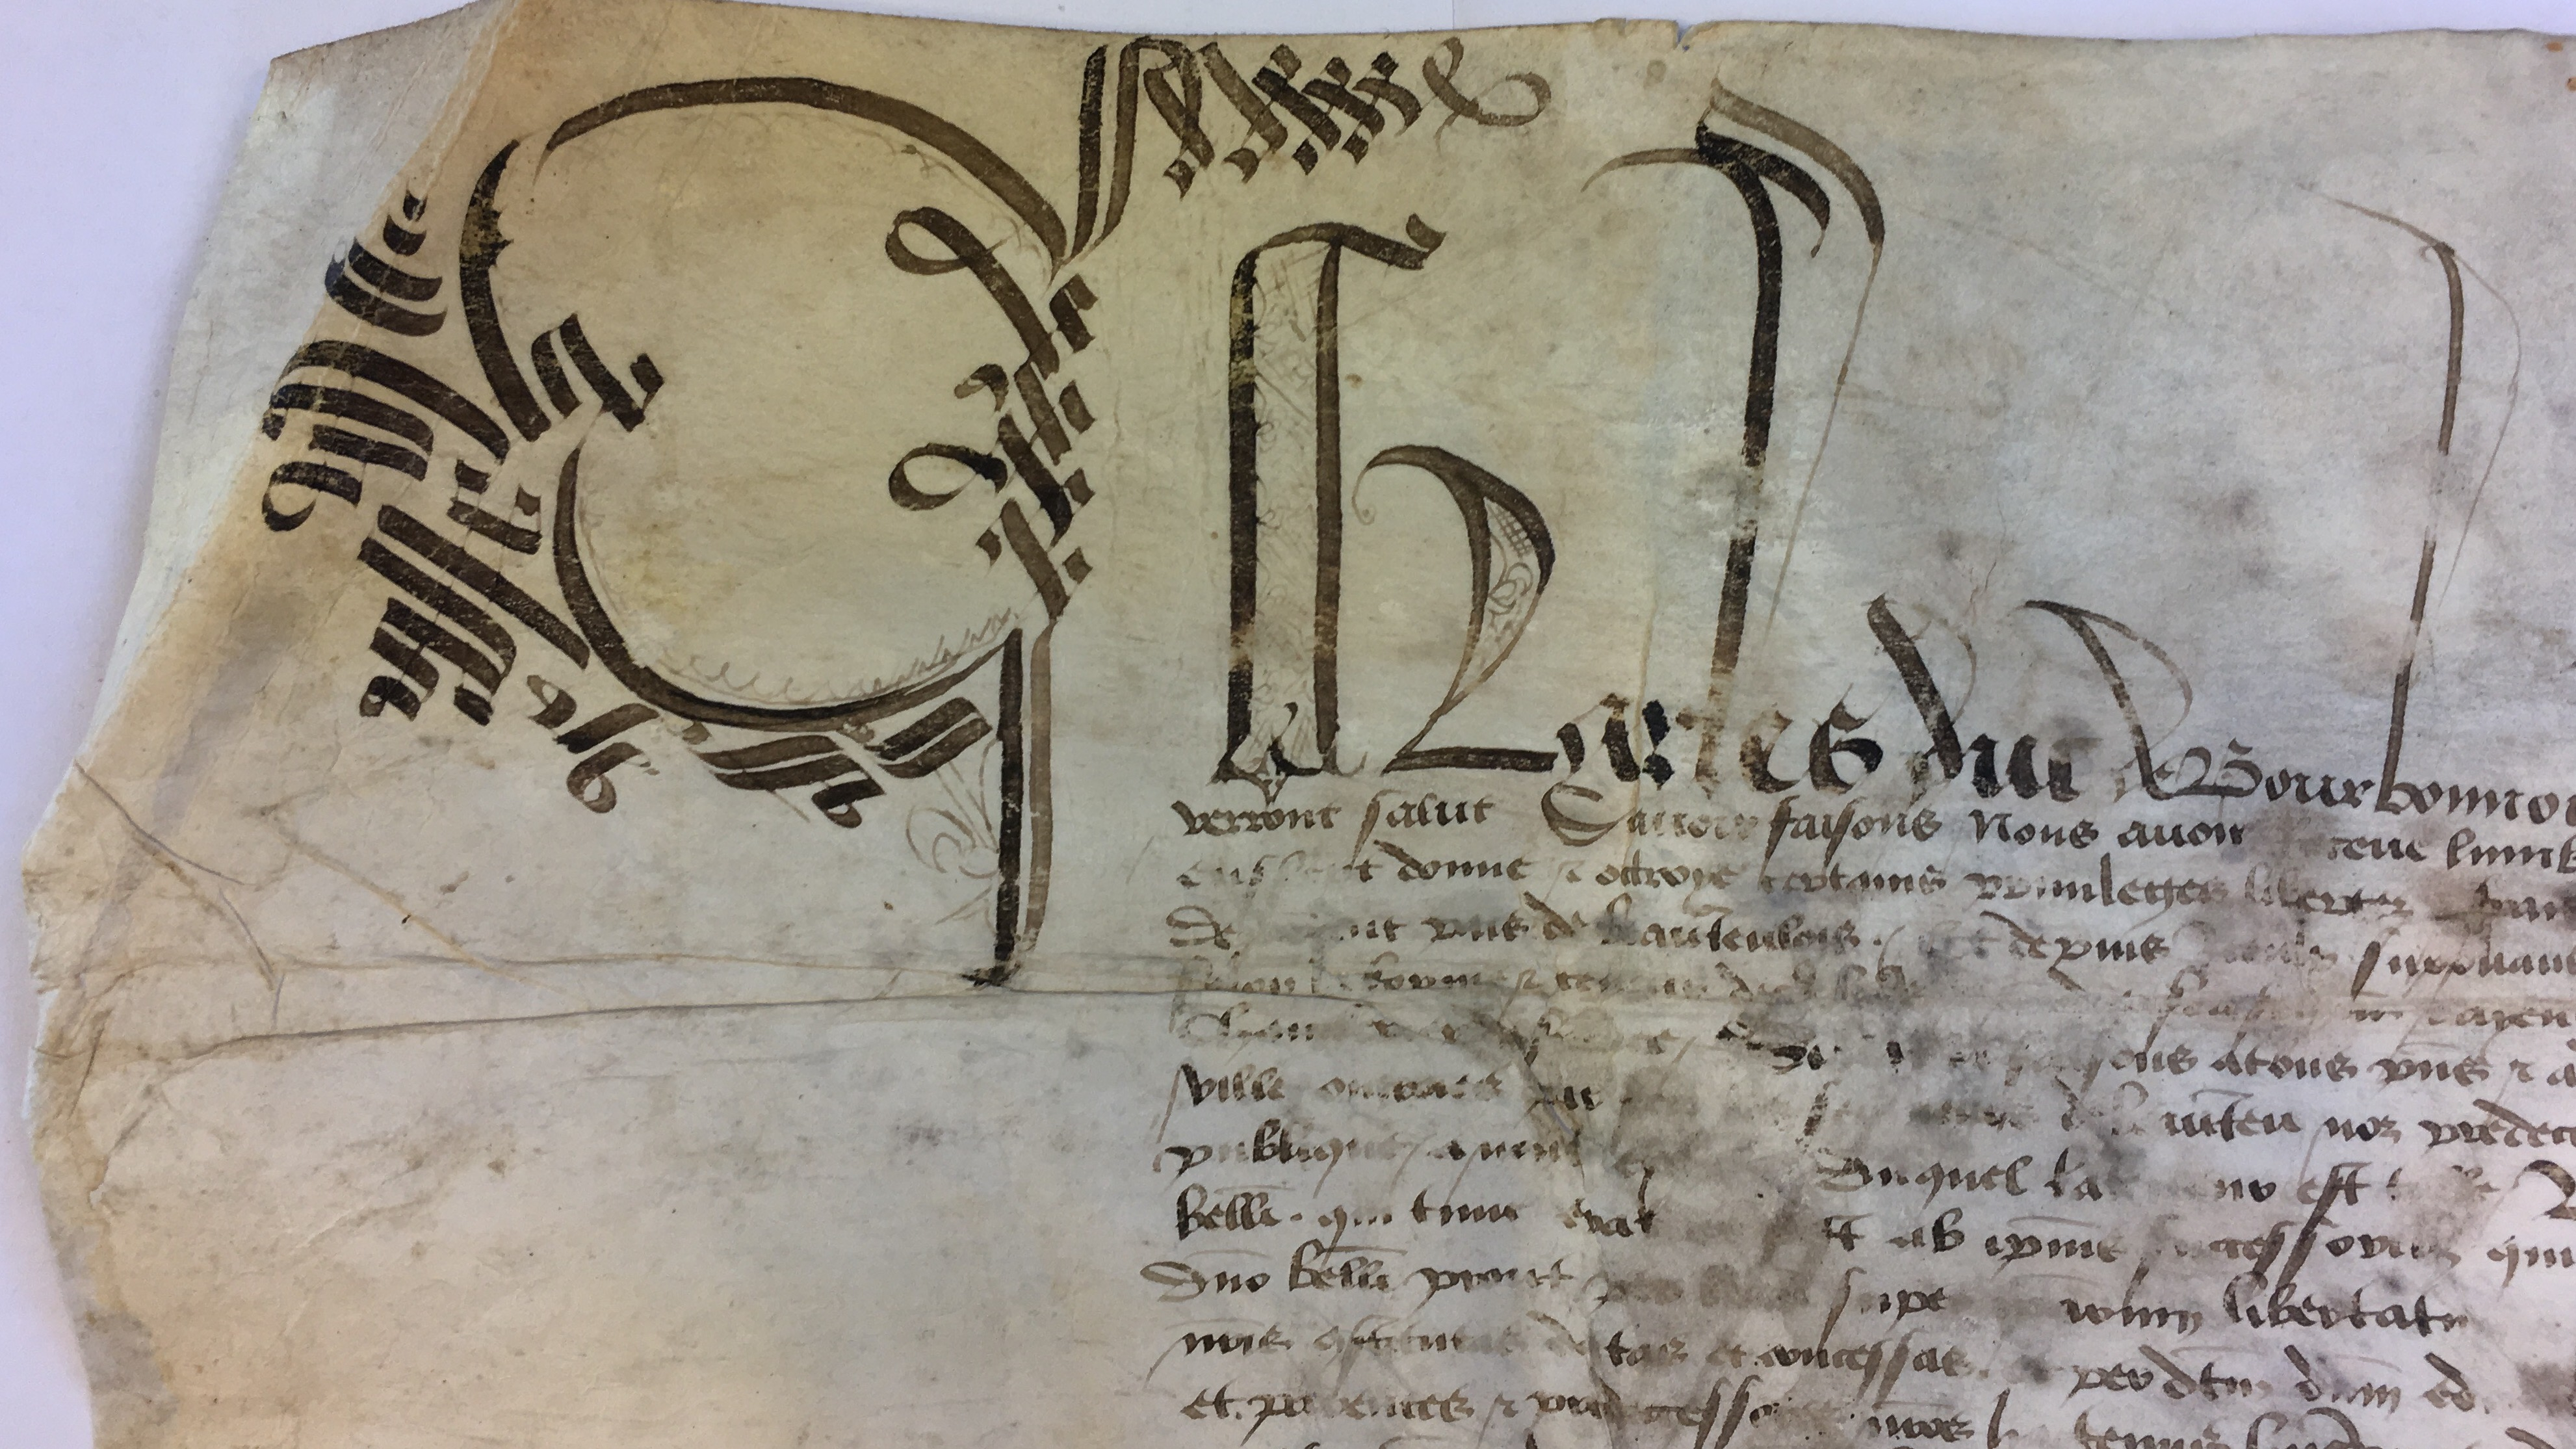
\includegraphics[scale =0.09]{img/fleurlys2.jpg}
\caption*{AN, P 13682, c. 1628 (19 février 1447).}
\label{fl2}
\end{figure}
\newpage 

 \section*{Liste des regex utilisées}
 \addcontentsline{toc}{section}{Liste des regex utilisées}
 
\begin{center}
\begin{longtable}{|l|l|l|}

\hline 
\multicolumn{1}{|c|}{\textbf{Action}} & \multicolumn{1}{c|}{\textbf{Regex}} & \multicolumn{1}{c|}{\textbf{Remplacement}} \\ \hline 
\endfirsthead

\multicolumn{3}{c}%
{{\bfseries \tablename\ \thetable{} -- Liste des regex utilisées}} \\
\hline \multicolumn{1}{|c|}{\textbf{Action}} & \multicolumn{1}{c|}{\textbf{Regex}} & \multicolumn{1}{c|}{\textbf{Remplacement}} \\ \hline 
\endhead

\hline \multicolumn{3}{|r|}{{}} \\ \hline
\endfoot

\hline \hline
\endlastfoot

Retrait des doubles espaces & \textbackslash s\{2\} &  \\
Retrait des sauts de lignes & \textbackslash n &  \\ 
Retrait des sauts de pages & \textbackslash r &  \\
Retrait des mentions \og Sur &  &  \\
le repli \fg (en blanc) & $\hat{~}\backslash$(Sur le repli\textbackslash) ([$\hat{~}$Par].+) & \textbackslash \$1 \\
  &  &  \\
Stylage et indentation des &  &  \\ notes paléographiques &  — ([b-z]\textbackslash .) & \textbackslash n\$1 \\ 
Suppression des astérisques & (\textbackslash *)+ &  \\
  &  &  \\
Stylage des dates & ($\hat{~}[\backslash[\backslash]\backslash d\backslash-]+($ $\backslash(n\backslash. st\backslash.\backslash))?,.+)$ &  \\  & $\hat{~}$(Avant )?\textbackslash d\{4\}.+ &  \\  &  $\hat{~}(14..+)|\hat{~}\backslash $ [(14.+|Avant.+|Après.+|Entre.+) &  \\  &  $\hat{~}$(14..+)|$\hat{~}\backslash $  [(.+) &  \\
Stylage des analyses & $\hat{~}$?Louis,? duc de Bourbonnais,?.+ &  \\
  & Louis,? duc de Bourbonnais, comte de .+ &  \\ 
  & $\hat{~}$Charles de Bourbon, comte de Clermont.+ &  \\ 
  & $\hat{~}$Quittance de Charles.+ &  \\
  & $\hat{~}$Lettre close.+ &  \\
  & $\hat{~}$Marie de Berry, duchesse de Bourbonnais.+ &  \\
  & $\hat{~}$Lettre de Charles.+ &  \\
  & $\hat{~}$Charles, duc de Bourbonnais.+ &  \\
  & $\hat{~}$Ordonnance de Charles.+  &  \\
  & $\hat{~}\backslash$t[A-Z][a-z].+ &  \\
  & $\hat{~}$Anne Dauphine, duchesse de Bourbonnais.+ & \\
Stylage du tableau de la &  &  \\ 
tradition & $\hat{~}A\backslash.$ $.+|\hat{~}B\backslash.$ $.+$ &  \\
Stylage des mentions & $\hat{~}$Mention :.+ &  \\
  & $\hat{~}$Analyse :.+ &  \\
  & $\hat{~}$Indique :.+ &  \\
Stylage du titre des actes & $\hat{~}\backslash$(deperditum$\backslash$)|$\hat{~}$texte établi.+ & \\
Stylage des mentions hors & (\textbackslash(Sur.+) & \textbackslash n\$1 \\ 
teneurs & \textbackslash(Sur.+|\textbackslash(Sous.+|\textbackslash(A g.+ &  \\
  & (Par madame la duchesse,) &  \\
Stylage des signataires & $\hat{~}\backslash$(Signé :\textbackslash).+ &  \\
  
\end{longtable}
\end{center}

\section*{Actes inédits}
\addcontentsline{toc}{section}{Actes inédits}

\begin{figure}[ht]
\centering
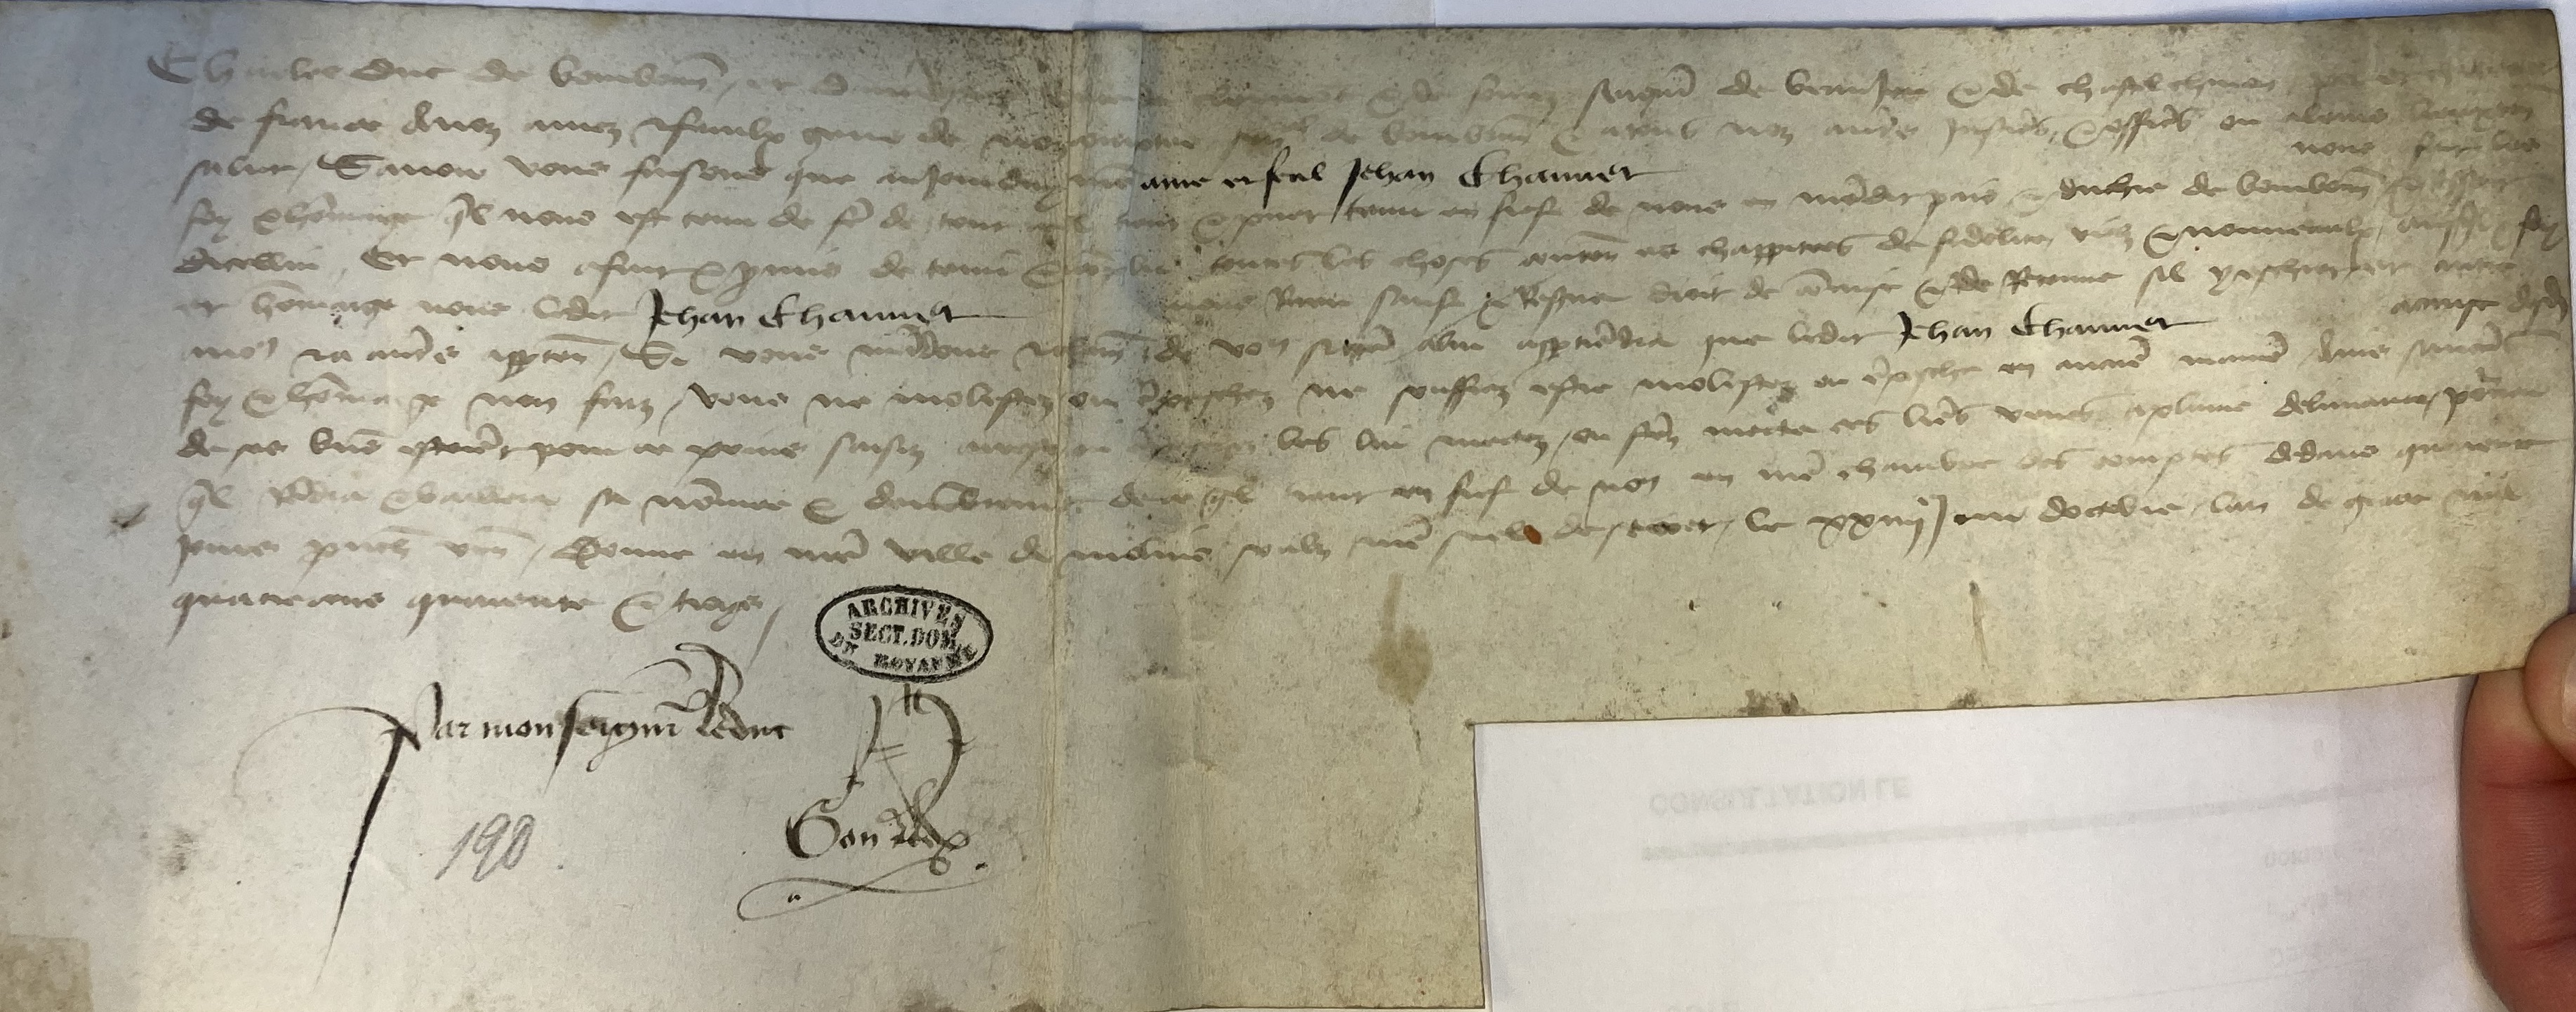
\includegraphics[scale =0.13]{img/IMG-2553.jpg}
\caption*{Acte daté du 24 octobre 1443.}
\label{IMG-2553}
\end{figure}

\begin{figure}[ht]
\centering
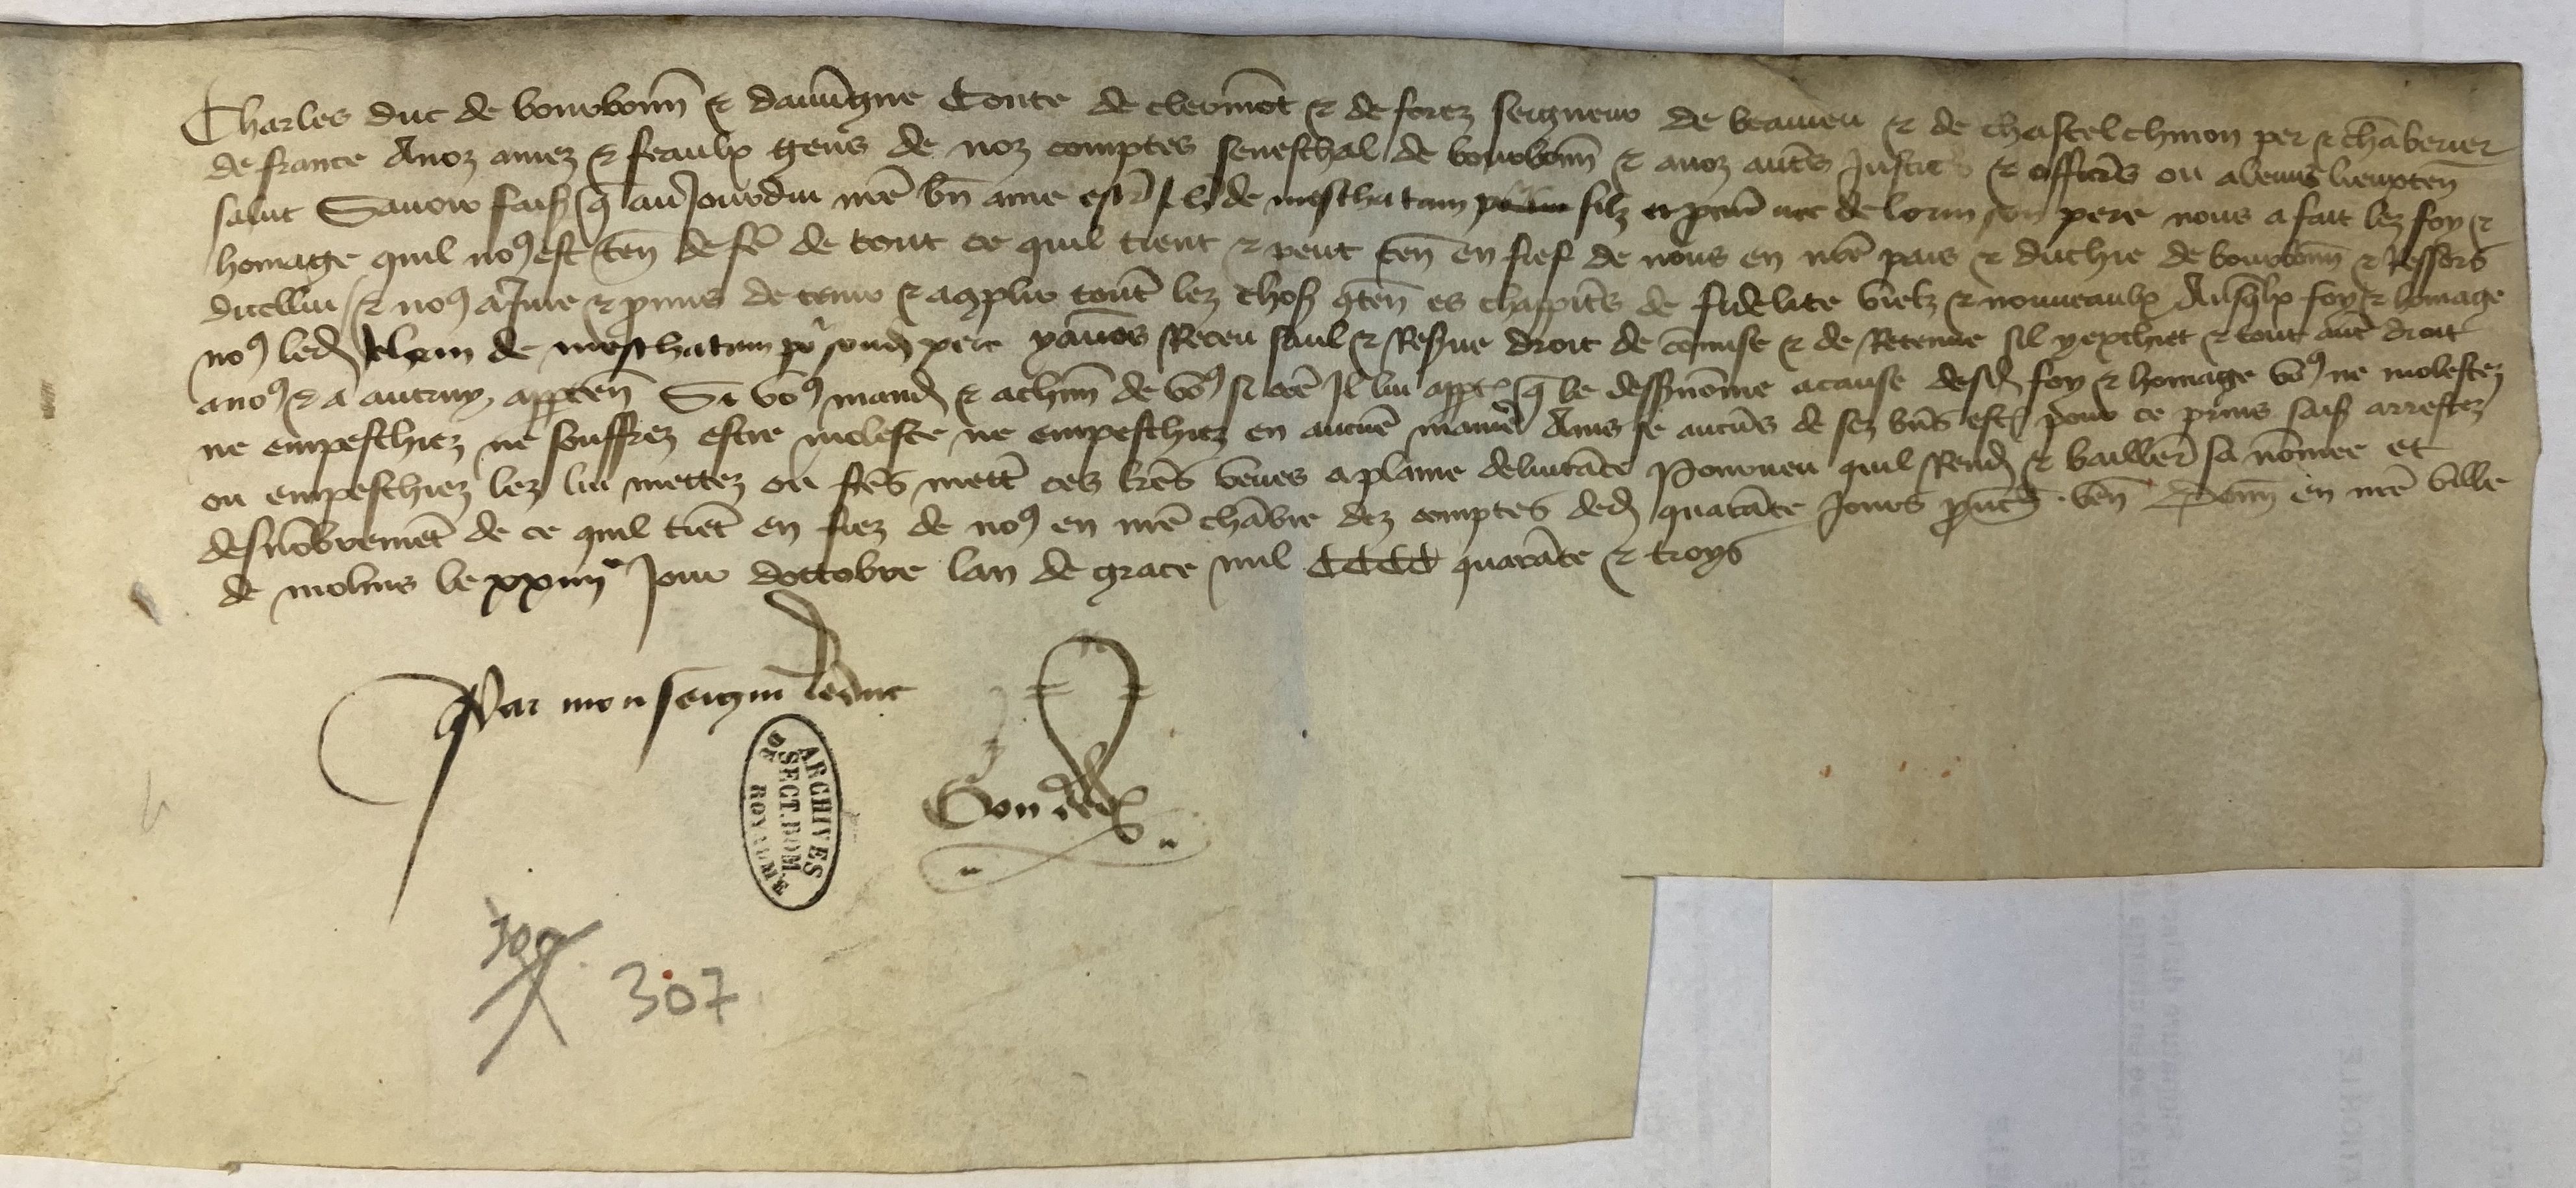
\includegraphics[scale =0.12]{img/IMG-2568.jpg}
\caption*{Acte daté du 24 octobre 1443.}
\label{IMG-2568}
\end{figure}

\begin{figure}[ht]
\centering
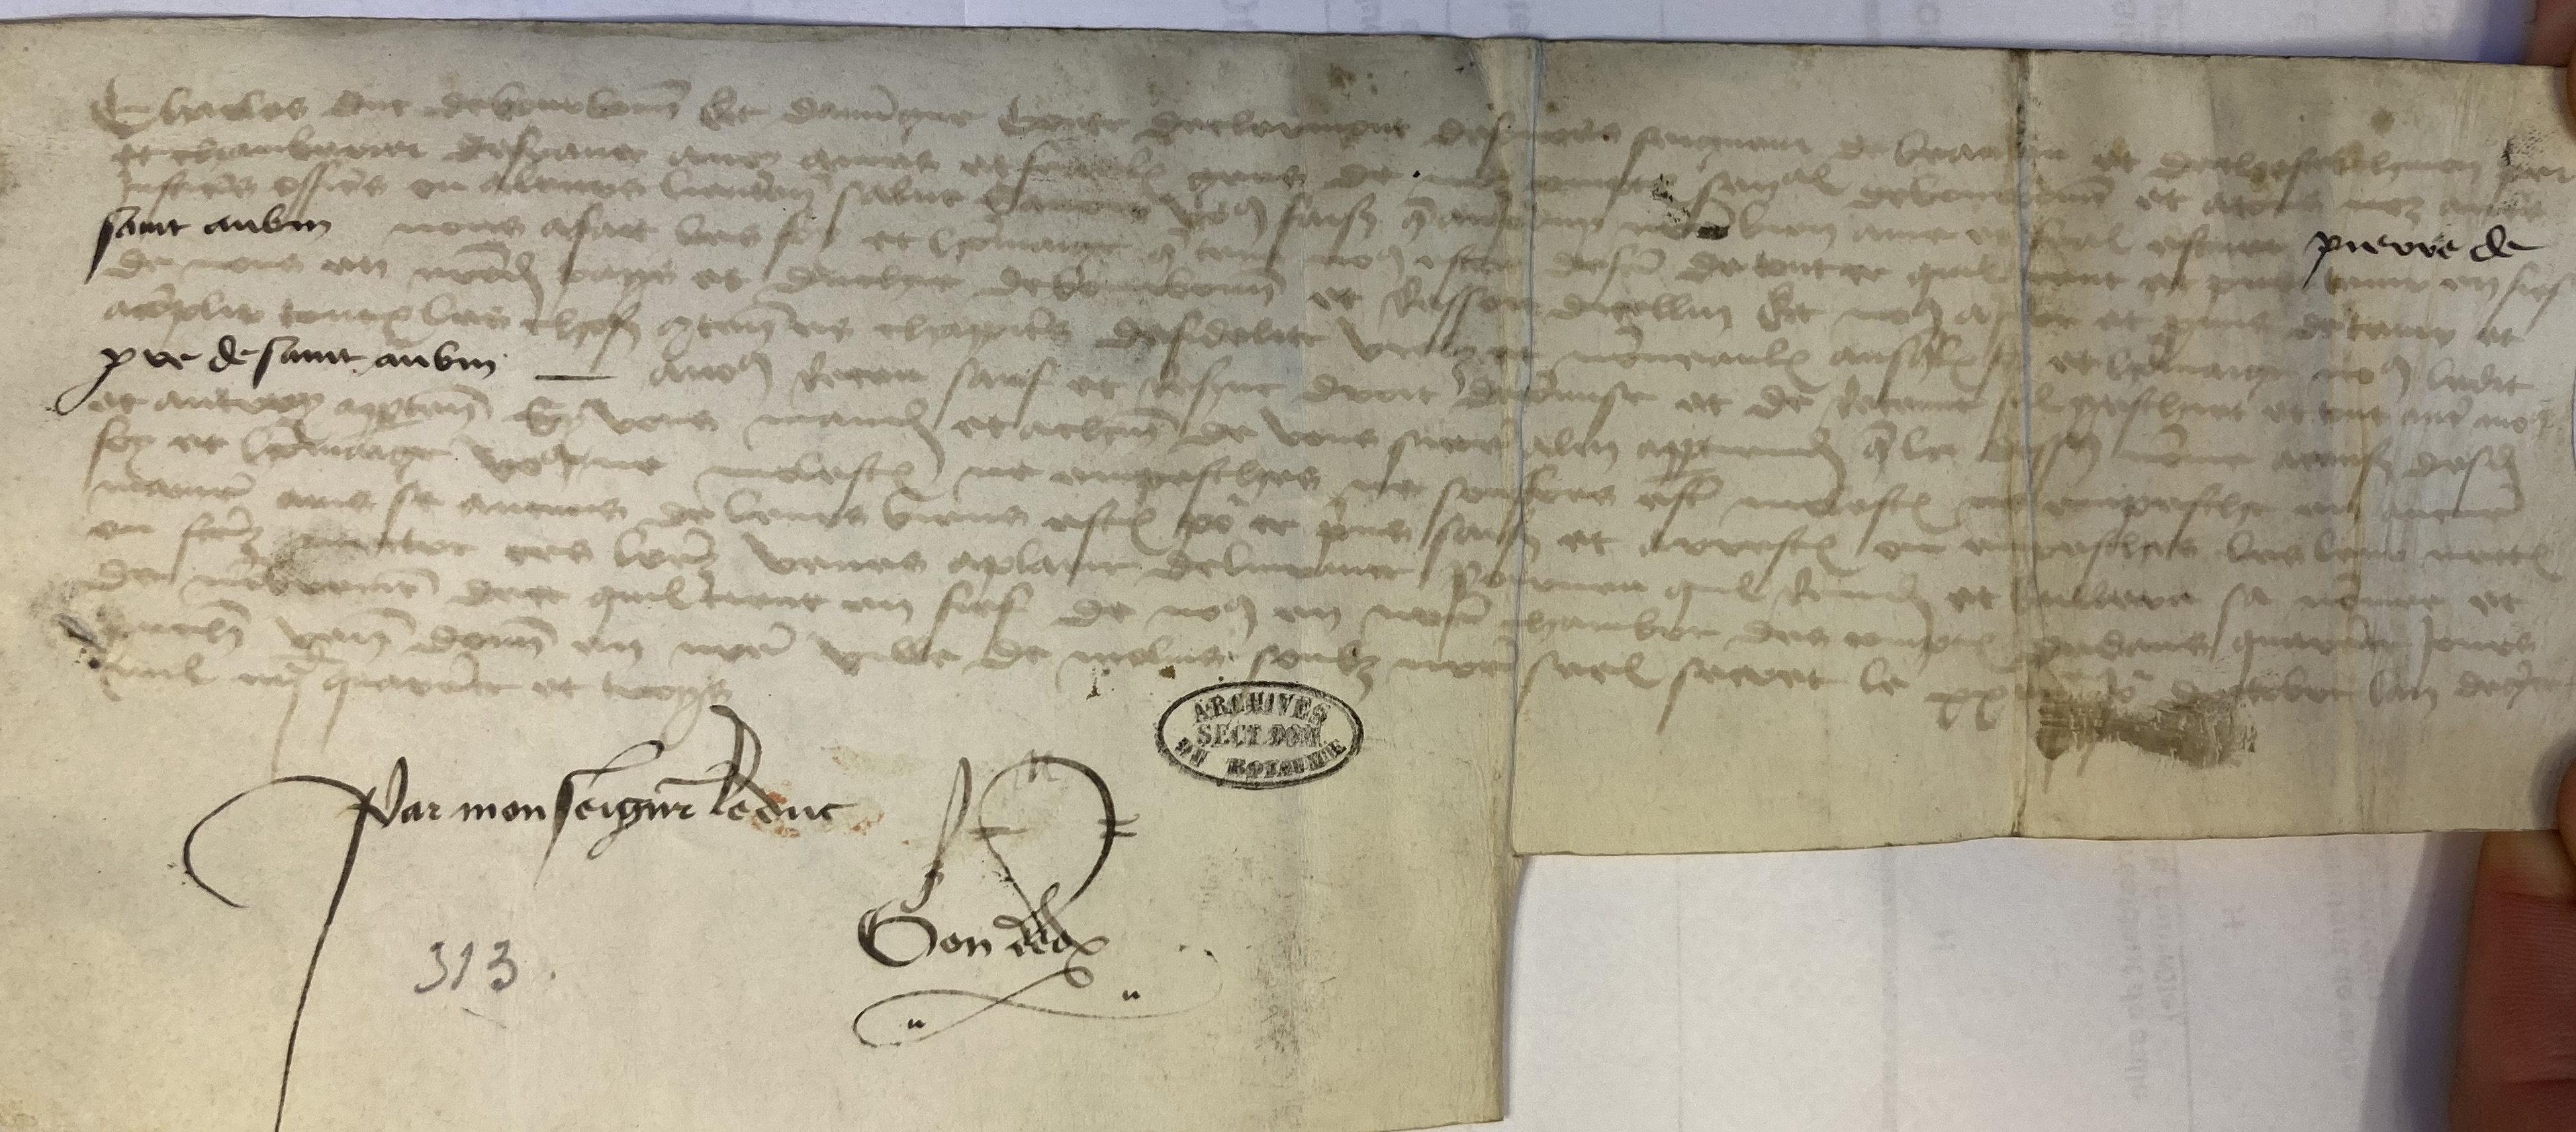
\includegraphics[scale =0.12]{img/IMG-2573.jpg}
\caption*{Acte daté du 24 octobre 1443.}
\label{IMG-2573}
\end{figure}

\begin{figure}[ht]
\centering
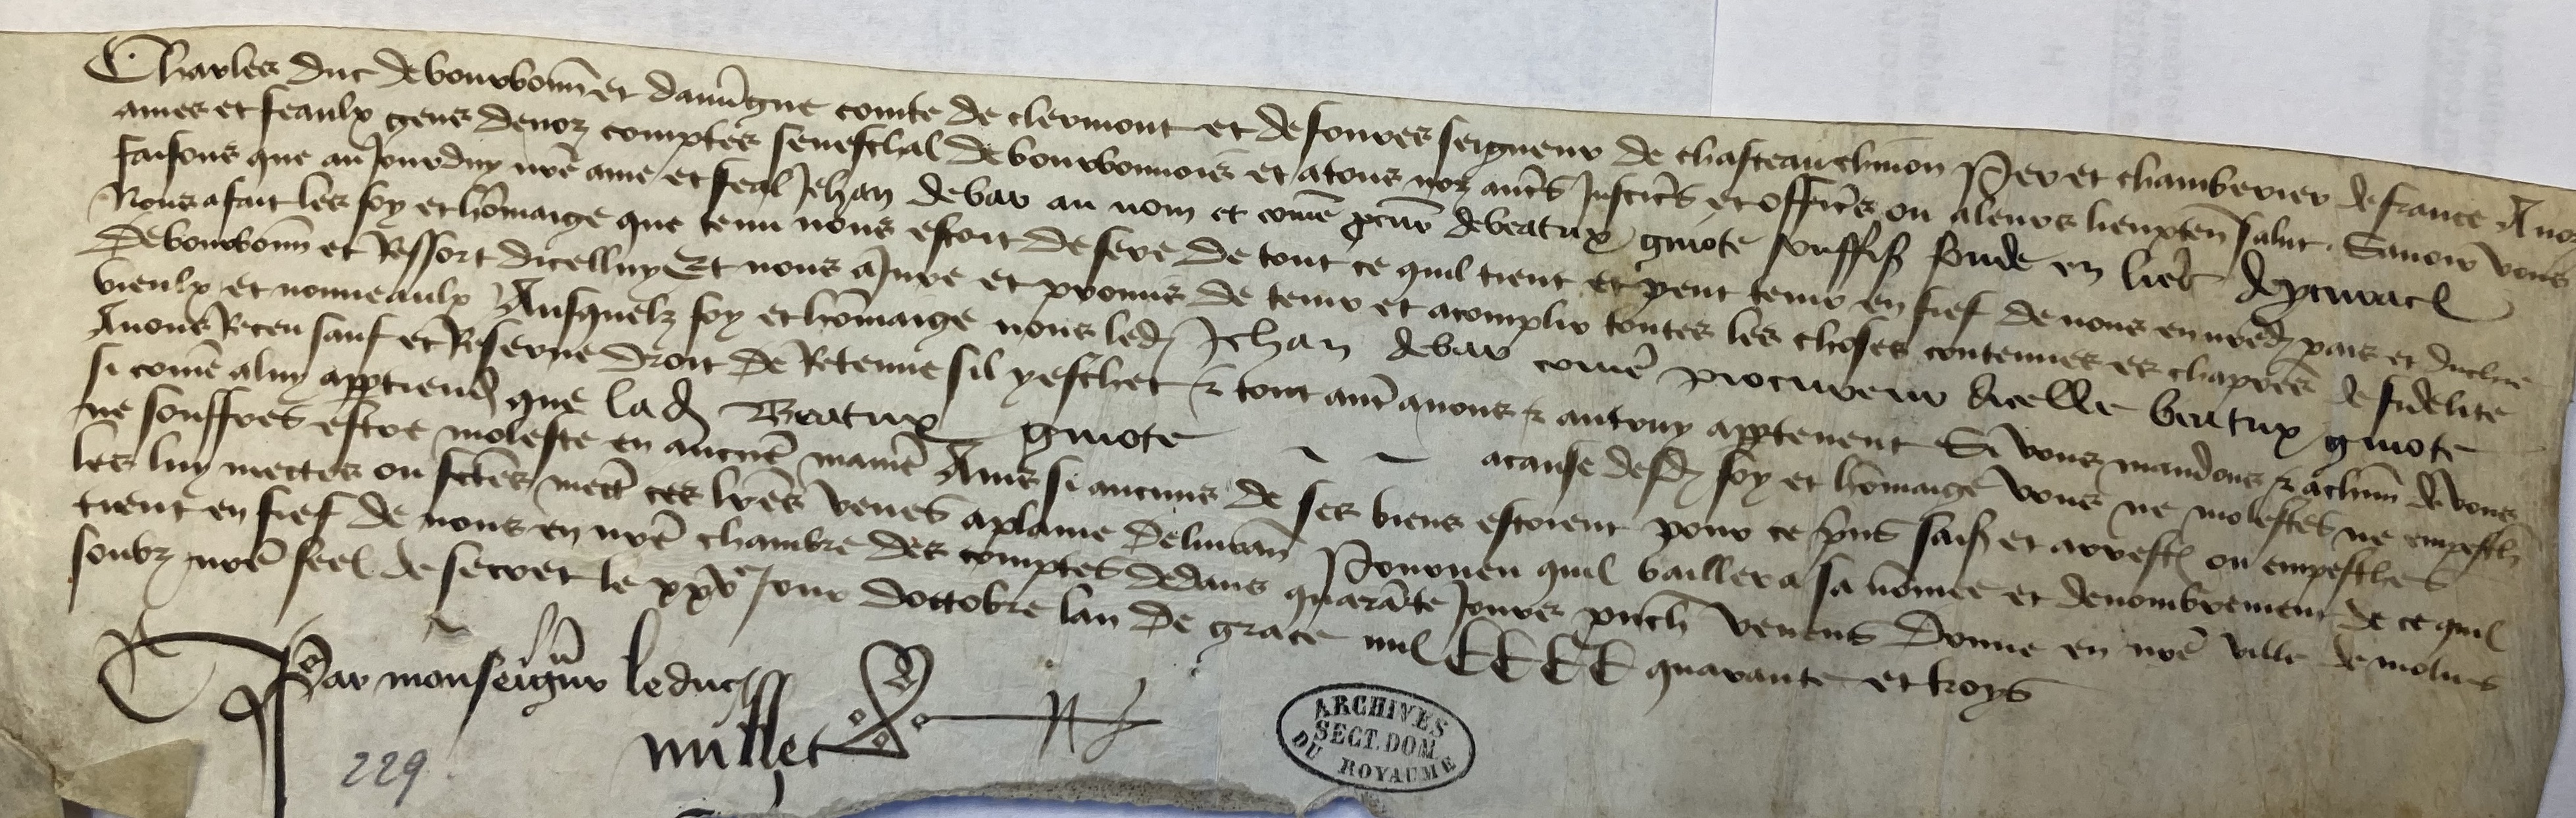
\includegraphics[scale =0.12]{img/IMG-2558.jpg}
\caption*{Acte daté du 25 octobre 1443.}
\label{IMG-2558}
\end{figure}

\begin{figure}[ht]
\centering
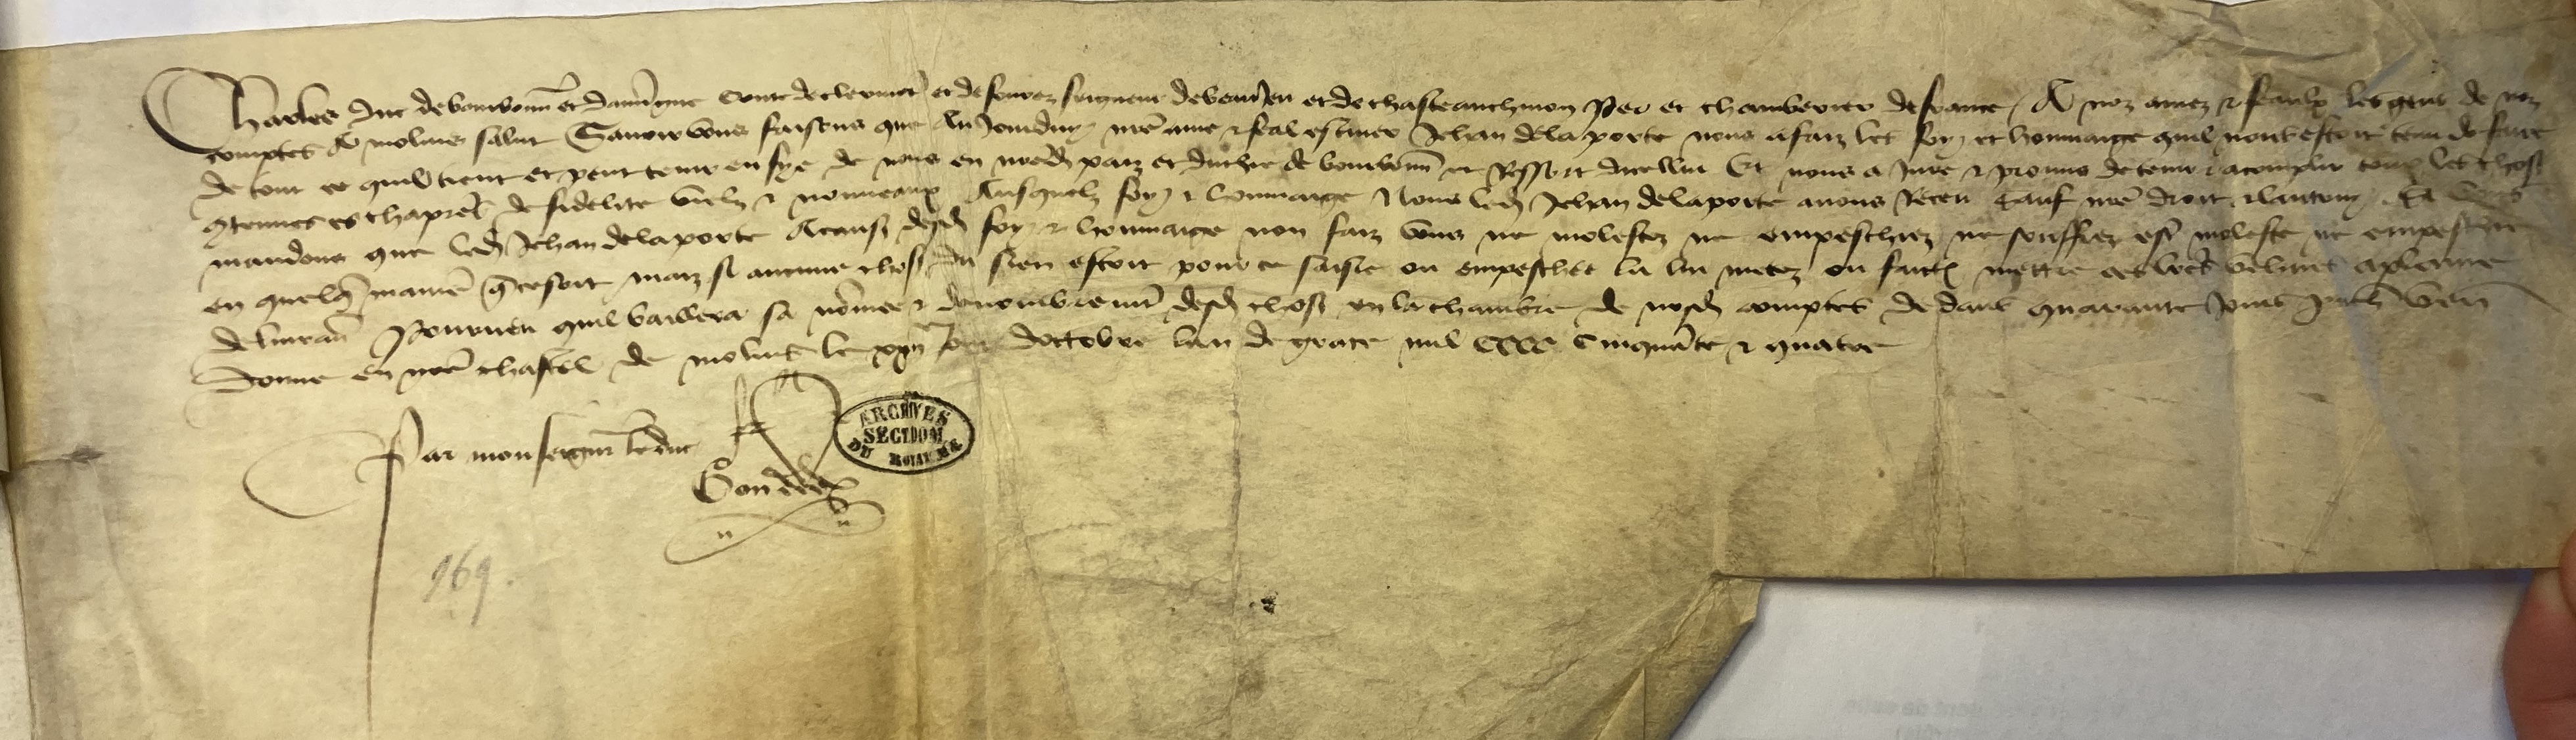
\includegraphics[scale =0.12]{img/IMG-2547.jpg}
\caption*{Acte daté du 22 octobre 1454.}
\label{IMG-2547}
\end{figure}
	
	

% index à mettre ici si index	
%	\printindex

% glossaire si glossaire
%	\printglossaries

% si figures
%	\listoffigures

% si tables
%	\listoftables

	\tableofcontents
	
\end{document}